\chapter{分类}
\label{chap:classification}

判断邮件是否为垃圾邮件，需要从预设类别中作出选择。\term{分类}（classification）从带标签样本学习这种决策。设$D_n=\{(\bm{x}_i,y_i)\}_{i=1}^{n}$，$\bm{x}_i\in\mathbb{R}^{d}$、$y_i\in\{1,\dots,C\}$，分类器为$f:\mathbb{R}^{d}\to\{1,\dots,C\}$；预测类别发生变化的位置构成\term{决策边界}（decision boundary）。本章讨论每个样本属于一个预设类别的单标签分类。

1930年代的Fisher判别分析从投影区分类别，1950年代的感知机通过错分反馈学习边界。决策树在1980年代形成系统方法，1990年代的支持向量机把间隔与核方法结合起来，此后的树集成进一步提高了复杂数据上的预测能力\scite{fisher1936,rosenblatt1958,cortes1995}

在高维稀疏文本等任务中，线性分类器与朴素贝叶斯仍便于建立基线；在异质表格数据上，随机森林与梯度提升树是常用候选，需要与其他方法在相同预算下比较\scite{erickson2026tabarena}本章按线性关系、邻域、树与规则、概率和集成展开：它们分别学习得分、聚合局部标签、使用条件分支、估计类别概率或组合成员；半监督分类随后说明怎样利用未标注样本。

除特别说明外，统计分析假设训练样本独立同分布，新样本独立来自同一分布。零一损失风险记为$R(f)=\mathbb{P}(f(\bm{x})\ne y)$，所有可测分类规则的最小风险记为$R^\ast$，即贝叶斯风险；其学习理论基础见
\BookChapterRef{chap:binary-learnability}{第二卷“基础、理论和可信性”的“二分类学习的可学习性”章}。

\section{基于线性关系的分类}
\label{sec:classification-geometry}

第\ref{sec:classic-overview-linear}节的线性得分在分类中用于比较类别。本节从LDA、感知机和SVM考察三种学习依据：类统计量、分类错误反馈和间隔。相同的线性边界可以来自不同准则；随后用简介已建立的核方法扩展SVM的特征空间。

LDA兼有投影与概率解释，本节推导其共享协方差形式，第\ref{sec:classification-probability}节再从GDA模型族说明一般协方差设定。Fisher投影的统计量、感知机的可分性条件与软间隔SVM的误差容忍约束不同对象，不能排成假设强度依次递减的序列。

\subsection{线性判别分析（LDA）}
\label{sec:classification-lda}

如果用一个线性得分区分类别，怎样确定各特征的权重和分类阈值？一种办法是先描述每一类样本在空间中的分布，再比较新样本来自各类的可能性。\term{线性判别分析}（linear discriminant analysis, LDA）在高斯生成模型下采用这条路线：估计类均值、共享协方差和类先验，再由贝叶斯法则得到线性判别函数。

LDA还有一个几何起点。Fisher在1936年的鸢尾花分类研究中寻找一种线性组合，使两类均值的差异相对于类内波动尽可能大。这一准则不要求样本服从高斯分布；它与高斯生成模型可以给出相同的判别方向，但概率解释和适用条件有所不同\scite{fisher1936}

从两类的线性组合转向多个总体的判别，问题不再只是选择一条轴，还包括需要保留多少个方向。Rao在1948年系统讨论了多总体的生物分类与判别表示，这也为理解LDA如何从分类规则延伸为有监督降维方法提供了历史背景\scite{rao1948}

\subsubsection{模型结构}
\label{sec:classification-lda-model}

沿用训练集$D_n=\{(\bm{x}_i,y_i)\}_{i=1}^{n}$，其中$\bm{x}_i\in\mathbb{R}^{d}$、$y_i\in\{1,\ldots,C\}$。生成式LDA假设
\begin{equation}
  \label{eq:classification-lda-distribution}
  \begin{aligned}
    \mathbb{P}(y=c)&=\pi_c,\qquad \pi_c>0,\quad
      \sum_{c=1}^{C}\pi_c=1,\\
    p(\bm{x}\mid y=c)&=\mathcal{N}(\bm{x};\bm{\mu}_c,\bm{\Sigma}),
      \qquad \bm{\Sigma}\succ0 .
  \end{aligned}
\end{equation}
这里$\bm{\mu}_c\in\mathbb{R}^{d}$描述第$c$类的中心，$\bm{\Sigma}\in\mathbb{R}^{d\times d}$描述类内各方向的波动及特征之间的相关性。共享协方差意味着各类可以有不同中心，但在中心附近具有相同的椭球形状和朝向；并不要求各个特征相互独立。

在零一损失下，应选择后验概率最大的类别。取对数并展开高斯密度，有
\begin{equation}
  \label{eq:classification-lda-score}
  \begin{aligned}
    \log\{\pi_c p(\bm{x}\mid y=c)\}
      &=a(\bm{x})+\delta_c(\bm{x}),\\
    \delta_c(\bm{x})
      &=\bm{x}^{\top}\bm{\Sigma}^{-1}\bm{\mu}_c\\
      &\quad-\frac12\bm{\mu}_c^{\top}\bm{\Sigma}^{-1}\bm{\mu}_c
        +\log\pi_c .
  \end{aligned}
\end{equation}
其中$a(\bm{x})$收集了$-\bm{x}^{\top}\bm{\Sigma}^{-1}\bm{x}/2$、对数行列式和高斯归一化常数，均与类别无关。正是共享协方差使二次项在类别比较时抵消，留下关于$\bm{x}$的仿射函数。任意两类得分相等的位置通常为超平面；多分类时，各类别区域由若干这样的比较共同确定，而不是全体类别只共用一个分割面。

训练后把估计参数代入$\delta_c$，得到$\hat{\delta}_c$。预测规则及相应的模型后验为
\begin{equation}
  \label{eq:classification-lda-prediction}
  \begin{aligned}
    \hat f_{\mathrm{LDA}}(\bm{x})
      &=\argmax_{c\in\{1,\ldots,C\}}\hat{\delta}_c(\bm{x}),\\
    \hat p_c(\bm{x})
      &=\frac{\exp\{\hat{\delta}_c(\bm{x})\}}
        {\sum_{j=1}^{C}\exp\{\hat{\delta}_j(\bm{x})\}} .
  \end{aligned}
\end{equation}
本节对$\argmax$的平局统一选择索引最小的类别。若放宽共享协方差约束，让每类使用自己的$\bm{\Sigma}_c$，二次项便不再普遍抵消，得到\term{二次判别分析}（quadratic discriminant analysis, QDA），即允许二次决策边界的高斯分类器\scite{hastie2009}

\subsubsection{参数学习}
\label{sec:classification-lda-learning}

\paragraph{生成模型的最大似然估计}
有标签样本已经给出了每个观测所属的高斯分量，因此这里不需要推断类别归属。令$n_c=\sum_{i=1}^{n}\mathbb{1}\{y_i=c\}$，暂设各类都有样本。忽略与参数无关的常数，对数似然为
\begin{equation}
  \label{eq:classification-lda-likelihood}
  \begin{aligned}
    \ell
      &=\sum_{c=1}^{C}n_c\log\pi_c
        -\frac n2\log\det\bm{\Sigma}\\
      &\quad-\frac12\sum_{c=1}^{C}\sum_{i:y_i=c}
        (\bm{x}_i-\bm{\mu}_c)^{\top}
        \bm{\Sigma}^{-1}(\bm{x}_i-\bm{\mu}_c).
  \end{aligned}
\end{equation}
对先验加入约束$\sum_c\pi_c=1$，拉格朗日驻点给出$n_c/\pi_c$为同一常数；归一化后该常数为$n$。对$\bm{\mu}_c$求导，则有$\bm{\Sigma}^{-1}\sum_{i:y_i=c}(\bm{x}_i-\bm{\mu}_c)=\bm{0}$。由此得到
\begin{equation}
  \label{eq:classification-lda-mean-prior}
  \hat\pi_c=\frac{n_c}{n},\qquad
  \hat{\bm{\mu}}_c=\frac1{n_c}\sum_{i:y_i=c}\bm{x}_i .
\end{equation}
这两个估计分别是类别出现频率和该类的样本均值。

把均值代回似然，定义\term{类内散度矩阵}（within-class scatter matrix）
\begin{equation}
  \label{eq:classification-lda-within}
  \bm{S}_{\mathrm{W}}
    =\sum_{c=1}^{C}\sum_{i:y_i=c}
      (\bm{x}_i-\hat{\bm{\mu}}_c)
      (\bm{x}_i-\hat{\bm{\mu}}_c)^{\top}.
\end{equation}
它累加每个样本相对于本类中心的偏离。用精度矩阵$\bm{\Omega}=\bm{\Sigma}^{-1}$改写剩余目标，得到$n\log\det\bm{\Omega}/2-\operatorname{tr}(\bm{\Omega}\bm{S}_{\mathrm{W}})/2$。其驻点满足$n\bm{\Omega}^{-1}=\bm{S}_{\mathrm{W}}$，故当$\bm{S}_{\mathrm{W}}\succ0$时，
\begin{equation}
  \label{eq:classification-lda-covariance}
  \hat{\bm{\Sigma}}=\frac1n\bm{S}_{\mathrm{W}} .
\end{equation}
对$\bm{\Omega}$的目标是严格凹的，因此该驻点给出最大似然解。

式~\eqref{eq:classification-lda-covariance}的分母是$n$，不是$n-C$。这种合并各类类内变动的估计称为\term{合并协方差}（pooled covariance），其无偏形式为
\[
  \hat{\bm{\Sigma}}_{\mathrm{U}}
    =\frac{\bm{S}_{\mathrm{W}}}{n-C},\qquad n>C .
\]
在共享协方差假设下，给定各类样本数，有$\mathbb{E}[\bm{S}_{\mathrm{W}}\mid y_1,\ldots,y_n]=(n-C)\bm{\Sigma}$，因为估计每个类中心各消耗一个自由度。最大似然与无偏估计是不同准则；两种估计渐近相同，但有限样本下有所区别。特别是先验不等时，整体缩放协方差会改变几何得分相对于$\log\hat\pi_c$的权重，预测边界未必相同。

闭式估计不等于没有计算代价。对稠密数据，累积类内散度需要$O(nd^2)$运算，矩阵分解需要$O(d^3)$运算。实现时分解一次$\hat{\bm{\Sigma}}$，再解$C$个线性方程组$\hat{\bm{\Sigma}}\bm{a}_c=\hat{\bm{\mu}}_c$，预存$\bm{a}_c$和常数得分项；不必显式求逆，预测一个样本只需$O(Cd)$运算。若$\bm{S}_{\mathrm{W}}$奇异，正定参数域内上述最大似然解并不存在，需要降低维数或作正则化，不能直接使用逆矩阵公式。

\paragraph{Fisher投影的学习}
生成模型之外，还可以直接比较投影后的类间分离与类内波动。令总样本均值$\hat{\bm{\mu}}=\sum_c(n_c/n)\hat{\bm{\mu}}_c$，定义\term{类间散度矩阵}（between-class scatter matrix）
\[
  \bm{S}_{\mathrm{B}}
    =\sum_{c=1}^{C}n_c
      (\hat{\bm{\mu}}_c-\hat{\bm{\mu}})
      (\hat{\bm{\mu}}_c-\hat{\bm{\mu}})^{\top}.
\]
它衡量各类中心相对于总中心的分散程度。投影到方向$\bm{w}$后，两种散度分别变为$\bm{w}^{\top}\bm{S}_{\mathrm{B}}\bm{w}$和$\bm{w}^{\top}\bm{S}_{\mathrm{W}}\bm{w}$。\term{Fisher判别准则}（Fisher discriminant criterion）取两者之比。以下假设$\bm{S}_{\mathrm{W}}\succ0$，使每个非零方向的分母都为正：
\begin{equation}
  \label{eq:classification-fisher-criterion}
  J(\bm{w})
    =\frac{\bm{w}^{\top}\bm{S}_{\mathrm{B}}\bm{w}}
      {\bm{w}^{\top}\bm{S}_{\mathrm{W}}\bm{w}},
    \qquad \bm{w}\ne\bm{0}.
\end{equation}
分子鼓励类中心远离，分母抑制同类样本投影后过于分散。

图~\ref{fig:classification-lda-projection}固定同一组二维教学样本，只改变投影方向。沿$\bm{w}_{\mathrm{A}}=(1,0)^{\top}$，两类投影均值相差$2$，而各类仅在宽度$0.6$的区间内波动；沿$\bm{w}_{\mathrm{B}}=(3/5,4/5)^{\top}$，均值差缩为$1.2$，同类投影却散布得更宽，异类点在数轴上交错。由图注中的构造可算得$\bm{S}_{\mathrm{W}}=\operatorname{diag}(2/5,8)$、$\bm{S}_{\mathrm{B}}=\operatorname{diag}(8,0)$，所以$J(\bm{w}_{\mathrm{A}})=20$，$J(\bm{w}_{\mathrm{B}})=180/329$。这个比较衡量的是同一批样本投影后的相对分离程度，不是测试错误率。

\begin{figure}[htbp]
  \centering
  % 两类中心为 (-1,0)、(1,0)，共用四个精确十进制偏移；不使用随机点或抖动。
% 两面板均由同一偏移表生成，投影坐标直接计算为 wx*x1+wy*x2。
\begin{tikzpicture}[
  x=0.1\linewidth,y=0.1\linewidth,
  font=\footnotesize,
  every node/.style={inner sep=1pt}
]
  \path[use as bounding box] (0,-4.3) rectangle (10,2.4);
  \foreach \shift/\id/\wx/\wy/\pattern/\comparison/\ratio in {
    2.3/A/1/0/solid/较大/20,
    7.6/B/0.6/0.8/dashed/较小/{180/329}
  } {
    \begin{scope}[shift={(\shift,0)}]
      \node[font=\heiti\footnotesize] at (0,2.1)
        {（\id）相对分离\comparison};
      \draw[BookMuted,thin,-{Stealth[length=1.3mm]}]
        (-1.75,0) -- (1.85,0) node[right] {$x_1$};
      \draw[BookMuted,thin,-{Stealth[length=1.3mm]}]
        (0,-1.25) -- (0,1.4) node[above] {$x_2$};
      \foreach \tick in {-1,1} {
        \draw[BookMuted] (\tick,-0.04) -- (\tick,0.04);
        \node[below] at (\tick,-0.06) {$\tick$};
        \draw[BookMuted] (-0.04,\tick) -- (0.04,\tick);
        \node[left] at (-0.06,\tick) {$\tick$};
      }
      \node[below left] at (0,0) {$0$};
      \draw[BookTeal,thick,\pattern,-{Stealth[length=1.5mm]}]
        (0,0) -- ({1.45*\wx},{1.45*\wy})
        node[above right] {$\bm{w}_{\mathrm{\id}}$};

      \node at (0,-1.65) {$z_{\mathrm{\id}}=\bm{w}_{\mathrm{\id}}^{\top}\bm{x}$};
      \foreach \class/\cx/\colour/\row in {
        1/-1/BookBlue/-2.1,
        2/1/BookAmber/-2.5
      } {
        \draw[BookRule] (-1.75,\row) -- (1.75,\row);
        \foreach \dx/\dy in {-0.3/-1,-0.1/1,0.1/1,0.3/-1} {
          \pgfmathsetmacro{\px}{\cx+\dx}
          \pgfmathsetmacro{\pz}{\wx*\px+\wy*\dy}
          \ifnum\class=1
            \fill[\colour] (\px,\dy) circle (1.5pt);
            \fill[\colour] (\pz,\row) circle (1.5pt);
          \else
            \fill[\colour] ([xshift=-1.5pt,yshift=-1.5pt]\px,\dy)
              rectangle ++(3pt,3pt);
            \fill[\colour] ([xshift=-1.5pt,yshift=-1.5pt]\pz,\row)
              rectangle ++(3pt,3pt);
          \fi
        }
        \pgfmathsetmacro{\mz}{\wx*\cx}
        \draw[\colour,line width=0.8pt]
          (\mz,{\row-0.13}) -- (\mz,{\row+0.13});
      }
      \draw[BookMuted,thin,-{Stealth[length=1.3mm]}]
        (-1.75,-2.9) -- (1.85,-2.9) node[right] {$z$};
      \foreach \tick in {-1,0,1} {
        \draw[BookMuted] (\tick,-2.94) -- (\tick,-2.86);
        \node[below] at (\tick,-2.97) {$\tick$};
      }
      \node at (0,-3.5) {$J(\bm{w}_{\mathrm{\id}})=\ratio$};
    \end{scope}
  }
  \fill[BookBlue] (1.8,-4.05) circle (1.5pt);
  \node[right] at (2,-4.05) {类1};
  \fill[BookAmber] ([xshift=-1.5pt,yshift=-1.5pt]4,-4.05)
    rectangle ++(3pt,3pt);
  \node[right] at (4.2,-4.05) {类2};
  \draw[BookInk,line width=0.8pt] (6.1,-4.18) -- (6.1,-3.92);
  \node[right] at (6.3,-4.05) {投影均值};
\end{tikzpicture}

  \caption{同一点集在两个单位方向上的投影。两类各有4点，中心分别为$(-1,0)^{\top}$、$(1,0)^{\top}$，都加上偏移$(-0.3,-1)^{\top}$、$(-0.1,1)^{\top}$、$(0.1,1)^{\top}$、$(0.3,-1)^{\top}$；这是人为构造，坐标无量纲。两行只改变黄色投影方向：$\bm{w}_{\mathrm{A}}=(1,0)^{\top}$与$\bm{w}_{\mathrm{B}}=(3/5,4/5)^{\top}$。右侧按$z=\bm{w}^{\top}\bm{x}$把蓝圆和红方放到同一数轴，彩色短竖线标出各类投影均值；两行共用数轴尺度。}
  \label{fig:classification-lda-projection}
\end{figure}

由于$J$不受$\bm{w}$的非零倍数缩放影响，可以约束$\bm{w}^{\top}\bm{S}_{\mathrm{W}}\bm{w}=1$。对$\bm{w}^{\top}\bm{S}_{\mathrm{B}}\bm{w}-\lambda(\bm{w}^{\top}\bm{S}_{\mathrm{W}}\bm{w}-1)$求导，得到\term{广义特征值问题}（generalized eigenvalue problem）：
\begin{equation}
  \label{eq:classification-fisher-eigenproblem}
  \bm{S}_{\mathrm{B}}\bm{w}
    =\lambda\bm{S}_{\mathrm{W}}\bm{w}.
\end{equation}
驻点还需比较大小。令$\bm{v}=\bm{S}_{\mathrm{W}}^{1/2}\bm{w}$，则
\[
  J(\bm{w})=\frac{\bm{v}^{\top}\bm{A}\bm{v}}{\bm{v}^{\top}\bm{v}},
  \qquad
  \bm{A}=\bm{S}_{\mathrm{W}}^{-1/2}
    \bm{S}_{\mathrm{B}}\bm{S}_{\mathrm{W}}^{-1/2}.
\]
把$\bm{v}$展开到对称半正定矩阵$\bm{A}$的正交特征向量上，上式就是各特征值的加权平均，权重非负且总和为$1$。最大值因而是最大特征值；取对应特征向量，再乘$\bm{S}_{\mathrm{W}}^{-1/2}$，便得到最优Fisher方向。若最大特征值有重数，最优方向未必唯一。

二分类时，令$\bm{h}=\hat{\bm{\mu}}_1-\hat{\bm{\mu}}_2\ne\bm{0}$，由总均值的定义可得
\[
  \bm{S}_{\mathrm{B}}=\frac{n_1n_2}{n}\bm{h}\bm{h}^{\top},
  \qquad
  \bm{w}_{\mathrm{F}}\propto\bm{S}_{\mathrm{W}}^{-1}\bm{h}.
\]
生成式LDA的法向量则为$\bm{w}_{\mathrm{G}}=\hat{\bm{\Sigma}}^{-1}\bm{h}=n\bm{S}_{\mathrm{W}}^{-1}\bm{h}$，两者方向相同。但完整的生成式分类规则还比较
\begin{equation}
  \label{eq:classification-lda-binary-threshold}
  \hat\delta_1(\bm{x})-\hat\delta_2(\bm{x})
    =\bm{w}_{\mathrm{G}}^{\top}
      \left(\bm{x}-\frac{\hat{\bm{\mu}}_1+\hat{\bm{\mu}}_2}{2}\right)
      +\log\frac{\hat\pi_1}{\hat\pi_2}
\end{equation}
的正负。Fisher准则本身只给方向，不给类先验、后验概率或这一阈值。两类均值相同时，均值散度准则没有正特征值方向，而生成模型仍可按先验选择类别。由此可见，非高斯数据上仍能使用Fisher投影，但不能据此沿用高斯LDA的贝叶斯最优性结论。

\subsubsection{理论分析}
\label{sec:classification-lda-analysis}

\paragraph{收敛性分析}
生成式LDA的均值、先验与协方差都有闭式估计，因此这里考察的是样本量增加时估计是否趋近真实参数，而不是某个迭代过程何时停止。\term{一致性}（consistency）正是这种渐近性质；它不表示某个有限训练集上的估计已经准确。

\begin{theorem}[LDA参数估计的一致性]
  \label{thm:classification-lda-consistency}
  设$d$和$C$固定，训练样本独立同分布，真实分布满足式~\eqref{eq:classification-lda-distribution}，且所有$\pi_c^\ast>0$、$\bm{\Sigma}^\ast\succ0$。当$n\to\infty$时，
  \[
    \hat\pi_c\xrightarrow{\mathbb{P}}\pi_c^\ast,\qquad
    \hat{\bm{\mu}}_c\xrightarrow{\mathbb{P}}\bm{\mu}_c^\ast,\qquad
    \hat{\bm{\Sigma}}\xrightarrow{\mathbb{P}}\bm{\Sigma}^\ast .
  \]
  所有类别非空且$\hat{\bm{\Sigma}}$正定的概率趋于$1$。
\end{theorem}

\begin{proof}
  为处理随机的$n_c$，把类均值写成两个全样本平均之比：
  \[
    \hat{\bm{\mu}}_c
      =\frac{n^{-1}\sum_{i=1}^{n}\bm{x}_i\mathbb{1}\{y_i=c\}}
        {n^{-1}\sum_{i=1}^{n}\mathbb{1}\{y_i=c\}} .
  \]
  大数定律使分母收敛到$\pi_c^\ast>0$，分子收敛到$\pi_c^\ast\bm{\mu}_c^\ast$，因而先验和均值都一致。尚未观察到某一类时可以任意约定其均值；该事件的概率趋于零，不影响结论。

  共享协方差估计可展开为
  \[
    \hat{\bm{\Sigma}}
      =\frac1n\sum_{i=1}^{n}\bm{x}_i\bm{x}_i^{\top}
        -\sum_{c=1}^{C}\hat\pi_c
          \hat{\bm{\mu}}_c\hat{\bm{\mu}}_c^{\top}.
  \]
  高斯分布有有限二阶矩，故第一项收敛到
  \[
    \mathbb{E}[\bm{x}\bm{x}^{\top}]
      =\bm{\Sigma}^\ast+
        \sum_{c=1}^{C}\pi_c^\ast
          \bm{\mu}_c^\ast(\bm{\mu}_c^\ast)^{\top}.
  \]
  第二项消去类中心对二阶矩的贡献，余下$\bm{\Sigma}^\ast$。固定维数下，矩阵逐元素收敛也给出算子范数收敛；由$\bm{\Sigma}^\ast$的最小特征值严格为正，估计矩阵以趋于$1$的概率可逆。上述步骤实际上可由强大数定律加强为几乎必然收敛。
\end{proof}

矩阵求逆和$\log\pi_c$在这些条件下连续，所以在参数几乎必然收敛的事件上，对每个固定输入$\bm{x}$，有$\hat\delta_c(\bm{x})\to\delta_c^\ast(\bm{x})$。但$\argmax$在平局处不连续：在真实最大得分唯一的输入处，估计类别最终等于该输入的唯一贝叶斯类别；平局处则未必如此。若最优类别平局的输入集合概率为零，就能进一步推出随机输入上的预测标签收敛。不同贝叶斯分类器在平局处可以选择不同标签，却有相同风险。

\paragraph{泛化分析}
参数趋近真实值以后，还需要说明这如何影响独立测试样本上的错误率。分类风险的一致性不必要求标签处处收敛。记$p_c^\ast(\bm{x})$为真实后验，$f^\ast$任选一个贝叶斯规则。由于$\hat f_{\mathrm{LDA}}$最大化$\hat p_c$，逐点有
\begin{equation}
  \label{eq:classification-lda-excess-risk}
  \begin{aligned}
    0&\leq p_{f^\ast(\bm{x})}^\ast(\bm{x})
      -p_{\hat f_{\mathrm{LDA}}(\bm{x})}^\ast(\bm{x})\\
      &\leq 2\max_{1\leq c\leq C}
          |\hat p_c(\bm{x})-p_c^\ast(\bm{x})| .
  \end{aligned}
\end{equation}
这个上界来自在两项之间分别加减相应的估计后验，并利用$\hat p_{\hat f_{\mathrm{LDA}}}\geq\hat p_{f^\ast}$。在参数几乎必然收敛的事件上，后验估计也对每个输入收敛；右端趋于零且不超过$2$。对与训练集独立、来自同一分布的测试输入积分，再用支配收敛定理，得到
\[
  R(\hat f_{\mathrm{LDA}}\mid D_n)
    \longrightarrow R^\ast
    \quad\text{几乎必然},
\]
其中$R(\hat f_{\mathrm{LDA}}\mid D_n)$是给定训练集后的测试错误率，$R^\ast$是贝叶斯错误率。有限样本中无法拟合时可暂用任意固定分类器，不改变这一渐近结论。这是模型正确指定、固定维数下的保证，不是对任意分布或$d$随$n$快速增长的普遍保证，也未给出有限样本的收敛速率。Fisher准则在当前训练集上取得最大值，不能替代这一风险分析。

\subsubsection{支持有监督降维}
\label{sec:classification-lda-reduction}

如果类别多于两个，一条投影轴可能不足以保留类中心之间的差异。把多个广义特征向量作为$\bm{W}\in\mathbb{R}^{d\times r}$的列，就可以把输入转换为$\bm{z}=\bm{W}^{\top}(\bm{x}-\hat{\bm{\mu}})\in\mathbb{R}^{r}$。以下仍假设$\bm{S}_{\mathrm{W}}\succ0$，并取$1\leq r\leq d$。

为避免重复选择同一方向，可要求不同投影轴在类内散度度量下正交：
\begin{equation}
  \label{eq:classification-lda-subspace}
  \max_{\bm{W}}\operatorname{tr}
       (\bm{W}^{\top}\bm{S}_{\mathrm{B}}\bm{W})
  \quad\text{满足}\quad
  \bm{W}^{\top}\bm{S}_{\mathrm{W}}\bm{W}=\bm{I}_r .
\end{equation}
在前述白化坐标中，该问题选择$\bm{A}$最大的$r$个特征值对应的正交方向，因而也就是式~\eqref{eq:classification-fisher-eigenproblem}中最大的$r$个广义特征值方向。

为什么有用的方向至多为$C-1$个？令$\bm{M}\in\mathbb{R}^{d\times C}$的第$c$列为$\sqrt{n_c}(\hat{\bm{\mu}}_c-\hat{\bm{\mu}})$，则
\[
  \bm{S}_{\mathrm{B}}=\bm{M}\bm{M}^{\top},\qquad
  \bm{M}
  \begin{pmatrix}\sqrt{n_1}\\ \vdots\\ \sqrt{n_C}\end{pmatrix}
  =\bm{0}.
\]
右侧列向量非零，说明$\bm{M}$的$C$列线性相关。因此$\operatorname{rank}(\bm{S}_{\mathrm{B}})\leq\min(d,C-1)$；可逆白化不改变秩，$\bm{A}$也至多有这么多个正特征值。若类中心还有额外的线性依赖，实际维数更低。这个限制针对类均值散度，不表示任意分类任务的全部信息都能无损压缩到$C-1$维；例如均值相同而协方差不同的类别，可能被该准则忽略。

LDA投影使用了标签，因此训练和验证时必须把它作为学习流程的一部分，在每个训练划分内重新估计投影，不能先用全体样本标签降维再评估。得到的低维特征可以交给近邻分类器等后续模型。第\ref{chap:dimensionality-reduction}章按保留信息的目标比较降维方法；其中第\ref{sec:dim-pca}节的PCA保留输入方差而不使用类别标签，LDA则保留类别均值相对于类内波动的判别信息。Fisherfaces人脸识别方法就是借助Fisher准则构造低维判别表示的一个具体例子\scite{belhumeur1997}

\subsubsection{小结}
\label{sec:classification-lda-summary}

LDA给线性得分提供了两种解释：共享协方差高斯模型给出概率、方向和阈值，Fisher准则则直接选择类中心相对分离的投影。两者在二分类且采用同一类内散度时给出相同方向，但概率解释和风险保证仍依赖额外假设。作为特征变换，LDA也用于语音识别；例如Haeb-Umbach与Ney研究了按语音类别学习线性变换，再与后续识别模型结合的方案\scite{haebumbach1992}

选用LDA时，需要同时考察分布近似和协方差的可估计性。偏离高斯不必然使分类失效，却使前述最优性证明不再适用；异常样本也会影响均值与协方差。由于$\operatorname{rank}(\bm{S}_{\mathrm{W}})\leq\min(d,n-C)$，当$n-C<d$时估计必然奇异，即使样本稍多于这个界也可能不稳定。降维或收缩协方差可以改善可计算性，但引入了新的选择及偏差，需要用独立验证评估。

\subsection{感知机}
\label{sec:classification-perceptron}

如果不估计类条件分布，能否直接根据分类结果调整边界？\term{感知机}（perceptron）的做法是用线性得分预测类别，遇到错误就修正权重。它不要求高斯分布；线性可分性是其有限次更新保证的条件，而不是运行算法的前提。Rosenblatt在1958年的论文中研究了感知机的学习机制，本节介绍的是其中广泛使用的线性阈值模型与误差修正规则\scite{rosenblatt1958}

这条研究路线也有硬件实现。康奈尔航空实验室建造的Mark I Perceptron将感知机思想实现为电子装置，但历史上的系统还包含感觉、关联和响应等组织，不能把它的全部结构等同于今天的单个线性分类器\scite{smithsonianMarkI}

\subsubsection{模型结构}
\label{sec:classification-perceptron-model}

本小节先使用二分类标签$y_i\in\{-1,+1\}$。为了使偏置在更新规则和收敛证明中始终处于同一坐标系，引入\term{增广向量}（augmented vector），即在输入末尾补一个恒为$1$的分量，并把偏置并入参数：
\begin{equation}
  \label{eq:classification-perceptron-augmented}
  \tilde{\bm{x}}=
    \begin{pmatrix}\bm{x}\\1\end{pmatrix},\qquad
  \tilde{\bm{w}}=
    \begin{pmatrix}\bm{w}\\b\end{pmatrix}
    \in\mathbb{R}^{d+1}.
\end{equation}
其中$\bm{w}\in\mathbb{R}^{d}$，$b\in\mathbb{R}$。分类规则为
\begin{equation}
  \label{eq:classification-perceptron-prediction}
  f(\bm{x})=\operatorname{sign}
    (\tilde{\bm{w}}^{\top}\tilde{\bm{x}})
    =\operatorname{sign}(\bm{w}^{\top}\bm{x}+b).
\end{equation}
约定$\operatorname{sign}(s)=+1$当$s\geq0$，否则为$-1$。非退化边界$\bm{w}^{\top}\bm{x}+b=0$是在$d$维输入空间中的$(d-1)$维超平面。它与二分类LDA具有相同的边界形式，但其参数不由类分布及先验推出，也不自动给出类别概率。

在这一表示下，正间隔可分是指存在单位向量$\bm{u}^\ast\in\mathbb{R}^{d+1}$和$\gamma>0$，使
\begin{equation}
  \label{eq:classification-perceptron-margin}
  \begin{aligned}
    y_i\langle\bm{u}^\ast,\tilde{\bm{x}}_i\rangle
      &\geq\gamma,\qquad i=1,\ldots,n,\\
    \|\bm{u}^\ast\|_2&=1,\qquad
    \|\tilde{\bm{x}}_i\|_2\leq R .
  \end{aligned}
\end{equation}
这里$R$约束的是增广输入，因此$R\geq\max_i\sqrt{\|\bm{x}_i\|_2^2+1}$。$\gamma$也是增广空间中的间隔；若$\bm{u}^\ast=(\bm{v}^{\top},a)^{\top}/\sqrt{\|\bm{v}\|_2^2+a^2}$，其分母包含偏置$a$，不同于原输入空间中以$\|\bm{v}\|_2$归一化的几何距离。有限训练集只要能被仿射超平面严格分开，就存在这样的正$\gamma$。

线性表示的边界也很具体。例如异或任务把$(0,0)$、$(1,1)$标为负类，把$(1,0)$、$(0,1)$标为正类。按上述平局规则，前两点要求$b<0$和$w_1+w_2+b<0$，后两点要求$w_1+b\geq0$和$w_2+b\geq0$。前两式相加与后两式相加，对同一个$w_1+w_2+2b$给出矛盾要求。Minsky与Papert在1969年的《Perceptrons》中系统研究了此类表示能力限制；改变输入特征或加入非线性隐藏层可以越过单个线性边界的限制，但那已经改变了模型族\scite{minsky1969}

\subsubsection{参数学习}
\label{sec:classification-perceptron-learning}

从$\tilde{\bm{w}}^{(0)}=\bm{0}$出发，若当前样本满足$y_i\langle\tilde{\bm{w}}^{(t)},\tilde{\bm{x}}_i\rangle\leq0$，便进行一次更新：
\begin{equation}
  \label{eq:classification-perceptron-update}
  \tilde{\bm{w}}^{(t+1)}
    =\tilde{\bm{w}}^{(t)}+\eta y_i\tilde{\bm{x}}_i,
    \qquad \eta>0 .
\end{equation}
这里$t$只数实际更新，学习率$\eta$保持不变。拆开最后一个分量，就是$\bm{w}\leftarrow\bm{w}+\eta y_i\bm{x}_i$和$b\leftarrow b+\eta y_i$。同一个样本的有符号得分增加$\eta\|\tilde{\bm{x}}_i\|_2^2$，所以更新确实朝修正当前判断的方向移动；但它可能同时破坏其他样本的正确分类，因而需要反复遍历。零得分也触发更新，即使按平局规则恰好预测为正确的正类，仍要求它离开边界。

\begin{algorithm}[带遍历上限的感知机训练]
  \label{alg:classification-perceptron}
  \begin{algorithmic}[1]
    \Require $D_n$，固定学习率$\eta>0$，最大遍历轮数$E\geq1$
    \Ensure 参数$\tilde{\bm{w}}$与是否已验证收敛的状态
    \State $\tilde{\bm{w}}\gets\bm{0}$
    \For{$e=1,\ldots,E$}
      \State $m\gets0$
      \For{$i=1,\ldots,n$}
        \State $\tilde{\bm{x}}_i\gets(\bm{x}_i^{\top},1)^{\top}$
        \If{$y_i\langle\tilde{\bm{w}},\tilde{\bm{x}}_i\rangle\leq0$}
          \State $\tilde{\bm{w}}\gets\tilde{\bm{w}}+\eta y_i\tilde{\bm{x}}_i$
          \State $m\gets m+1$
        \EndIf
      \EndFor
      \If{$m=0$}
        \State \Return $(\tilde{\bm{w}},\text{已收敛})$
      \EndIf
    \EndFor
    \State \Return $(\tilde{\bm{w}},\text{达到轮数上限})$
  \end{algorithmic}
\end{algorithm}

一整轮没有更新时，所有样本都是在同一个参数下得到严格正的有符号得分，才构成收敛证据。达到轮数上限只表示预算用尽，不能据此断言数据不可分。稠密实现每轮需要$O(nd)$运算，除训练集外只需$O(d)$参数空间；样本访问顺序可以改变输出的分隔面。

从优化角度看，定义\term{感知机损失}（perceptron loss）
\begin{equation}
  \label{eq:classification-perceptron-loss}
  \ell_{\mathrm{P}}(\tilde{\bm{w}};\bm{x}_i,y_i)
    =\max\{0,-y_i\langle\tilde{\bm{w}},\tilde{\bm{x}}_i\rangle\}.
\end{equation}
负得分处的梯度为$-y_i\tilde{\bm{x}}_i$，正得分处为$\bm{0}$；零得分处选择次梯度$-y_i\tilde{\bm{x}}_i$，就得到式~\eqref{eq:classification-perceptron-update}。这是逐样本次梯度更新；随机抽取样本时才相应成为随机次梯度下降。这里使用的是零间隔损失，不是标准的\term{合页损失}（hinge loss）$\max\{0,1-y_i\langle\tilde{\bm{w}},\tilde{\bm{x}}_i\rangle\}$。前者在零参数处就对所有样本取零，因此“感知机损失为零”本身不能证明分类正确；算法在零得分处仍更新的约定不可省略。

\subsubsection{理论分析}
\label{sec:classification-perceptron-analysis}

\paragraph{收敛性分析}
每次修正可能破坏已有判断，为什么这些修正不会无穷持续？关键是存在一个始终把所有样本分对的参考方向：更新朝该方向取得线性累积的进展，而参数范数的平方只能线性增长。Novikoff在1962年报告的证明清楚展示了这两个增长速度之间的矛盾\scite{novikoff1962}

\begin{theorem}[感知机的错误更新界]
  \label{thm:classification-perceptron-mistakes}
  若$D_n$满足式~\eqref{eq:classification-perceptron-margin}，从零参数出发，以固定$\eta>0$按式~\eqref{eq:classification-perceptron-update}更新，则对任意样本访问顺序，错误更新次数$M$满足
  \[
    M\leq\left(\frac R\gamma\right)^2 .
  \]
  这里错误更新包括零得分时的更新。若持续完整遍历训练集，且不因预算提前退出，算法在有限轮后得到所有训练样本上有符号得分均严格为正的参数。
\end{theorem}

\begin{proof}
  设第$t+1$次更新使用样本$i_t$。沿单位参考方向$\bm{u}^\ast$考察更新，得到
  \begin{align*}
    \langle\tilde{\bm{w}}^{(t+1)},\bm{u}^\ast\rangle
      &=\langle\tilde{\bm{w}}^{(t)},\bm{u}^\ast\rangle
        +\eta y_{i_t}\langle\tilde{\bm{x}}_{i_t},\bm{u}^\ast\rangle\\
      &\geq\langle\tilde{\bm{w}}^{(t)},\bm{u}^\ast\rangle+\eta\gamma .
  \end{align*}
  从零参数累加$M$次，便有
  \[
    \langle\tilde{\bm{w}}^{(M)},\bm{u}^\ast\rangle
      \geq M\eta\gamma .
  \]
  另一方面，展开更新后的平方范数：
  \begin{align*}
    \|\tilde{\bm{w}}^{(t+1)}\|_2^2
      &=\|\tilde{\bm{w}}^{(t)}\|_2^2
        +2\eta y_{i_t}
          \langle\tilde{\bm{w}}^{(t)},\tilde{\bm{x}}_{i_t}\rangle\\
      &\quad+\eta^2\|\tilde{\bm{x}}_{i_t}\|_2^2\\
      &\leq\|\tilde{\bm{w}}^{(t)}\|_2^2+\eta^2R^2 .
  \end{align*}
  不等式使用了更新条件：交叉项非正；并使用同一增广空间中的长度界$R$。再次累加，得到$\|\tilde{\bm{w}}^{(M)}\|_2^2\leq M\eta^2R^2$。由Cauchy--Schwarz不等式和$\|\bm{u}^\ast\|_2=1$，
  \[
    M\eta\gamma
      \leq\langle\tilde{\bm{w}}^{(M)},\bm{u}^\ast\rangle
      \leq\|\tilde{\bm{w}}^{(M)}\|_2
      \leq\eta R\sqrt{M}.
  \]
  $M=0$时结论直接成立；$M>0$时除以$\eta\sqrt M$再平方，得到所述界。因此更新不可能无限发生。持续完整遍历会在最后一次更新之后再检查所有样本；若仍有非正得分就还会更新，产生矛盾，故最终必有一整轮没有更新。
\end{proof}

这个界不显式含$n$，也不依赖访问顺序，但$R$和$\gamma$随数据而定；增加样本可能缩小可分间隔。它只约束更新次数，不包括寻找错误时检查正确样本的开销。对于算法~\ref{alg:classification-perceptron}的逐轮扫描，若不提前截断，至多需要$M+1$轮，包括最终的无更新确认轮。

若数据不可分，有限更新保证失效，持续遍历可能反复更新，此时可以限制训练预算并保留历史较好解，或采用允许间隔违约的在线方法。这些处理改变了停止或选解方式，仍须分别分析。

\paragraph{泛化分析}
错误更新界不是最终分类器的测试风险界。前述证明既没有独立同分布假设，也没有说明未来数据如何产生；仅凭某个训练集上的零误差，不能控制测试误差。研究问题从“修正会不会停止”转向“怎样从训练历史中选出风险小的分类器”后，还需要抽样条件和输出规则。Cesa-Bianchi、Conconi与Gentile在2004年系统分析了这种联系：利用独立同分布样本上的在线表现，控制历史预测规则的风险，并讨论从中选择输出的方法\scite{cesabianchi2004generalization}

下面给出一个期望风险的简单结论，说明额外条件怎样进入证明。按独立同分布的到达顺序，仅遍历$D_n$一次，从零参数出发使用固定学习率$\eta>0$和原更新规则。用$f_i$表示看到第$i$个样本之前的分类器；它只依赖$D_{i-1}$，其中$D_0$为空。这里$i$计数已访问的样本位置，与只计实际更新的$t$不同。训练后独立地从$\{1,\ldots,n\}$均匀抽取$I$，返回$f_I$，而不是默认返回最后一次更新后的参数。

\begin{theorem}[随机历史分类器的期望风险]
  \label{thm:classification-perceptron-risk}
  设训练样本独立同分布，测试样本独立来自同一分布。假设存在固定的单位向量$\bm{u}^\ast$及常数$R<\infty$、$\gamma>0$，使
  \[
    \|\tilde{\bm{x}}\|_2\leq R,\qquad
    y\langle\bm{u}^\ast,\tilde{\bm{x}}\rangle\geq\gamma
    \quad\text{几乎必然}.
  \]
  对上述单遍历训练和随机输出规则，有
  \begin{equation}
    \label{eq:classification-perceptron-risk}
    \mathbb{E}_{D_n,I}\!\left[R(f_I\mid D_n,I)\right]
      \leq\frac{R^2}{n\gamma^2}.
  \end{equation}
\end{theorem}

\begin{proof}
  令$e_i=\mathbb{1}\{f_i(\bm{x}_i)\ne y_i\}$。由于$f_i$尚未使用第$i$个样本，独立性给出
  \[
    \mathbb{E}[e_i\mid D_{i-1}]
      =R(f_i\mid D_{i-1}).
  \]
  对两边取期望，再对均匀的$I$平均，就有
  \[
    \mathbb{E}_{D_n,I}[R(f_I\mid D_n,I)]
      =\frac1n\sum_{i=1}^{n}\mathbb{E}[e_i].
  \]
  每次预测错误都会触发更新，零得分且预测正确时也可能更新，故$\sum_i e_i\leq M$。分布层面的共同间隔和长度界使定理~\ref{thm:classification-perceptron-mistakes}几乎必然适用于每个训练序列，于是$M\leq R^2/\gamma^2$，代入即得结论。
\end{proof}

这里的$R$和$\gamma$约束整个数据分布，而不只是碰巧可分的一份训练集。式~\eqref{eq:classification-perceptron-risk}控制的是训练抽样与随机选取历史状态共同平均后的风险，不是对某次训练的高概率保证；当上界大于$1$时也没有提供非平凡信息。它不能直接套给最终参数、平均参数或反复遍历后的参数，因为这些输出与上述随机规则不同，多轮训练时当前样本也不再独立于已有参数。投票感知机等方法正是在如何利用训练历史这一环节作出不同选择，其风险需要相应的分析。

\subsubsection{支持多分类}
\label{sec:classification-perceptron-multiclass}

对$C$类问题，把标签改为$y_i\in\{1,\ldots,C\}$，每类维护一组增广参数$\tilde{\bm{w}}_c=(\bm{w}_c^{\top},b_c)^{\top}$，得分和预测为
\[
  s_c(\bm{x})=\langle\tilde{\bm{w}}_c,\tilde{\bm{x}}\rangle,
  \qquad
  \hat y=\argmax_{c\in\{1,\ldots,C\}}s_c(\bm{x}).
\]
平局仍按最小类别索引处理。这个构造把正确类别的得分与每个竞争类别作比较，也可用\term{Kesler构造}（Kesler construction）把这些比较写成一个扩展空间中的线性可分问题。

遇到$\hat y_i\ne y_i$时，只提高正确类别的参数并降低错误获胜类别的参数：
\begin{equation}
  \label{eq:classification-perceptron-multiclass-update}
  \begin{aligned}
    \tilde{\bm{w}}_{y_i}
      &\leftarrow\tilde{\bm{w}}_{y_i}+\eta\tilde{\bm{x}}_i,\\
    \tilde{\bm{w}}_{\hat y_i}
      &\leftarrow\tilde{\bm{w}}_{\hat y_i}-\eta\tilde{\bm{x}}_i .
  \end{aligned}
\end{equation}
其余类别不变，两个类别的偏置也随各自最后一个分量同时更新。若平局后预测错误，同样更新；若已选择正确类别，则该规则不更新。与二分类中所有零得分均更新的约定不同，这里直接按最终预测是否正确判断。

收敛条件也必须改为多类的得分差条件。把各类参数按行堆成$\tilde{\bm{W}}\in\mathbb{R}^{C\times(d+1)}$；假设存在$\|\bm{U}^\ast\|_{\mathrm{F}}=1$和$\gamma_{\mathrm{mc}}>0$，使对所有$i$和$c\ne y_i$都有
\[
  \langle\bm{U}_{y_i,:}^\ast-\bm{U}_{c,:}^\ast,
    \tilde{\bm{x}}_i\rangle\geq\gamma_{\mathrm{mc}} .
\]
这里$\|\cdot\|_{\mathrm{F}}$是所有矩阵元素平方和的平方根，行向量的内积按对应坐标计算。一次更新的方向矩阵仅两行非零，分别为$\tilde{\bm{x}}_i^{\top}$与$-\tilde{\bm{x}}_i^{\top}$，其平方范数至多为$2R^2$。它与$\bm{U}^\ast$的内积至少为$\gamma_{\mathrm{mc}}$；与当前参数的内积则为$s_{y_i}(\bm{x}_i)-s_{\hat y_i}(\bm{x}_i)\leq0$。因此零初始化时完全沿用二分类证明，得到
\[
  M\eta\gamma_{\mathrm{mc}}
    \leq\|\tilde{\bm{W}}^{(M)}\|_{\mathrm{F}}
    \leq\eta R\sqrt{2M},
  \qquad
  M\leq\frac{2R^2}{\gamma_{\mathrm{mc}}^2}.
\]
有限更新保证因而保留下来，但它要求所有正确类与竞争类之间都具有共同的正间隔，而不是只检查任意一对类别。

\subsubsection{小结}
\label{sec:classification-perceptron-summary}

感知机说明了不估计概率分布也可以学习线性边界：只要存在正间隔分隔面，误差驱动更新就能在有限次修正后找到一个可行解。但它没有规定在可行解之间怎样选择，也没有保证不可分数据上停止。围绕这些限制，形成了不同的扩展。

\term{口袋算法}（Pocket algorithm）处理的是“当前权重未必比过去更好”的问题。常用的带历史最优记录的版本额外保存$\tilde{\bm{w}}_{\mathrm{pocket}}$：每次检查候选参数时，计算全训练集零一错误数，仅在严格改进时替换记录；预算用尽后返回记录参数。它可以用于噪声或矛盾标签数据，但有限预算内只是已检查候选中的最好解，不保证全局最优，反复评估全训练集也有额外开销。Gallant在1990年的论文中系统讨论了Pocket及相关学习方法\scite{gallant1990}

若问题在于原空间不能线性分开，可把输入换成特征映射$\bm{\phi}(\bm{x})$。核函数$K(\bm{x},\bm{z})=\langle\bm{\phi}(\bm{x}),\bm{\phi}(\bm{z})\rangle$直接计算映射后的内积，省去显式构造高维坐标，得到\term{核感知机}（kernel perceptron）。为与前文偏置一致，使用增广映射$(\bm{\phi}(\bm{x}),1)$及其核$\tilde K(\bm{x},\bm{z})=K(\bm{x},\bm{z})+1$。零初始化、单位学习率下，参数在特征空间中是更新样本的线性组合，预测可写为
\begin{equation}
  \label{eq:classification-kernel-perceptron}
  f(\bm{x})=\operatorname{sign}
    \left(\sum_{i=1}^{n}\alpha_i y_i
      [K(\bm{x}_i,\bm{x})+1]\right).
\end{equation}
这里$\alpha_i$是样本$i$的更新次数；遇到非正有符号得分时令$\alpha_i\leftarrow\alpha_i+1$。必须选用正定核，即它在任意有限输入集上生成半正定Gram矩阵，才能作上述内积解释；有限更新还要求增广特征空间内存在正间隔，长度界相应变为$\sqrt{K(\bm{x}_i,\bm{x}_i)+1}$的上界。预测需要访问系数非零的样本，数量可能随训练增长。将内积推广到特征空间的思路可追溯至Aizerman、Braverman与Rozonoer在1964年的势函数研究\scite{aizerman1964}

另一类扩展保留多段训练历史。\term{投票感知机}（voted perceptron）保存历次参数$\tilde{\bm{w}}^{(j)}$及其使用时长$q_j$，以时长作为票数：
\[
  f_{\mathrm{vote}}(\bm{x})
    =\operatorname{sign}\left(
      \sum_{j=1}^{J}q_j
        \operatorname{sign}
          (\langle\tilde{\bm{w}}^{(j)},\tilde{\bm{x}}\rangle)
      \right).
\]
其中$J$为保存的参数状态数，$q_j$按该参数持续使用的样本步数计数，而不只数更新次数。\term{平均感知机}（averaged perceptron）则对相同历史平均参数，
\[
  \bar{\tilde{\bm{w}}}
    =\frac{\sum_{j=1}^{J}q_j\tilde{\bm{w}}^{(j)}}
      {\sum_{j=1}^{J}q_j},
  \qquad
  f_{\mathrm{avg}}(\bm{x})
    =\operatorname{sign}
       (\langle\bar{\tilde{\bm{w}}},\tilde{\bm{x}}\rangle).
\]
平均向量可通过累计和维护，预测仍只需一次线性得分；投票则需保留多个状态。先取符号再投票与先平均再取符号一般不等价。Freund与Schapire在1999年的工作中研究了投票法，也比较了平均法；其大间隔泛化结论有明确的抽样和训练设置，不能解释为二者在任意噪声数据上都优于最终参数\scite{freund1999}

若希望每次更新不仅改正符号，还达到指定得分间隔，\term{被动攻击算法}（passive-aggressive algorithm, PA）把“尽量少改参数”和“满足当前样本的单位间隔”合成一个投影问题。用$\bm{v}$表示待求的新增广参数，
\begin{equation}
  \label{eq:classification-pa-projection}
  \begin{aligned}
    \min_{\bm{v}}\quad&
      \frac12\|\bm{v}-\tilde{\bm{w}}\|_2^2\\
    \text{满足}\quad&
      y_i\langle\bm{v},\tilde{\bm{x}}_i\rangle\geq1 .
  \end{aligned}
\end{equation}
令$\ell_i=\max\{0,1-y_i\langle\tilde{\bm{w}},\tilde{\bm{x}}_i\rangle\}$。约束已满足时参数不变；否则，拉格朗日驻点要求$\bm{v}=\tilde{\bm{w}}+\tau_i y_i\tilde{\bm{x}}_i$，将活跃约束代回即得
\[
  \tau_i=\frac{\ell_i}{\|\tilde{\bm{x}}_i\|_2^2},
  \qquad
  \tilde{\bm{w}}\leftarrow
    \tilde{\bm{w}}+\tau_i y_i\tilde{\bm{x}}_i .
\]
因此PA在间隔足够时“被动”，不足时按违约大小调整。增广方式也意味着这里把偏置变化纳入距离惩罚。噪声下硬性满足当前样本可能调整过大，PA-I可用$\tau_i=\min\{\lambda_{\mathrm{PA}},\ell_i/\|\tilde{\bm{x}}_i\|_2^2\}$限制步长，其中$\lambda_{\mathrm{PA}}>0$控制容忍程度。Crammer等人的2006年论文统一分析了这些在线大间隔方法；它们不是一次更新就求得全训练集上的最优分隔面\scite{crammer2006}

如果输出是一整条词性序列等组合对象，可以把多分类的得分比较推广到结构之间。\term{结构化感知机}（structured perceptron）用联合特征$\bm{\phi}(\bm{x},y)$描述输入与候选结构，预测
\[
  \hat y_i=\argmax_{y\in Y(\bm{x}_i)}
    \langle\bm{\theta},\bm{\phi}(\bm{x}_i,y)\rangle ,
\]
其中$Y(\bm{x}_i)$是候选结构集合，$\bm{\theta}$是与联合特征同维的参数。解码错误时进行
\[
  \bm{\theta}\leftarrow\bm{\theta}
    +\eta\bigl[\bm{\phi}(\bm{x}_i,y_i)
      -\bm{\phi}(\bm{x}_i,\hat y_i)\bigr].
\]
需要的类别或结构偏置也作为联合特征中的相应指示分量处理；对所有候选都相同的常数项会在得分差中消去。在特征差有界、正确结构与所有错误结构之间正间隔可分、且能精确解码的条件下，可沿用多类证明。近似搜索则需另行分析，不能直接继承这一保证。Collins在2002年将这种更新与参数平均用于序列标注，提供了词性标注和短语识别等实例，也为比较感知机与条件随机场等结构化模型提供了参照\scite{collins2002}

这些扩展改变的是不同环节：Pocket选择返回哪个历史解，核方法改变输入表示，投票与平均利用训练轨迹，PA改变单步目标，结构化感知机改变输出及解码方式。它们保留了逐样本修正得分的思路，却不会自动消除各自的可分性、计算或泛化限制。理解这种区分，比把所有扩展都视为原始感知机的无条件改进更有助于选择方法。

\subsection{支持向量机（SVM）}
\label{sec:classification-svm}

感知机回答了一个基本问题：如果训练样本能够被某个超平面分开，怎样通过错误驱动的更新找到一个分离器？但分开训练样本并不意味着分界的位置已经合适。同一批可分数据往往允许许多分离超平面，即使从零参数开始，感知机的结果仍会受样本顺序和更新规则影响。一个紧贴训练样本的边界虽然没有训练错误，却可能在输入受到很小扰动时改变预测。要在这些分离器之间作出选择，还需要说明什么样的边界更值得保留。

\term{支持向量机}（support vector machine，SVM）用训练样本到决策边界的距离回答这一问题：在正确分离样本的前提下，尽量增大最近样本到边界的距离。这个选择准则称为最大间隔。它不是对所有噪声和所有分布都最优的保证，而是在给定特征表示与距离度量后，用一个明确的几何量约束分类器。允许部分样本违反间隔要求，可以处理不可分数据；改变计算距离所依赖的特征表示，又可以得到非线性边界。这两个扩展分别改变约束与表示，不应混为同一种改进。

最优分离超平面的早期研究可以追溯到20世纪60年代。现代支持向量分类器的一项关键进展，是Boser、Guyon与Vapnik在1992年把最优间隔训练和核表示结合起来\scite{boser1992margin}这篇论文从分类器容量与泛化之间的关系出发，用最靠近边界的支持样本表示解，并研究了多项式和径向基等非线性分类函数。在高阶多项式情形中，显式列出全部交互特征可能难以承受，而只计算样本间的核函数可以避开这一展开。论文中的字符识别实验也让这种表示方式与具体分类任务联系起来。

1995年Cortes与Vapnik进一步系统发展了容许训练样本违反间隔约束的支持向量网络\scite{cortes1995}这样，无法严格分开的数据也能进入带有惩罚的优化问题，间隔不再以训练样本全部正确为前提。沿着这条路线，模型表达、误差容忍与实际求解逐渐形成分工：核函数决定怎样比较输入，松弛惩罚决定怎样对待间隔违反，后面介绍的分解算法则降低每次优化所需处理的问题规模。几何建模、凸优化和统计分析因此相互联系，但仍分别回答选择什么模型、如何求解以及怎样控制新样本误差。

主线阅读只需抓住“硬间隔选择边界—软间隔容许违反—核方法改变表示—多分类组织类别竞争”这条路径，并理解训练目标与预测得分。对偶、SMO与风险界属于进阶证明和计算细节，初读时可按需要查阅。再生核Hilbert空间构造和Mercer谱展开已放在简介的第\ref{sec:classic-overview-kernel-validity}节，作为核表示的进阶背景。推导所需的凸优化背景可回顾
\BookChapterRef{chap:convex-learning-and-stability}{第二卷“基础、理论和可信性”的“一般学习的可学习性”章}；
本节还会在首次使用处说明拉格朗日对偶、Slater条件、KKT条件和互补松弛，避免把这些名称当作无需解释的前提。

下面从严格线性可分的情形建立模型，推导对偶与求解过程，再分别讨论优化保证和统计保证。有了这一基础，软间隔与核方法就可以理解为对原有问题的局部修改。多分类进一步改变类别之间的比较方式，可以组合二分类器，也可以直接学习多个类别的相对得分。

\subsubsection{模型结构}
\label{sec:classification-svm-model}

沿用二分类标签约定，设训练集为$D_n=\{(\bm{x}_i,y_i)\}_{i=1}^n$，其中$\bm{x}_i\in\mathbb{R}^d$、$y_i\in\{-1,+1\}$，并假设两类均非空。令实值得分为$g(\bm{x})=\bm{w}^{\top}\bm{x}+b$，其中$\bm{w}\in\mathbb{R}^d$、$b\in\mathbb{R}$且$\bm{w}\ne\bm{0}$。决策超平面是$g(\bm{x})=0$，预测规则为$\hat y(\bm{x})=\operatorname{sign}(g(\bm{x}))$；若得分恰为零，约定预测为$+1$。后文会将零得分保守地计入间隔错误，因此这个平局约定不影响风险上界。

仅比较$y_i g(\bm{x}_i)$还不能比较不同超平面。把$(\bm{w},b)$同时乘以任意正数，分类结果不变，这个数值却会随之放大。为区分参数尺度与真实距离，定义样本的\term{函数间隔}（functional margin）为$m_i=y_i g(\bm{x}_i)$，定义其\term{几何间隔}（geometric margin）为
\begin{equation}
  \gamma_i
  =\frac{y_i(\bm{w}^{\top}\bm{x}_i+b)}
         {\lVert\bm{w}\rVert_2},
  \qquad
  \gamma=\min_{1\le i\le n}\gamma_i.
  \label{eq:classification-svm-margin}
\end{equation}
函数间隔保留了得分的尺度；几何间隔除以法向量长度，得到沿法向方向测量的有符号距离。样本分类正确时，这个距离为正。若输入改变为$\bm{x}_i+\bm{\Delta}$，由Cauchy--Schwarz不等式可得
\[
  y_i g(\bm{x}_i+\bm{\Delta})
  \ge y_i g(\bm{x}_i)
      -\lVert\bm{w}\rVert_2\lVert\bm{\Delta}\rVert_2.
\]
因此，$\lVert\bm{\Delta}\rVert_2<\gamma_i$时预测不会翻转。这说明间隔刻画的是当前特征空间中对输入扰动的容忍程度，而不是对任意分布变化的鲁棒性。

严格线性可分意味着存在$(\bm{w},b)$使所有$m_i>0$。由于样本数有限，可以将这组参数除以$\min_i m_i$，得到$\min_i m_i=1$的规范化表示。在该表示下，最近样本到决策超平面的单侧距离为$1/\lVert\bm{w}\rVert_2$；两个平行超平面$g(\bm{x})=+1$与$g(\bm{x})=-1$之间的总宽度则是$2/\lVert\bm{w}\rVert_2$。本节将前者记为$\gamma$，不把单侧间隔与两侧带宽混用。

最大化$\gamma$于是等价于最小化$\lVert\bm{w}\rVert_2$。平方与正比例因子不改变最优解，却使求导更方便，得到\term{硬间隔}（hard margin）SVM的原始问题：
\begin{equation}
  \begin{aligned}
    \min_{\bm{w},b}\quad&
      \frac12\lVert\bm{w}\rVert_2^2\\
    \text{s.t.}\quad&
      y_i(\bm{w}^{\top}\bm{x}_i+b)\ge1,
      \quad i=1,\ldots,n.
  \end{aligned}
  \label{eq:classification-svm-hard-primal}
\end{equation}
这里的“硬”表示每个样本都必须满足间隔约束，不能用其他样本的改善来补偿某个样本的违反。约束写为大于等于$1$并没有放弃规范化：若一个可行解的最小函数间隔严格大于$1$，将参数一起缩小就能降低目标，所以最优解必有紧约束。

\begin{theorem}[硬间隔解的存在性与唯一性]
  \label{thm:classification-svm-hard-unique}
  若有限训练集严格线性可分且两类均非空，则问题\eqref{eq:classification-svm-hard-primal}存在唯一的规范化最优参数$(\bm{w}^{\ast},b^{\ast})$。目标函数只对$\bm{w}$严格凸，偏置的唯一性还需要两类约束共同确定。
\end{theorem}
\begin{proof}
取一个可行解，并把目标限制在不超过该解目标值的水平集上，则$\bm{w}$有界。固定一个正类样本与一个负类样本，它们的约束分别给出$b$的下界与上界；因为$\bm{w}$有界，$b$也有界。该水平集闭且非空，因此连续目标能在其中取得最小值。

若两个最优解的权重不同，其平均仍可行，但平方范数的严格凸性会使平均解的目标更小，产生矛盾。因此所有最优解共享同一个$\bm{w}^{\ast}$。为研究$b$，对给定$\bm{w}$定义两类样本的投影端点
\[
  a_+(\bm{w})=\min_{i:y_i=+1}\bm{w}^{\top}\bm{x}_i,
  \qquad
  a_-(\bm{w})=\max_{i:y_i=-1}\bm{w}^{\top}\bm{x}_i.
\]
可行偏置恰好满足
\[
  1-a_+(\bm{w})\le b\le-1-a_-(\bm{w}),
\]
所以投影间距$a_+(\bm{w})-a_-(\bm{w})$至少为$2$。若在最优$\bm{w}^{\ast}$处它严格大于$2$，令$\theta=2/(a_+-a_-)<1$，取新权重$\theta\bm{w}^{\ast}$和新偏置$-\theta(a_++a_-)/2$，则两类最近样本的函数间隔都为$1$，其余样本仍满足约束，而非零权重的范数严格减小。这与最优性矛盾。故最优投影间距只能等于$2$，可行偏置区间收缩为单点，$b^{\ast}$也唯一。
\end{proof}

这个证明还表明，最优解的两个支持超平面都至少接触一个训练样本。唯一性属于固定数据与固定特征表示下的规范化硬间隔问题，不意味着更换特征、加入噪声或放松约束以后仍有同样的结论。

\begin{example}[单侧间隔与带宽]
  \label{ex:classification-svm-one-dimensional}
  考虑一维教学数据$(x_1,y_1)=(-1,-1)$、$(x_2,y_2)=(1,+1)$、$(x_3,y_3)=(-2,-1)$和$(x_4,y_4)=(2,+1)$。任意落在$-1$与$1$之间的阈值都能正确分类，但只有阈值$0$使两侧最近距离的较小者达到最大。规范化最优解为$w^{\ast}=1$、$b^{\ast}=0$；最近样本的单侧距离为$1$，两条支持超平面在此退化为两个点$-1$与$1$，其间距离为$2$。更远的两个样本不限制这一最优间隔。
\end{example}

\subsubsection{参数学习}
\label{sec:classification-svm-learning}

原始问题可以交给凸二次规划求解器，但直接优化$\bm{w}$不是唯一途径。每个约束究竟在多大程度上限制了最优边界，可以通过与它对应的拉格朗日乘子表示。转到\term{对偶问题}（dual problem），就是改为优化这些约束权重；它既能揭示哪些样本真正参与决策，也能把训练样本的使用方式压缩为样本间内积。这是后面引入核方法的关键，而不是说对偶在所有$n$、$d$组合下都比原始问题便宜。

将约束写为$1-y_i(\bm{w}^{\top}\bm{x}_i+b)\le0$，引入$\alpha_i\ge0$，记$\bm{\alpha}=(\alpha_1,\ldots,\alpha_n)^{\top}$。拉格朗日函数为
\begin{equation}
  \begin{aligned}
    L(\bm{w},b,\bm{\alpha})
    ={}&\frac12\lVert\bm{w}\rVert_2^2\\
      &+\sum_{i=1}^n\alpha_i
        \bigl[1-y_i(\bm{w}^{\top}\bm{x}_i+b)\bigr].
  \end{aligned}
  \label{eq:classification-svm-hard-lagrangian}
\end{equation}
对一个可行$(\bm{w},b)$，$\sup_{\bm{\alpha}\ge\bm{0}}L$等于原始目标；若有约束违反，对应乘子趋于无穷会使上确界为正无穷。因此原始最优值可写为$\inf_{\bm{w},b}\sup_{\bm{\alpha}\ge\bm{0}}L$。反过来，先对$(\bm{w},b)$取下确界再最大化，得到原始最优值的下界。两种次序能否给出相同的值，需要强对偶条件，不能只根据形式交换极值。

这里可以直接核验\term{Slater条件}（Slater's condition）：它要求存在严格满足不等式约束的点。取一个严格分离器，并把参数放大到所有函数间隔都严格大于$1$，就得到所需点。结合目标凸、约束仿射以及上一小节的最优值可达性，可得强对偶与最优乘子的存在性。

现在计算$q(\bm{\alpha})=\inf_{\bm{w},b}L(\bm{w},b,\bm{\alpha})$。由于$b$没有二次项，若$\sum_i\alpha_i y_i\ne0$，沿$b$的某个方向就有$L\to-\infty$。要使$q$有限，必须满足等式约束；关于$\bm{w}$的极小值则由驻点给出：
\begin{equation}
  \bm{w}=\sum_{i=1}^n\alpha_i y_i\bm{x}_i,
  \qquad
  \sum_{i=1}^n\alpha_i y_i=0.
  \label{eq:classification-svm-stationarity}
\end{equation}
令$\bm{v}=\sum_i\alpha_i y_i\bm{x}_i$，代入后涉及权重的两项变为$\frac12\lVert\bm{v}\rVert_2^2-\lVert\bm{v}\rVert_2^2$，而$b$项为零。展开$\lVert\bm{v}\rVert_2^2$，便得到
\begin{equation}
  \begin{aligned}
    \max_{\bm{\alpha}}\quad&
      q(\bm{\alpha})
      =\sum_{i=1}^n\alpha_i
       -\frac12\sum_{i,j=1}^n
          \alpha_i\alpha_j y_i y_j
          \bm{x}_i^{\top}\bm{x}_j\\
    \text{s.t.}\quad&
      \sum_{i=1}^n\alpha_i y_i=0,\qquad
      \alpha_i\ge0,\quad i=1,\ldots,n.
  \end{aligned}
  \label{eq:classification-svm-hard-dual}
\end{equation}
二次项矩阵的元素为$\bm{Q}_{i,j}=y_i y_j\bm{x}_i^{\top}\bm{x}_j$。对任意$\bm{a}\in\mathbb{R}^n$，有$\bm{a}^{\top}\bm{Q}\bm{a}=\lVert\sum_i a_i y_i\bm{x}_i\rVert_2^2\ge0$，所以$q$是凹函数；它未必严格凹，因而对偶乘子未必唯一。

原始解与对偶解的联系可以用\term{Karush--Kuhn--Tucker条件}（Karush--Kuhn--Tucker conditions，KKT条件）完整表达。它们同时检查解是否满足约束、是否达到驻点，以及一个约束是否真的限制了目标的继续改善。在当前凸问题与Slater条件下，这组条件对最优性既必要又充分：
\begin{equation}
  \begin{aligned}
    &m_i^{\ast}=y_i g^{\ast}(\bm{x}_i)\ge1,
      \qquad \alpha_i^{\ast}\ge0,\\
    &\alpha_i^{\ast}(m_i^{\ast}-1)=0,
      \qquad i=1,\ldots,n,\\
    &\bm{w}^{\ast}
      =\sum_{i=1}^n\alpha_i^{\ast}y_i\bm{x}_i,
      \qquad \sum_{i=1}^n\alpha_i^{\ast}y_i=0.
  \end{aligned}
  \label{eq:classification-svm-hard-kkt}
\end{equation}
其中第三个关系是\term{互补松弛}（complementary slackness）：乘子与约束的剩余量不能同时为正。最后一行是关于权重与偏置的驻点条件。

把$\alpha_i^{\ast}>0$的样本称为\term{支持向量}（support vector），并记其索引集为$S=\{i:\alpha_i^{\ast}>0\}$。互补松弛说明，支持向量一定满足$m_i^{\ast}=1$，而$m_i^{\ast}>1$必有$\alpha_i^{\ast}=0$。反向推断却不成立：落在边界上的样本也可能具有零乘子。例如把示例\ref{ex:classification-svm-one-dimensional}中的$x_2=1$重复一次，正类边界点的乘子总和仍可为$1/2$，但这个总量可以全部分配给其中一个副本。超平面没有改变，对偶表示与支持向量索引集却可能改变。

求得$\bm{\alpha}^{\ast}$后，恢复模型只需
\begin{equation}
  \begin{aligned}
    \bm{w}^{\ast}
      &=\sum_{i\in S}\alpha_i^{\ast}y_i\bm{x}_i,\\
    b^{\ast}
      &=y_k-(\bm{w}^{\ast})^{\top}\bm{x}_k,
        \qquad k\in S.
  \end{aligned}
  \label{eq:classification-svm-recover}
\end{equation}
精确最优解下，任意支持向量都会给出同一偏置；数值计算中可以平均多个合适样本给出的估计。只有非零乘子进入预测，这就是SVM的稀疏表示。但稀疏不等于支持向量一定很少，某些数据集可以让大部分甚至全部训练点成为支持向量。

\paragraph{SMO 算法}
\label{sec:classification-svm-smo}

对偶把未知量换成了$n$个乘子，也带来了新的计算负担。若存储完整内积矩阵，需要$O(n^2)$空间；通用稠密求解中的一次矩阵分解就可能需要$O(n^3)$运算，具体总成本还取决于求解器与迭代次数。为了避开每轮求解大规模二次规划，Platt提出了\term{序列最小优化}（sequential minimal optimization，SMO）：每次只优化一个最小的可动变量组，把整个问题分解为可解析处理的二维子问题\scite{platt1998smo}

为什么不能每次只动一个乘子？因为$\sum_i\alpha_i y_i=0$且$y_i\ne0$，单独改变一个$\alpha_i$会破坏等式约束。选择两个不同索引$i,j$，固定其余乘子，记更新前数值为$\alpha_i^{(t)},\alpha_j^{(t)}$，并令$s=y_i y_j\in\{-1,+1\}$。如果把新的$\alpha_j$写为$u$，等式约束要求
\begin{equation}
  \alpha_i(u)
  =\alpha_i^{(t)}
    +s\bigl(\alpha_j^{(t)}-u\bigr).
  \label{eq:classification-svm-smo-coupling}
\end{equation}
这样二维问题实际上只剩一个自由变量。对硬间隔，要求$u\ge0$且$\alpha_i(u)\ge0$，可行区间$[L,H]$为
\begin{equation}
  \begin{aligned}
    s=+1:\quad&
      L=0,\qquad H=\alpha_i^{(t)}+\alpha_j^{(t)},\\
    s=-1:\quad&
      L=\max\{0,\alpha_j^{(t)}-\alpha_i^{(t)}\},
      \qquad H=+\infty.
  \end{aligned}
  \label{eq:classification-svm-smo-hard-interval}
\end{equation}
同号时两乘子之和固定，因而有有限上界；异号时差固定，二者可以同时增大。这两种区间的差别来自标签符号对等式约束的影响。

为求沿这个区间的最优点，定义$\bm{K}_{i,j}=\bm{x}_i^{\top}\bm{x}_j$，并使用当前实值得分计算误差缓存
\[
  E_k=g^{(t)}(\bm{x}_k)-y_k,\qquad
  g^{(t)}(\bm{x})
  =\sum_{\ell=1}^n\alpha_\ell^{(t)}
     y_\ell\bm{x}_\ell^{\top}\bm{x}+b^{(t)}.
\]
$E_k$保留实值得分相对于标签的偏差，因而包含更新所需的距离信息；经过$\operatorname{sign}$得到的离散预测标签不再包含这部分信息。令$\Delta=u-\alpha_j^{(t)}$。由于$\Delta\alpha_i=-s\Delta$，权重变化为$y_j\Delta(\bm{x}_j-\bm{x}_i)$，代入$q$可以逐项得到
\begin{equation}
  \begin{aligned}
    q(u)-q(\alpha_j^{(t)})
      &=y_j(E_i-E_j)\Delta-\frac12\eta\Delta^2,\\
    \eta
      &=\bm{K}_{i,i}+\bm{K}_{j,j}-2\bm{K}_{i,j}\\
      &=\lVert\bm{x}_i-\bm{x}_j\rVert_2^2\ge0.
  \end{aligned}
  \label{eq:classification-svm-smo-gain}
\end{equation}
这里$q(u)$表示其余乘子固定、$\alpha_i$按式\eqref{eq:classification-svm-smo-coupling}联动后的目标。偏置不出现在对偶目标中；误差差$E_i-E_j$中的$b^{(t)}$也恰好相消。

当$\eta>0$时，一元凹二次函数的无约束最优点与区间最优点分别为
\begin{equation}
  \begin{aligned}
    u_{\mathrm{unc}}
      &=\alpha_j^{(t)}+\frac{y_j(E_i-E_j)}{\eta},\\
    \alpha_j^{(t+1)}
      &=\min\{H,\max\{L,u_{\mathrm{unc}}\}\},\\
    \alpha_i^{(t+1)}
      &=\alpha_i^{(t)}
        +s\bigl(\alpha_j^{(t)}-\alpha_j^{(t+1)}\bigr).
  \end{aligned}
  \label{eq:classification-svm-smo-update}
\end{equation}
剪裁只对一个自由变量进行，再由等式回代另一个；独立剪裁两个乘子会破坏耦合约束。若$L=H$，该变量对没有可行移动，应另选工作集。

$\eta=0$时，式\eqref{eq:classification-svm-smo-gain}变为线性函数，在有限区间上比较两个端点的目标即可；若目标恒定，保留旧值避免无效移动。严格可分的线性硬间隔问题中，$\eta=0$意味着两输入重合，它们不可能异号；同号重复点的目标沿可行线恒定。若出现零曲率、无穷上界且目标沿该方向无限增加，则应检查可分性假设、核矩阵与数值误差，并停止该次更新。

乘子更新以后还要调整偏置。记$\Delta\alpha_i=\alpha_i^{(t+1)}-\alpha_i^{(t)}$，$\Delta\alpha_j$同理。分别要求更新后的第$i$或第$j$个样本具有函数间隔$1$，解得
\begin{equation}
  \begin{aligned}
    b_i={}&b^{(t)}-E_i
       -y_i\Delta\alpha_i\bm{K}_{i,i}
       -y_j\Delta\alpha_j\bm{K}_{i,j},\\
    b_j={}&b^{(t)}-E_j
       -y_i\Delta\alpha_i\bm{K}_{i,j}
       -y_j\Delta\alpha_j\bm{K}_{j,j}.
  \end{aligned}
  \label{eq:classification-svm-smo-bias}
\end{equation}
硬间隔中，若更新后的$\alpha_i>0$，使用$b_i$；否则若$\alpha_j>0$，使用$b_j$。二者都为正且子问题精确求解时，这两个值一致；若都不能用于确定偏置，可暂取$(b_i+b_j)/2$。这一步利用当前工作集的条件更新偏置，其他样本是否满足KKT仍由后续全局扫描检查。

令$\Delta b=b^{(t+1)}-b^{(t)}$，其他样本的缓存可由
\[
  E_k^{(t+1)}
  =E_k^{(t)}
   +y_i\Delta\alpha_i\bm{K}_{i,k}
   +y_j\Delta\alpha_j\bm{K}_{j,k}
   +\Delta b
\]
更新，不必重新计算整个预测和。在示例\ref{ex:classification-svm-one-dimensional}中，从$\bm{\alpha}^{(0)}=\bm{0}$、$b^{(0)}=0$开始，选择$x_1=-1$与$x_2=1$，有$E_1=1$、$E_2=-1$、$\eta=4$，于是得到$\alpha_1=\alpha_2=1/2$和$b=0$。此时$w=1$，其余两个样本已经在间隔外；这一例子恰好一步达到最优，不能据此推断一般数据的迭代次数。

\begin{algorithm}[硬间隔SMO的训练框架]
  \label{alg:classification-svm-smo}
  \begin{algorithmic}[1]
    \Require 两类非空且严格可分的$D_n$，容差$\varepsilon_{\mathrm{opt}}>0$，迭代上限$t_{\max}$
    \Ensure 可行乘子、偏置及停止状态
    \State 初始化$\bm{\alpha}^{(0)}=\bm{0}$、$b^{(0)}=0$、$E_k=-y_k$
    \For{$t=0,\ldots,t_{\max}-1$}
      \State 扫描KKT残差；若全部低于容差，返回“容差满足”
      \State 选取违反KKT的索引$i$，再选有可行改进的$j$
      \State 按式\eqref{eq:classification-svm-smo-hard-interval}计算$L,H$
      \State 求解一元子问题；退化时比较端点或更换变量对
      \State 联动更新两个乘子，更新$b$与误差缓存
    \EndFor
    \State 返回当前参数及“达到迭代上限，尚未认证收敛”
  \end{algorithmic}
\end{algorithm}

对于硬间隔，$\alpha_i=0$时应检查$m_i\ge1$，$\alpha_i>0$时应检查$m_i=1$，实际实现还要给“零乘子”设置数值容差。第二个变量可以优先选择误差差较大或预测目标增益较大的样本，但必须有回退扫描，不能永远忽略某些违反条件的变量。算法\ref{alg:classification-svm-smo}给出的是共同框架，具体选点规则的收敛条件留在下一小节讨论。

SMO及其变种无需存放并分解整个稠密二次规划矩阵，不过核缓存仍可能占用可观空间。LIBSVM采用的是带工作集选择策略的SMO类分解方法，而非原始Platt算法的逐行实现；scikit-learn的\code{SVC}使用LIBSVM作为后端\scite{chang2011libsvm}

在线性问题中，也可以直接维护$\bm{w}$，采用原始问题的次梯度方法或合适的坐标下降算法。LIBLINEAR面向大规模稀疏线性分类提供了专门求解路线，避免把所有训练问题都转成稠密核矩阵运算\scite{fan2008liblinear}

\subsubsection{理论分析}
\label{sec:classification-svm-analysis}

一个训练程序给出低目标值，并不能直接说明它找到了最优解；即便已经找到最优解，也不能据此断言测试误差很低。这两个缺口分别需要优化分析与统计分析来弥补。硬间隔的几何结构让两种分析可以共享范数与间隔，但它们的量词、假设和结论仍须分开。

\paragraph{收敛性分析}
\label{sec:classification-svm-convergence}

凸性消除了非全局的局部极小值：一个满足全部KKT条件的可行解就是全局最优解。这是对解的判别，不是对任意迭代过程的保证。算法仍可能反复选择没有有效移动的变量对，或者一直忽略另一组违反KKT的变量；只知道目标不下降，也无法排除它收敛到一个非最优值。

对SMO而言，式\eqref{eq:classification-svm-smo-gain}说明，精确最大化当前子问题不会降低对偶目标。如果$\eta>0$、无约束最优点可行且更新非零，那么增益为$\eta\Delta^2/2>0$。但这些正增益可以越来越小，单调且有上界只足以推出目标值序列有极限，不能推出有限次更新恰好命中最优解。乘子本身不唯一时，目标值收敛与参数序列收敛还可能是不同问题。

Osuna等对SVM分解求解提出了早期训练方法与分析，关键是怎样通过较小的工作集持续修复违反最优性条件的变量，而不是对任意坐标选择作出无条件保证\scite{osuna1997training}

广义SMO的收敛研究进一步明确了算法规则与收敛结论之间的关系；工作集选择、退化情形处理和子问题求解方式都属于定理的条件\scite{keerthi2002convergence}

实际求解器通常报告“在指定容差内满足KKT”，而不是“有限步得到精确实数最优解”。例如Fan等利用二阶信息选择工作集，并对所给算法建立收敛性质，这类结果应与对应选点规则一起使用\scite{fan2005working}若迭代上限先于容差条件触发，则只能报告当前近似解。对于硬间隔，还必须先有可分性使原始问题可行；软间隔通过松弛变量消除这一可行性障碍，但不会自动替任意求解器建立收敛证明。

\paragraph{泛化分析}
\label{sec:classification-svm-generalization}

统计分析需要把训练中获得的间隔与独立测试样本的风险联系起来。以下分别从函数类的复杂度和删除训练样本后的解变化入手，再与感知机的错误更新界比较。

\label{sec:classification-svm-margin-generalization}

\textbf{基于间隔的泛化界。}最大间隔为什么可能有利于新样本？可以预先限制得分函数的范数，再研究其中具有较大训练间隔的函数。线性分类器的几何边界由符号决定；若不固定得分尺度，单靠$\lVert\bm{w}\rVert_2$小还不足以限制分类能力，因为任意非零参数都可以同比缩小而保持分类不变。范数与函数间隔必须共同出现。

\BookSectionRef{sec:rademacher-complexity}{第二卷“基础、理论和可信性”的“二分类学习的可学习性”章“估计期望风险”节}
已经介绍用Rademacher复杂度控制这类得分函数，
\BookEquationRef{eq:rademacher-margin-risk}{第二卷“基础、理论和可信性”的“二分类学习的可学习性”章中的间隔风险界}
给出了无偏置线性模型的间隔风险界。这里补入SVM常用的偏置项，并明确所有上界都在抽样前固定。设独立同分布样本满足$\lVert\bm{x}\rVert_2\le R$几乎处处，给定$B>0$与$B_b\ge0$，考虑
\[
  \mathcal{F}_{B,B_b}
  =\left\{
    \bm{x}\mapsto\bm{w}^{\top}\bm{x}+b:
    \lVert\bm{w}\rVert_2\le B,\ |b|\le B_b
   \right\}.
\]
这里的输入界约束整个数据分布，而不只是已经看到的训练点。偏置也必须得到处理：若直接让$b$任意大，下面对实值得分函数的复杂度估计便不成立。

为了把得分转换成误差，固定$\rho>0$并使用\term{截断间隔损失}（ramp loss）
\begin{equation}
  \ell_\rho(z)=
  \begin{cases}
    1, & z\le0,\\
    1-z/\rho, & 0<z<\rho,\\
    0, & z\ge\rho.
  \end{cases}
  \label{eq:classification-svm-ramp}
\end{equation}
它把错误分类和零得分记为$1$，把达到函数间隔$\rho$的样本记为$0$，中间线性过渡；其Lipschitz常数是$1/\rho$。它用于风险分析，不是把硬间隔训练目标改成这个非凸损失。

\begin{theorem}[含偏置的间隔风险界]
  \label{thm:classification-svm-margin-bound}
  在上述输入有界假设下，固定$B,B_b,\rho$与$\delta\in(0,1)$。以至少$1-\delta$的概率，对所有$g\in\mathcal{F}_{B,B_b}$同时有
  \begin{equation}
    \begin{aligned}
      R_{01}(g)
      &\le \widehat R_\rho(g)
       +\frac{2(BR+B_b)}{\rho\sqrt n}
       +\sqrt{\frac{\log(1/\delta)}{2n}},\\
      \widehat R_\rho(g)
      &=\frac1n\sum_{i=1}^n\ell_\rho(y_i g(\bm{x}_i)),
    \end{aligned}
    \label{eq:classification-svm-margin-bound}
  \end{equation}
  其中$R_{01}(g)=\mathbb{P}(\hat y(\bm{x})\ne y)$是零一风险。
\end{theorem}
\begin{proof}
因为$\mathbb{1}\{\hat y(\bm{x})\ne y\}\le\ell_\rho(y g(\bm{x}))$，只需控制右侧损失的期望。令$\sigma_1,\ldots,\sigma_n$为独立等概率取$\pm1$的Rademacher变量。固定样本后，有符号得分类的经验复杂度满足
\[
  \begin{aligned}
    &\frac1n\mathbb{E}_{\bm{\sigma}}
      \sup_{\lVert\bm{w}\rVert_2\le B,\ |b|\le B_b}
      \sum_{i=1}^n\sigma_i y_i
       (\bm{w}^{\top}\bm{x}_i+b)\\
    &\quad\le
      \frac{B}{n}\mathbb{E}_{\bm{\sigma}}
        \left\lVert\sum_i\sigma_i y_i\bm{x}_i\right\rVert_2
      +\frac{B_b}{n}\mathbb{E}_{\bm{\sigma}}
        \left|\sum_i\sigma_i y_i\right|\\
    &\quad\le
      \frac{B}{n}\sqrt{\sum_i\lVert\bm{x}_i\rVert_2^2}
      +\frac{B_b}{\sqrt n}
      \le\frac{BR+B_b}{\sqrt n}.
  \end{aligned}
\]
第二步先用Jensen不等式，再展开平方；独立随机符号使交叉项的期望为零。这个上界对所有样本成立，取样本期望后也约束期望Rademacher复杂度。由收缩引理，复合损失类的复杂度至多为该值的$1/\rho$倍；需要零点条件时，可以先减去常数$\ell_\rho(0)$，不改变复杂度。对取值在$[0,1]$内的固定损失类，期望Rademacher风险界给出两倍复杂度项与$\sqrt{\log(1/\delta)/(2n)}$的置信项，即得结论。
\end{proof}

这一推导沿用基于Rademacher复杂度的一致风险分析，关键在于它同时覆盖一个预先给定函数类中的所有候选者，因而也覆盖训练后从中选出的模型\scite{bartlettmendelson2002}

硬间隔规范化解的训练函数间隔至少为$1$，取$\rho=1$时经验间隔损失为零；在该解属于预设函数类的前提下，较小的范数会带来较小的复杂度上界。无偏置时，$\rho/\lVert\bm{w}\rVert_2$正是对应的几何间隔，主要复杂度因子可以理解为“输入半径除以间隔”，而不必直接依赖$d$。

SVM通常不正则化$b$，因此式\eqref{eq:classification-svm-margin-bound}需要单独控制偏置。在两类非空的可分数据上，若已有$\lVert\bm{w}^{\ast}\rVert_2\le B$和输入界$R$，前面的偏置区间证明可给出一个确定的有限偏置界，例如$|b^{\ast}|\le BR+1$。另一种处理是把常数特征增广进输入并同时约束其系数，得到一个不同的范数约束模型。

增广表示也便于说明半径与间隔怎样限制容量。令$\widetilde{\bm{x}}=(\bm{x}^{\top},1)^{\top}\in\mathbb{R}^{d+1}$，在所考察输入域上有$\lVert\widetilde{\bm{x}}\rVert_2\le\widetilde R$，并预先固定$\widetilde\gamma>0$。如果$m$个点的每一种$\pm1$标记都能由某个单位增广参数$\bm{u}\in\mathbb{R}^{d+1}$实现，且每个点均满足$y_i\bm{u}^{\top}\widetilde{\bm{x}}_i\ge\widetilde\gamma$，就称这些点能被以$\widetilde\gamma$的\term{间隔打散}（margin shattering）。记这种可打散点数的最大值为$h_{\widetilde\gamma}$，则
\begin{equation}
  h_{\widetilde\gamma}
  \le\min\left\{
      d+1,\left\lfloor
        \frac{\widetilde R^2}{\widetilde\gamma^2}
      \right\rfloor
    \right\}.
  \label{eq:classification-svm-radius-margin-capacity}
\end{equation}
半径项可以用随机符号证明。对每一组独立随机符号$\sigma_1,\ldots,\sigma_m$，按间隔打散的定义选择对应的单位参数$\bm{u}_{\bm{\sigma}}$，则
\[
  m\widetilde\gamma
  \le\bm{u}_{\bm{\sigma}}^{\top}
       \sum_{i=1}^m\sigma_i\widetilde{\bm{x}}_i
  \le\left\lVert
       \sum_{i=1}^m\sigma_i\widetilde{\bm{x}}_i
     \right\rVert_2.
\]
两边平方并对随机符号取期望，交叉项消失，得到$m^2\widetilde\gamma^2\le\sum_i\lVert\widetilde{\bm{x}}_i\rVert_2^2\le m\widetilde R^2$，所以$m\le\lfloor\widetilde R^2/\widetilde\gamma^2\rfloor$。维数项来自线性相关性：若$m>d+1$，存在非零系数满足$\sum_i a_i\widetilde{\bm{x}}_i=\bm{0}$；按非零$a_i$的符号指定标签，间隔条件却会推出$\bm{u}^{\top}\sum_i a_i\widetilde{\bm{x}}_i\ge\widetilde\gamma\sum_i|a_i|>0$，矛盾。

这里控制的是每一种标签都要保留规定距离的打散能力；普通VC维只要求标签可实现，不要求固定的正间隔。因此，观察到某一份已标记数据具有大间隔，并不会改变整个半空间族的VC维。增广表示中的归一化间隔为$y_i(\bm{w}^{\top}\bm{x}_i+b)/\sqrt{\lVert\bm{w}\rVert_2^2+b^2}$，也不同于标准SVM只用$\lVert\bm{w}\rVert_2$归一化的间隔。式\eqref{eq:classification-svm-radius-margin-capacity}揭示了半径与间隔共同限制容量的原因，具体风险保证仍可使用前面的Rademacher界并明确偏置约定。

如果看过数据后才把$B$设为拟合范数、把$\rho$设为观察到的最小间隔，再直接套用固定参数的概率结论，就遗漏了选择这些量的代价。可以预设一列嵌套范数类并分配失败概率，通过并集界实施\term{结构风险最小化}（structural risk minimization，SRM），也可以用独立验证选择超参数。大间隔理论支持的是这样带有容量约束与选择控制的结论，不是单个训练集上的间隔数值本身就构成泛化保证。

\label{sec:classification-svm-loo}

\textbf{基于支持向量数的留一法界。}间隔界从函数类出发；另一种分析直接考察删除一个样本会不会改变最优解。记$A$为精确求解硬间隔问题的学习器：两类非空且可分时返回唯一超平面，训练集只含一类时返回该类的常值分类器。对$n\ge2$，定义\term{留一法}（leave-one-out，LOO）误差为
\begin{equation}
  \widehat R_{\mathrm{LOO}}(D_n)
  =\frac1n\sum_{i=1}^n
    \mathbb{1}\bigl\{
       A(D_n\setminus\{(\bm{x}_i,y_i)\})(\bm{x}_i)
       \ne y_i
     \bigr\}.
  \label{eq:classification-svm-loo-definition}
\end{equation}
这里删除的是第$i$个观测，即使两个输入相同，也把它们视为不同训练观测。对固定训练集，选定一组最优乘子，仍记$S=\{i:\alpha_i^{\ast}>0\}$。

\begin{theorem}[硬间隔的支持向量计数界]
  \label{thm:classification-svm-loo-bound}
  若$D_n$严格线性可分且两类均非空，则上述学习器满足
  \[
    \widehat R_{\mathrm{LOO}}(D_n)\le\frac{|S|}{n}.
  \]
\end{theorem}
\begin{proof}
考虑一个$\alpha_i^{\ast}=0$的观测。删除它后，原始解仍满足剩余约束；同时删除零乘子，不改变$\bm{w}^{\ast}$的表示和$\sum_j\alpha_j^{\ast}y_j=0$，剩余的互补松弛条件也全部保留。所以原始解与剩余乘子仍满足缩小问题的KKT条件，仍然最优。

删除零乘子观测不会恰好删去某一类的唯一成员：若一类仅有一个观测且其乘子为零，等式约束将迫使另一类的所有非负乘子也为零，从而$\bm{w}^{\ast}=\bm{0}$，与两类硬间隔可行性矛盾。因此缩小后的数据仍有两类，由定理\ref{thm:classification-svm-hard-unique}，其最优超平面与原来完全一致，被删观测仍被正确预测。

留一错误于是只能发生在$S$内，每个这样的观测至多贡献一次错误，求和并除以$n$即得结论。支持向量被删除也未必引起错误，因此这里是上界而非等式。
\end{proof}

这个证明使用了精确最优解与删除零乘子观测后的解不变性，不能原样推广到任意近似求解器、任意软间隔偏置选择或其他不稳定的解选择规则。对偶表示不唯一并不破坏上述论证：固定任意一组最优乘子，删除其中的零系数后，KKT证明仍成立。

若数据独立同分布，且含两类的相关有限样本几乎必然严格线性可分，则每一个被留出的观测都独立于其余$n-1$个观测。再由交换性，留一误差中的各项具有相同期望，得到
\begin{equation}
  \begin{aligned}
    \mathbb{E}_{D_{n-1}}R_{01}(A(D_{n-1}))
      &=\mathbb{E}_{D_n}\widehat R_{\mathrm{LOO}}(D_n)\\
      &\le\frac{\mathbb{E}_{D_n}|S(D_n)|}{n}.
  \end{aligned}
  \label{eq:classification-svm-loo-expectation}
\end{equation}
只含一类的样本采用前述常值规则，并把其$S$记为空集，相同关系仍适用。左侧是用$n-1$个观测训练的学习器的期望风险，不是当前$n$样本模型的条件风险。当前训练集的$|S|/n$可以作为留一误差的可计算上界，但没有额外概率分析时，不能把它宣称为当前模型真实风险的无条件上界。

\label{sec:classification-svm-perceptron-comparison}

\textbf{与感知机Novikoff定理的对比。}感知机的Novikoff错误次数界也包含$(R/\gamma)^2$。在相同输入范数、偏置处理和间隔约定下，这种形式相近来自同一几何事实：较小的输入半径与较大的分离间隔，限制了错误驱动更新能够持续发生的程度。但Novikoff定理计数的是感知机沿训练序列犯错并更新的次数，不是对任意测试分布的风险界。

SVM的间隔风险界则需要独立同分布抽样，并将训练间隔、候选函数类的范数与样本量共同联系起来。感知机不保证找到最小范数解或最大间隔解，SVM也不因为优化了最大间隔就对所有问题取得更低测试误差。两种结果提供了不同层面的信息：前者解释一个在线更新过程何时停止犯训练错误，后者解释在额外统计条件下，什么样的间隔结构有助于控制新样本错误。

\subsubsection{支持几乎线性分类（软间隔）}
\label{sec:classification-svm-soft-margin}

硬间隔要求每个观测都能被严格分开。只要两个相同输入带有相反标签，约束就无解；即使仍然可分，一个位置异常的样本也可能把边界推向不适合大多数数据的位置。解决办法是允许样本违反间隔要求，但把违反量计入目标。这就是\term{软间隔}（soft margin）：间隔仍是选择边界的依据，却不再是每个观测都必须满足的硬性条件。

为第$i$个观测引入\term{松弛变量}（slack variable）$\xi_i\ge0$，表示其函数间隔相对于$1$的不足量。令$\bm{\xi}=(\xi_1,\ldots,\xi_n)^{\top}$，惩罚系数记为$\lambda_{\mathrm{s}}>0$，以免与本章的类别数$C$混淆。标准的线性松弛惩罚形式为
\begin{equation}
  \begin{aligned}
    \min_{\bm{w},b,\bm{\xi}}\quad&
      \frac12\lVert\bm{w}\rVert_2^2
       +\lambda_{\mathrm{s}}\sum_{i=1}^n\xi_i\\
    \text{s.t.}\quad&
      y_i(\bm{w}^{\top}\bm{x}_i+b)\ge1-\xi_i,\\
    &\xi_i\ge0,\qquad i=1,\ldots,n.
  \end{aligned}
  \label{eq:classification-svm-soft-primal}
\end{equation}
在这个目标中，$\lambda_{\mathrm{s}}$越大，一单位间隔违反越昂贵；它惩罚的是间隔不足，而不只是错分次数。固定$(\bm{w},b)$后，$\xi_i$越小目标越低，因而最优松弛量必为$\max\{0,1-y_i g(\bm{x}_i)\}$。

当$\xi_i=0$时，样本位于规范间隔边界或其外侧；当$0<\xi_i<1$时，样本仍被正确分类，但位于间隔内部；$\xi_i=1$表示零得分；$\xi_i>1$才表示落在错误一侧。图\ref{fig:classification-svm-margin}固定$g(\bm{x})=x_1-2$，用同一个边界比较这几种情形。点A与点B都是正类，分别有$y_Ag(\bm{x}_A)=0.5$和$y_Bg(\bm{x}_B)=-0.5$，所以最小松弛量分别为$0.5$与$1.5$。松弛量是在得分尺度上测量的；当$\bm{w}\ne\bm{0}$时，除以$\lVert\bm{w}\rVert_2$才是沿法向方向补足至相应规范间隔边界的距离。

\begin{figure}[htbp]
  \centering
  % 教学构造：两个面板均取 g(x)=x_1-2，规范间隔边界为 x_1=1 与 x_1=3。
\begin{tikzpicture}[foundation picture,x=1cm,y=1cm,font=\figurefont\footnotesize]
  \foreach \shift/\title in {0/硬间隔,5.6/软间隔允许违反约束} {
    \begin{scope}[xshift=\shift cm]
      \fill[FigureYellowFill] (1,0) rectangle (3,4);
      \draw[foundation axis] (0,0) -- (4.35,0) node[right] {$x_1$};
      \draw[foundation axis] (0,0) -- (0,4.2) node[above] {$x_2$};
      \draw[FigureStroke,line width=1.1pt] (2,0) -- (2,4);
      \draw[FigureBlue,dashed,line width=1pt] (1,0) -- (1,4);
      \draw[FigureBlue,dashed,line width=1pt] (3,0) -- (3,4);
      \node[foundation heading] at (2,4.8) {\title};
      \node[below,font=\footnotesize] at (1,-0.1) {$g=-1$};
      \node[below,font=\footnotesize] at (2,-0.1) {$g=0$};
      \node[below,font=\footnotesize] at (3,-0.1) {$g=1$};
      \foreach \x/\y in {0.5/2.2,0.7/3.3,1/1.1}
        \fill[FigureBlue] (\x,\y) circle (2.4pt);
      \foreach \x/\y in {3/2.6,3.6/1.9,3.7/3.4}
        \fill[FigureYellow] (\x-0.08,\y-0.08) rectangle ++(0.16,0.16);
    \end{scope}
  }
  \draw[FigureStroke] (1,1.1) circle (4.5pt);
  \draw[FigureStroke] (3,2.6) circle (4.5pt);
  \draw[{Stealth[length=1.5mm]}-{Stealth[length=1.5mm]},FigureStroke]
    (1,3.9) -- node[above,font=\footnotesize] {$2/\lVert\bm{w}\rVert_2$} (3,3.9);
  \begin{scope}[xshift=5.6cm]
    \fill[FigureYellow] (2.5-0.08,0.9-0.08) rectangle ++(0.16,0.16);
    \node[above left] at (2.5,0.9) {A};
    \fill[FigureYellow] (1.5-0.08,2.9-0.08) rectangle ++(0.16,0.16);
    \node[above right] at (1.5,2.9) {B};
    \draw[FigureRed,line width=1.5pt] (2.5,0.9) -- (3,0.9)
      node[midway,below,text=FigureInk,inner sep=1pt] {$\xi_A=0.5$};
    \draw[FigureRed,line width=1.5pt] (1.5,2.9) -- (3,2.9)
      node[midway,above,text=FigureInk,inner sep=1pt] {$\xi_B=1.5$};
  \end{scope}
  \fill[FigureBlue] (2.7,-1) circle (2.4pt);
  \node[right] at (2.85,-1) {负类};
  \fill[FigureYellow] (5.9,-1.08) rectangle ++(0.16,0.16);
  \node[right] at (6.15,-1) {正类};
\end{tikzpicture}

  \caption{硬间隔与软间隔的教学示意，坐标无量纲。蓝圆为负类，赭方为正类；两个面板都给定$\bm{w}=(1,0)^{\top}$、$b=-2$，黑色实线为决策边界$g=0$，蓝色虚线为间隔边界$g=\pm1$。单侧规范间隔为$1/\lVert\bm{w}\rVert_2=1$，两虚线总宽为$2/\lVert\bm{w}\rVert_2=2$；左图圈出间隔上的样本。右图红色线段直接标出松弛量：A位于$x_1=2.5$，正确分类但在间隔内，$\xi_A=0.5$；B位于$x_1=1.5$，已被错分，$\xi_B=1.5$。右图仅说明给定分界面下的最小松弛量，并非优化后的SVM最优解。}
  \label{fig:classification-svm-margin}
\end{figure}

消去$\bm{\xi}$，式\eqref{eq:classification-svm-soft-primal}等价于
\begin{equation}
  \min_{\bm{w},b}\quad
    \frac12\lVert\bm{w}\rVert_2^2
    +\lambda_{\mathrm{s}}\sum_{i=1}^n
       \max\{0,1-y_i g(\bm{x}_i)\}.
  \label{eq:classification-svm-hinge-objective}
\end{equation}
其中$\ell(z)=\max\{0,1-z\}$是\term{合页损失}（hinge loss）：达到目标间隔以后不再奖励更大的得分，间隔不足时线性增加惩罚。它与前面的截断间隔损失不同，错误一侧的损失没有截断，因而保持凸性。这一形式把“最大间隔加违规代价”与“平方范数正则化加经验损失”联系起来。

惩罚参数的数值还依赖损失是求和还是取平均。将式\eqref{eq:classification-svm-hinge-objective}除以$n\lambda_{\mathrm{s}}$，等价目标是平均合页损失加$\lVert\bm{w}\rVert_2^2/(2n\lambda_{\mathrm{s}})$。所以在不同样本量或不同软件约定之间比较超参数时，应先统一归一化方式。较大的$\lambda_{\mathrm{s}}$允许模型付出更大范数来降低训练损失，较小的值更重视范数控制；是否过拟合或欠拟合还取决于数据、表示与验证结果，不能由单个超参数独立决定。

软间隔的乘子上界来自松弛变量的最优性条件。分别为$1-\xi_i-y_i g(\bm{x}_i)\le0$与$-\xi_i\le0$引入$\alpha_i,\mu_i\ge0$，拉格朗日函数为
\[
  \begin{aligned}
    L={}&\frac12\lVert\bm{w}\rVert_2^2
       +\lambda_{\mathrm{s}}\sum_i\xi_i\\
      &+\sum_i\alpha_i
        \bigl[1-\xi_i-y_i(\bm{w}^{\top}\bm{x}_i+b)\bigr]
       -\sum_i\mu_i\xi_i.
  \end{aligned}
\]
关于$\bm{w},b$的驻点条件仍是式\eqref{eq:classification-svm-stationarity}，关于每个$\xi_i$则要求
\[
  \lambda_{\mathrm{s}}-\alpha_i-\mu_i=0.
\]
结合$\mu_i\ge0$，得到$0\le\alpha_i\le\lambda_{\mathrm{s}}$。取$\bm{w}=\bm{0}$、$b=0$和所有$\xi_i>1$可以严格满足两组不等式，因此不论数据是否可分，Slater条件都成立。消去原始变量后有
\begin{equation}
  \begin{aligned}
    \max_{\bm{\alpha}}\quad&
      \sum_{i=1}^n\alpha_i
       -\frac12\sum_{i,j=1}^n
         \alpha_i\alpha_j y_i y_j
         \bm{x}_i^{\top}\bm{x}_j\\
    \text{s.t.}\quad&
      \sum_{i=1}^n\alpha_i y_i=0,\\
    &0\le\alpha_i\le\lambda_{\mathrm{s}},
      \qquad i=1,\ldots,n.
  \end{aligned}
  \label{eq:classification-svm-soft-dual}
\end{equation}
对偶可行域非空且紧，目标连续，所以对偶最优值可以取得。原始形式同样有最优解；两类非空时，限制目标的水平集可控制$\bm{w}$与$\bm{\xi}$，再由两类约束控制$b$。

软间隔的互补松弛关系多了一组：
\begin{equation}
  \begin{aligned}
    &\alpha_i^{\ast}(m_i^{\ast}-1+\xi_i^{\ast})=0,\\
    &(\lambda_{\mathrm{s}}-\alpha_i^{\ast})\xi_i^{\ast}=0,\\
    &m_i^{\ast}\ge1-\xi_i^{\ast},\qquad \xi_i^{\ast}\ge0.
  \end{aligned}
  \label{eq:classification-svm-soft-kkt}
\end{equation}
联合原始与对偶可行性，可以逐项读出
\begin{equation}
  \begin{aligned}
    \alpha_i^{\ast}=0
      &\ \Longrightarrow\
        \xi_i^{\ast}=0,\quad m_i^{\ast}\ge1,\\
    0<\alpha_i^{\ast}<\lambda_{\mathrm{s}}
      &\ \Longrightarrow\
        \xi_i^{\ast}=0,\quad m_i^{\ast}=1,\\
    \alpha_i^{\ast}=\lambda_{\mathrm{s}}
      &\ \Longrightarrow\
        m_i^{\ast}=1-\xi_i^{\ast}\le1.
  \end{aligned}
  \label{eq:classification-svm-soft-cases}
\end{equation}
边界上的样本可以出现在三种乘子状态中：$\alpha_i^{\ast}=0$允许$m_i^{\ast}=1$，$\alpha_i^{\ast}=\lambda_{\mathrm{s}}$也允许$\xi_i^{\ast}=0$且$m_i^{\ast}=1$。反过来，$m_i^{\ast}>1$必有$\alpha_i^{\ast}=0$，$m_i^{\ast}<1$必有$\alpha_i^{\ast}=\lambda_{\mathrm{s}}$，而$m_i^{\ast}=1$时乘子可以是盒约束中的任意值，只要整体KKT系统成立。达到上界的乘子因此可能对应边界点、间隔内的正确样本或错分样本，需要结合$m_i^{\ast}$才能区分。

范数项依然只对$\bm{w}$严格凸，足以保证最优权重唯一，却不能保证偏置唯一。一个简单反例是两个输入都为零，标签分别为$+1$与$-1$。此时$\bm{w}^{\ast}=\bm{0}$，任意$b\in[-1,1]$都使总合页损失为$2$，因此都最优。该情形也说明，软间隔可能得到常值得分；只有$\bm{w}\ne\bm{0}$时，才可以继续用$1/\lVert\bm{w}\rVert_2$解释规范间隔的几何宽度。

若存在$0<\alpha_k^{\ast}<\lambda_{\mathrm{s}}$的\term{自由支持向量}（free support vector），它既参与决策又未碰到乘子上界，可用$m_k^{\ast}=1$恢复偏置。若没有这种样本，就应使用KKT给出的偏置区间。令$h_i=\sum_j\alpha_j^{\ast}y_j\bm{K}_{j,i}$，则$\alpha_i^{\ast}=0$要求$y_i(h_i+b)\ge1$，$\alpha_i^{\ast}=\lambda_{\mathrm{s}}$要求$y_i(h_i+b)\le1$。正标签的前一条件与负标签的后一条件给出下界，另两种组合给出上界；从两组界的交集中选择一个$b$，才是完整的恢复规则。该区间不一定收缩为单点。

SMO的一元目标与误差公式不变，但可行区间必须同时保证两个乘子都位于盒子内。令$s=y_i y_j$，新的$\alpha_j$区间为
\begin{equation}
  \begin{aligned}
    s=+1:\quad
    L&=\max\{0,\alpha_i^{(t)}+\alpha_j^{(t)}
                    -\lambda_{\mathrm{s}}\},\\
    H&=\min\{\lambda_{\mathrm{s}},
                    \alpha_i^{(t)}+\alpha_j^{(t)}\};\\
    s=-1:\quad
    L&=\max\{0,\alpha_j^{(t)}-\alpha_i^{(t)}\},\\
    H&=\min\{\lambda_{\mathrm{s}},
           \lambda_{\mathrm{s}}+\alpha_j^{(t)}-\alpha_i^{(t)}\}.
  \end{aligned}
  \label{eq:classification-svm-smo-soft-interval}
\end{equation}
这是由盒约束与等式约束共同截出的区间，通常小于$[0,\lambda_{\mathrm{s}}]$。使用式\eqref{eq:classification-svm-smo-update}剪裁并回代即可；当$\eta=0$时，这里的区间总是有限，可以直接比较端点目标。偏置仍按式\eqref{eq:classification-svm-smo-bias}计算，但优先使用更新后满足$0<\alpha_i<\lambda_{\mathrm{s}}$或$0<\alpha_j<\lambda_{\mathrm{s}}$的样本；二者都不自由时，可暂取两个候选偏置的平均，停止时再按全体KKT条件核验。

在可分数据上，足够大的有限惩罚就能使软间隔与硬间隔精确对应。取任意硬间隔最优乘子$\bm{\alpha}^{\mathrm{h}}$，若$\lambda_{\mathrm{s}}>\max_i\alpha_i^{\mathrm{h}}$，则硬间隔原始解连同$\bm{\xi}=\bm{0}$、$\bm{\alpha}^{\mathrm{h}}$和$\mu_i=\lambda_{\mathrm{s}}-\alpha_i^{\mathrm{h}}>0$满足软间隔KKT。由强对偶它也是软间隔最优解，而且正的$\mu_i$迫使所有最优松弛量为零。若数据不可分，则无论把惩罚增大到多少，都不能恢复一个本来就不存在的硬间隔可行解。

\subsubsection{支持非线性分类（核方法）}
\label{sec:classification-svm-kernels}

软间隔改变对间隔违反的容忍程度，核化则把同一个间隔目标放到第\ref{sec:classic-overview-kernel-trick}节定义的特征空间中。以下直接使用简介中的正定核$K$，推导分类SVM的对偶、预测和风险界；特征映射、核合法性与常用核见第\ref{sec:classic-overview-kernel-validity}节和第\ref{sec:classic-overview-common-kernels}节。

将$\bm{w}\in\mathbb{R}^d$换成$\bm{w}\in\mathcal{H}$，将平方范数换成$\lVert\bm{w}\rVert_{\mathcal{H}}^2$，软间隔原始问题的推导仍然成立。更具体地，把任意$\bm{w}$分解为训练特征张成空间内的部分与其正交部分，后者不改变任何训练得分，却只会增加范数。因此最优权重可以限制在有限个训练特征的张成空间中；驻点条件进一步给出$\bm{w}^{\ast}=\sum_i\alpha_i^{\ast}y_i\bm{\phi}(\bm{x}_i)$。核化对偶于是为
\begin{equation}
  \begin{aligned}
    \max_{\bm{\alpha}}\quad&
      \sum_{i=1}^n\alpha_i
       -\frac12\sum_{i,j=1}^n
          \alpha_i\alpha_j y_i y_j
          K(\bm{x}_i,\bm{x}_j)\\
    \text{s.t.}\quad&
      \sum_{i=1}^n\alpha_i y_i=0,\\
    &0\le\alpha_i\le\lambda_{\mathrm{s}},
      \qquad i=1,\ldots,n.
  \end{aligned}
  \label{eq:classification-svm-kernel-dual}
\end{equation}
在映射后严格可分的硬间隔情形，去掉乘子上界即可。新输入的得分与预测为
\begin{equation}
  \begin{aligned}
    g^{\ast}(\bm{x})
      &=\sum_{i\in S}\alpha_i^{\ast}y_i
         K(\bm{x}_i,\bm{x})+b^{\ast},\\
    \hat y(\bm{x})&=\operatorname{sign}(g^{\ast}(\bm{x})).
  \end{aligned}
  \label{eq:classification-svm-kernel-prediction}
\end{equation}
边界在$\mathcal{H}$中仍然是线性的，在原输入空间中则可能是曲线或曲面。SMO也只需把$\bm{K}_{i,j}$换成$K(\bm{x}_i,\bm{x}_j)$；此时$\eta=\lVert\bm{\phi}(\bm{x}_i)-\bm{\phi}(\bm{x}_j)\rVert_{\mathcal{H}}^2\ge0$，前面的区间、零曲率处理与偏置更新都继续适用。

核技巧去掉了对显式特征维数的直接依赖，但没有去掉对样本量的依赖。构建完整Gram矩阵需要$O(n^2)$次核调用，之后还要执行优化迭代；两者合起来才是训练成本。若一次核计算耗时$t_K$，单次预测的主要核计算量是$O(|S|t_K)$。因此，无限维特征可以通过有限次内积运算使用，与“训练成本只由核计算决定”是两回事。

统计分析也可以沿用同一结构。若$K(\bm{x},\bm{x})\le\kappa^2$几乎处处，则$\lVert\bm{\phi}(\bm{x})\rVert_{\mathcal{H}}\le\kappa$；将间隔风险界中的$R$换成$\kappa$、将权重范数换成Hilbert范数即可。控制的是函数范数、间隔与偏置，而不是显式坐标个数。核和超参数若由数据选择，仍需计入相应的选择代价。

\subsubsection{支持多分类}
\label{sec:classification-svm-multiclass}

二分类模型只需判断得分的正负；当候选类别超过两个时，还需要规定多个类别怎样竞争。硬间隔、软间隔和核方法都能作为构件，但组合多个二分类器与直接优化多类间隔会得到不同的训练目标。

现在将标签改为$y_i\in\{1,\ldots,C\}$，其中$C\ge3$，类别索引记为$c$。最直接的推广仍然保留二分类求解器，只改变训练任务的组织方式。\term{一对一}（one-vs-one，OvO）为每对类别$c<c'$训练一个分类器$h_{c,c'}$，仅使用标签为$c$或$c'$的样本，共有$C(C-1)/2$个模型。每个模型在这两个类别之间投一票，预测为
\[
  \hat y(\bm{x})
  =\argmax_{c\in\{1,\ldots,C\}}
     \sum_{c_1<c_2}\mathbb{1}\{h_{c_1,c_2}(\bm{x})=c\}.
\]
其中$c_1,c_2\in\{1,\ldots,C\}$，票数并列时采用预先约定的固定规则，例如选择较小类别编号。不同类别对可能作出不相容的局部判断，投票负责把这些判断汇总成一个输出，并不要求它们对应同一个全局概率模型。

\term{一对其余}（one-vs-rest，OvR）为每个类别$c$构造二分类标签：原标签为$c$时取$+1$，其余取$-1$。训练$C$个实值得分函数$g_c$后，使用
\[
  \hat y(\bm{x})=\argmax_{c\in\{1,\ldots,C\}}g_c(\bm{x}),
\]
并固定平局规则。即使所有得分都为负，或多个类别得分为正，这个最大值规则仍能给出类别。它比较的是独立模型的得分，得分尺度与训练中的类别不平衡可能影响比较，因此通常需要统一预处理、损失约定并评估各类别的错误，而不能将这些数值直接当作互相可比的后验概率。

图\ref{fig:classification-svm-multiclass}把四个类别展开成具体训练任务。沿着一列看，一对一中的每个类别只参与三个任务；一对其余中，每个样本都参与四个任务，但只有一个任务把它标为正类。沿着一行看，前者忽略不属于当前类别对的样本，后者把所有其他类别合并为负类。这种训练标签的差异，决定了两个组合器面对的子问题并不相同。

\begin{figure}[htbp]
  \centering
  % 四类教学构造。行是二分类任务，列是样本原类别；
% +1 / -1 是该任务的训练标签，点号表示不参与该任务。
\begin{tikzpicture}[x=1cm,y=1cm,font=\small]
  \foreach \shift/\title in {0/一对一（OvO）,5.5/一对其余（OvR）} {
    \begin{scope}[xshift=\shift cm]
      \node[font=\figurefont\small] at (2.4,4.95) {\title};
      \node[font=\footnotesize] at (0.5,4.0) {任务};
      \node[font=\footnotesize] at (2.9,4.5) {样本原类别};
      \foreach \c in {1,2,3,4}
        \node at ({1.65+0.8*(\c-1)},4) {$\c$};
      \draw[FigureGrid] (0,3.75) -- (4.65,3.75);
    \end{scope}
  }
  \foreach \row/\pair/\a/\b/\c/\d in {
    1/{1,2}/+1/-1/\cdot/\cdot,
    2/{1,3}/+1/\cdot/-1/\cdot,
    3/{1,4}/+1/\cdot/\cdot/-1,
    4/{2,3}/\cdot/+1/-1/\cdot,
    5/{2,4}/\cdot/+1/\cdot/-1,
    6/{3,4}/\cdot/\cdot/+1/-1} {
    \pgfmathsetmacro{\rowY}{3.65-0.48*\row}
    \node at (0.5,\rowY) {$h_{\pair}$};
    \node at (1.65,\rowY) {$\a$};
    \node at (2.45,\rowY) {$\b$};
    \node at (3.25,\rowY) {$\c$};
    \node at (4.05,\rowY) {$\d$};
  }
  \begin{scope}[xshift=5.5cm]
    \foreach \row/\a/\b/\c/\d in {
      1/+1/-1/-1/-1,
      2/-1/+1/-1/-1,
      3/-1/-1/+1/-1,
      4/-1/-1/-1/+1} {
      \pgfmathsetmacro{\rowY}{3.65-0.48*\row}
      \node at (0.5,\rowY) {$g_{\row}$};
      \node at (1.65,\rowY) {$\a$};
      \node at (2.45,\rowY) {$\b$};
      \node at (3.25,\rowY) {$\c$};
      \node at (4.05,\rowY) {$\d$};
    }
  \end{scope}
  \draw[book arrow] (2.4,0.35) -- (2.4,-0.15);
  \draw[book arrow] (7.9,0.35) -- (7.9,-0.15);
  \node[book node,align=center,minimum width=4.7cm,font=\small] at (2.4,-0.65)
    {6 个模型各投一票\\选择票数最多的类别};
  \node[book node,align=center,minimum width=4.7cm,font=\small] at (7.9,-0.65)
    {比较 4 个模型的得分\\选择得分最大的类别};
\end{tikzpicture}

  \caption{四分类任务中的两种二分类组合方式。各行对应一个待训练模型，各列对应样本的原类别；$+1$和$-1$是为该任务重新编码的标签，点号表示该类样本不参与训练。一对一训练6个模型并汇总类别选票，一对其余训练4个模型并比较实值得分。图中给出训练与预测规则，不预设两种方法会产生相同的分类结果。}
  \label{fig:classification-svm-multiclass}
\end{figure}

OvO模型多，但每个子问题只用两类样本；OvR模型少，但每个子问题都涉及全部样本，并把一个类别与可能很大的其余类别集合比较。所以“模型数较少”不等于“总训练一定更快”。LIBSVM的多类SVM使用OvO，scikit-learn的核分类器\code{SVC}沿用这一训练方式；其输出得分的展示形状与底层实际训练了哪些二分类器是不同层面的设置。类别很多时，还应把模型存储、支持向量重复使用与预测核调用量纳入选择。

如果希望组合器能够容忍若干二分类判断错误，可以为每个类别安排一个彼此分离的编码。\term{纠错输出码}（error-correcting output codes，ECOC）将类别$c$表示成长度为$q$的码字$\bm{M}_{c,:}$，其中码本$\bm{M}\in\{-1,+1\}^{C\times q}$的各行互不相同，每列同时含两种符号。第$j$列定义一个二分类任务，样本$i$的训练标签为$\bm{M}_{y_i,j}$；训练后得到$q$个二分类器$h_j$。预测时形成输出码$\bm{h}(\bm{x})=(h_1(\bm{x}),\ldots,h_q(\bm{x}))$，再选择最近的类别码字：
\begin{equation}
  \begin{aligned}
    \hat y(\bm{x})
      &=\argmin_c d_{\mathrm{H}}
          \bigl(\bm{h}(\bm{x}),\bm{M}_{c,:}\bigr),\\
    d_{\mathrm{H}}(\bm{u},\bm{v})
      &=\sum_{j=1}^q\mathbb{1}\{u_j\ne v_j\}.
  \end{aligned}
  \label{eq:classification-svm-ecoc}
\end{equation}
这里的\term{汉明距离}（Hamming distance）就是两个码字不一致的位置数。要表示$C$个不同类别，至少需要$q\ge\lceil\log_2 C\rceil$；加入冗余位的目的，是增大不同类别之间的距离，而不只是增加分类器个数。Dietterich与Bakiri系统研究了这种将多分类转换为多个编码位学习问题的方法\scite{dietterich1995ecoc}

纠错能力可以直接证明。记码本最小类间距离为$\Delta_{\min}$，若真实类别为$c$，输出码与$\bm{M}_{c,:}$相差$e$位，则对任意$c'\ne c$，三角不等式给出
\[
  d_{\mathrm{H}}(\bm{h},\bm{M}_{c',:})
  \ge d_{\mathrm{H}}(\bm{M}_{c,:},\bm{M}_{c',:})-e
  \ge\Delta_{\min}-e.
\]
只要$2e<\Delta_{\min}$，真实码字就比任何其他码字更近。因此至多$\lfloor(\Delta_{\min}-1)/2\rfloor$位错误可以被最近码字解码纠正。这个结论以实际错误位数为条件；若多个二分类器因为相同特征缺陷而同时犯错，冗余编码本身并不能保证错误位数足够小。

另一条路线不再训练彼此独立的二分类器，而是直接优化类别之间的竞争关系。\term{Crammer--Singer多类SVM}（Crammer--Singer multiclass SVM）要求真实类别得分至少比每个错误类别高一个单位间隔，从而在同一目标中学习所有类别权重。

令$\bm{W}=[\bm{w}_1,\ldots,\bm{w}_C]\in\mathbb{R}^{d\times C}$，使用带偏置的版本$g_c(\bm{x})=\bm{w}_c^{\top}\bm{x}+b_c$，相应优化问题为\scite{crammer2001multiclass}
\begin{equation}
  \begin{aligned}
    \min_{\bm{W},\bm{b},\bm{\xi}}\quad&
      \frac12\sum_{c=1}^C\lVert\bm{w}_c\rVert_2^2
       +\lambda_{\mathrm{s}}\sum_{i=1}^n\xi_i\\
    \text{s.t.}\quad&
      g_{y_i}(\bm{x}_i)-g_c(\bm{x}_i)\ge1-\xi_i,
      \quad c\ne y_i,\\
    &\xi_i\ge0,\qquad i=1,\ldots,n.
  \end{aligned}
  \label{eq:classification-svm-crammer-singer}
\end{equation}
不使用偏置时固定$\bm{b}=\bm{0}$；使用偏置时，可加$\sum_c b_c=0$去掉共同平移的不识别性。消去松弛变量后，每个样本的损失为$\max\{0,\max_{c\ne y_i}[1+g_c(\bm{x}_i)-g_{y_i}(\bm{x}_i)]\}$，即惩罚最强错误竞争者超过允许差距的程度。预测仍取$\argmax_c g_c(\bm{x})$，并可将权重推广到核特征空间。

这一联合目标明确比较了类别之间的相对间隔，OvR则分别比较“该类”与“其余类”。二者的约束数、求解器和数据分解方式不同，训练成本与预测质量也要在相同数据和调参预算下评估。联合建模提供了不同的归纳偏好，并不构成相对于OvO或OvR的普遍性能排序。

\subsubsection{小结}
\label{sec:classification-svm-summary}
\label{sec:classification-svm-assessment}

SVM的主要特点是把分类偏好写进一个明确的优化问题：表示由核决定，复杂度由范数限制，训练误差通过间隔损失进入目标。它不要求预先假设完整的类条件分布，能够用于高维特征，并通过支持向量表示保留决定边界的训练信息。文本分类可以先评估稀疏线性模型，手写字符识别可以比较线性与局部非线性核，生物序列任务则可能需要结构化核。这些应用说明可选择的表示丰富，并不意味着某个核在所有场景都有优势。

计算代价应按任务拆开估计。通用核SVM可能需要二次规模的核存储，优化时间受工作集策略、缓存、条件数和停止精度影响；预测成本又随支持向量数变化。线性SVM可以直接使用稀疏特征与专门求解器，其扩展性不能用稠密核训练的成本概括。是否适合某一数据规模，应根据实际内存、训练时间和预测延迟衡量，而不采用统一的样本量阈值。

输出含义也需要与使用目标一致。$g(\bm{x})$是有符号的分类得分，其绝对值不等于后验概率。需要概率时，可以在未用于拟合该得分函数的校准数据上使用\term{Platt缩放}（Platt scaling），拟合形如
\[
  \widehat p(y=+1\mid\bm{x})
  =\frac1{1+\exp(a_{\mathrm{cal}}g(\bm{x})+b_{\mathrm{cal}})}
\]
的映射；也可以采用\term{保序回归}（isotonic regression），在保持得分顺序的条件下学习非参数的单调概率映射。前者形状受限，后者更灵活但在校准样本较少时可能过拟合，二者都需要独立评估概率质量\scite{niculescu2005probabilities}

实践中也可用交叉拟合得到样本外得分来训练校准器。校准增加了一层需要数据学习的模型，并不会使原始SVM得分自动成为可靠概率。

回到开头的边界选择问题，SVM给出的答案是：在约定的特征几何中，同时衡量边界的范数与样本的间隔不足。这个答案能够通过凸优化实现，也能在输入有界、范数受限和正确抽样假设下获得统计解释。真正使用时，还需共同选择特征尺度、核参数与$\lambda_{\mathrm{s}}$，并把超参数选择、概率校准和最终测试分开。最大间隔、稀疏表示与核化分别解决不同问题；明确它们的条件，才能判断模型的表达能力、计算成本和泛化表现是否符合当前任务。


\subsection{模型对比与总结}
\label{sec:classification-geometry-summary}

本小节先比较LDA、感知机与SVM，再介绍协方差收缩、核判别、稀疏贝叶斯和间隔参数化等代表性扩展。三种基本模型都通过线性得分比较类别，但相同的函数形式并不意味着相同的学习问题。生成式LDA先估计类均值、协方差和先验，再由贝叶斯法则决定边界；Fisher判别则寻找类间散度相对于类内散度最大的投影。感知机只在违反分类条件时更新，在可分训练集上找到一个可行解；这个解依赖样本顺序，并没有被指定为最大间隔解。SVM把间隔写进优化目标，通过范数与训练损失之间的权衡选取分类器。表\ref{tab:classification-linear-comparison}将这些差异放在同一组条件下比较。

\begin{table}[htbp]
  \centering
  \small
  \begin{tabularx}{\linewidth}{@{}>{\RaggedRight\arraybackslash}p{18mm}>{\RaggedRight\arraybackslash}X>{\RaggedRight\arraybackslash}X@{}}
    \toprule
    模型 & 边界由什么决定 & 主要条件与代价 \\
    \midrule
    LDA & 类均值、共享协方差与类先验 & 高斯假设支持概率解释；协方差估计需足够样本或正则化。 \\
    感知机 & 错分样本触发的权重更新 & 正间隔可分性支持有限更新界；不可分时需停止规则或变体。 \\
    线性 SVM & 范数与间隔损失的权衡 & 硬间隔要求可分；软间隔需选择惩罚强度。 \\
    核 SVM & 特征空间中的间隔 & 核定义相似性；训练与预测开销受样本数和支持向量数影响。 \\
    \bottomrule
  \end{tabularx}
  \caption{线性与核化分类器的比较。LDA 一行指共享协方差的高斯生成模型；Fisher 投影本身不要求高斯分布。各模型的理论保证分别针对估计、更新次数或风险，不能直接互换。}
  \label{tab:classification-linear-comparison}
\end{table}

如果不同类别的类内变化方向和尺度明显不同，共享协方差就会限制LDA的表达能力。第\ref{sec:classification-lda-model}节已经定义的二次判别分析（QDA）保留类条件高斯假设，却为每个类别估计独立的协方差矩阵$\hat{\bm{\Sigma}}_c$。删去各类共同的常数项后，其判别得分为
\begin{equation}
  \begin{aligned}
    \delta_c(\bm{x})
      ={}&\log\hat{\pi}_c-\frac12\log\det\hat{\bm{\Sigma}}_c\\
        &-\frac12(\bm{x}-\hat{\bm{\mu}}_c)^\top
          \hat{\bm{\Sigma}}_c^{-1}(\bm{x}-\hat{\bm{\mu}}_c).
  \end{aligned}
  \label{eq:classification-qda-score}
\end{equation}
任意两类得分之差含有关于$\bm{x}$的二次项，所以边界一般是二次曲面。当协方差相同时，二次项相消，又得到 LDA。增加自由度也增加了估计负担：共享协方差模型需要$O(d^2+Cd)$个参数，QDA 则需要$O(Cd^2)$个参数；每一类只有少量样本时，独立协方差容易不稳定甚至奇异。第\ref{sec:classification-gda}节将从生成分布的角度统一这两种模型。

在完全共享与完全独立之间，可以让各类借用一部分合并统计量。\term{正则化判别分析}（regularized discriminant analysis, RDA）通过收缩协方差来控制这种取舍。Friedman 的原始方法包含两个调节方向：将类内协方差向合并协方差收缩，再向球形协方差收缩\scite{friedman1989rda}
记$n_c$为第$c$类样本数，$\hat{\bm{\Sigma}}$为以$n$为分母的合并协方差。一种与原始构造相符的写法是
\begin{equation}
  \begin{aligned}
    \bm{A}_c(a)
      &=\frac{(1-a)n_c\hat{\bm{\Sigma}}_c+an\hat{\bm{\Sigma}}}
              {(1-a)n_c+an},\\
    \tilde{\bm{\Sigma}}_c(a,b)
      &=(1-b)\bm{A}_c(a)
        +b\,\frac{\operatorname{tr}\bm{A}_c(a)}{d}\bm{I},
        \qquad a,b\in[0,1].
  \end{aligned}
  \label{eq:classification-rda}
\end{equation}
当$b=0$时，$a=0$与$a=1$分别对应 QDA 与 LDA 的协方差估计；增大$b$会减弱各方向方差差异，并在平均方差为正时帮助获得可逆估计。两个参数应在训练集内部通过验证选择。单纯在 LDA 与 QDA 之间插值，并不能在两者协方差都奇异时自动解决可逆性问题。

Fisher 判别还可以沿核方法的路线扩展。Mika 等提出的\term{核 Fisher 判别}（kernel Fisher discriminant, KFD）在特征空间中重新计算类均值与散度，再最大化投影后的类间与类内散度比\scite{mika1999kernel}
将投影方向写成$\bm{w}=\sum_{i=1}^n a_i\phi(\bm{x}_i)$，即可把目标表达为关于系数$\bm{a}$和核矩阵的广义 Rayleigh 商，并用正则化处理类内散度的奇异性。它与核 SVM 的区别仍在训练准则：KFD 关注整体类统计量，SVM 关注间隔及其违反程度。KFD 的基本解通常没有支持向量式的稀疏性，预测可能需要访问全部训练样本；若要从投影得分得到后验概率，还需额外建立得分分布或校准模型。

除了用间隔约束产生稀疏性，还可以为不同基函数分别学习先验的收缩强度。\term{相关向量机}（relevance vector machine, RVM）采用
\[
  g(\bm{x})=w_0+\sum_{i=1}^n w_i K(\bm{x}_i,\bm{x}),
  \qquad
  p(w_i\mid a_i)=\mathcal{N}(0,a_i^{-1}),
\]
其中$a_i>0$是每个权重各自的先验精度，即先验方差的倒数。分类时再用适当的概率链接函数把$g(\bm{x})$转换为类别概率。RVM通过最大化对权重积分后得到的边缘似然来估计各个精度，部分$a_i$可能趋向无穷，对应权重的分布随之集中到零。在数值实现中，可以按预定的精度或贡献准则剔除相应基函数，使预测只保留一部分训练样本的基函数。有限但很大的精度只造成强收缩，并不自动把权重变成精确的零；这里的稀疏化依赖精度学习及剔除过程。Tipping 系统介绍了这一稀疏贝叶斯学习框架\scite{tipping2001rvm}
这种做法可以输出模型内的预测分布，也不需要 SVM 的间隔惩罚参数，但仍需选择基函数并处理非凸优化。分类似然还带来近似推断的需要。相关向量在一些任务中比支持向量少，是实验观察而非普遍保证；采用贝叶斯形式也不保证概率在失配数据上自动校准。

如果希望调参时直接联系间隔错误与支持向量比例，可以考虑\term{$\nu$-SVM}（nu-support vector machine）。它把间隔阈值$\rho\geq0$也作为变量，在目标中用参数$\nu$奖励更大的阈值，同时惩罚平均松弛量：
\begin{equation}
  \begin{aligned}
    \min_{\bm{w},b,\rho,\bm{\xi}}\quad&
      \frac12\lVert\bm{w}\rVert_2^2-\nu\rho
      +\frac1n\sum_{i=1}^n\xi_i\\
    \text{满足}\quad&
      y_i(\bm{w}^{\top}\phi(\bm{x}_i)+b)\geq\rho-\xi_i,\\
    &\xi_i\geq0,\qquad \rho\geq0.
  \end{aligned}
  \label{eq:classification-nu-svm}
\end{equation}
在最优$\rho>0$时，其对偶乘子满足$0\leq\alpha_i\leq1/n$且$\sum_i\alpha_i=\nu$。因此至少需要$\nu n$个非零乘子，而每个严格违反间隔的样本都占用一个达到$1/n$的乘子，于是间隔错误比例不超过$\nu$，支持向量比例不低于$\nu$。这里的错误包括正确分类但落在间隔内的样本；结论不是测试错误率保证\scite{scholkopf2000nu}

参数范围还受到类别比例约束。由偏置的驻点条件$\sum_i\alpha_i y_i=0$，正负两类的乘子和都为$\nu/2$；若两类样本数分别为$n_+$和$n_-$，盒约束便要求
\[
  0<\nu\leq\nu_{\max}
  :=\frac{2\min(n_+,n_-)}{n}.
\]
这里的上界不只是$\rho>0$解释所需的附加条件。若$\nu>\nu_{\max}$，令$\bm{w}=\bm{0}$、让常数偏置把全部样本判为多数类，并令少数类松弛量等于$2\rho$、多数类松弛量为零，就得到一条满足约束的射线；其目标值为$(\nu_{\max}-\nu)\rho$，随$\rho\to\infty$趋于$-\infty$。因此，虽然约束集合仍非空，优化问题却无界而没有有限最优解。在允许区间内取得有限最优解后，前述比例结论仍以最优$\rho>0$为条件；$\rho=0$时不能直接套用。

这些扩展分别改变了协方差的共享程度、特征空间、稀疏化机制或间隔参数化方式。实际比较时，应固定特征处理与评价口径，再判断增加的自由度能否由现有样本支持、获得的表示能力是否值得相应的计算开销。仅凭边界是直线还是曲线，无法回答这些问题。

\section{基于邻域的分类}
\label{sec:classification-instances}

第\ref{sec:classic-overview-neighborhood}节的近邻计算在本节用于类别判断。与第\ref{sec:regression-knn}节平均响应不同，$k$-NN分类聚合邻居的类别标签。以下保留实例，比较多数投票、距离加权与原型压缩，并分析局部类别噪声怎样影响风险；表示、尺度和检索仍按简介中的邻域约定处理。

\subsection{$k$近邻分类（$k$-NN）}
\label{sec:classification-knn}

近邻分类的统计目标是学习类别决策，而不只是复现训练标签。Cover与Hart在1967年的论文中回顾了Fix与Hodges始于1951年报告的近邻判别研究：在所研究的条件下，让近邻数随样本量增长、同时让其占比趋于零，可以获得一致性。Cover与Hart则分析了始终只取一个最近邻时，极限错误率与贝叶斯风险之间的界。前者用越来越多的邻居平均标签噪声，后者刻画单个邻居仍保留多少判别信息；两者讨论的是不同的渐近设定，都不是任意有限数据集上的最优性保证\scite{coverhart1967}

\subsubsection{模型结构}
\label{sec:classification-knn-structure}

给定训练集$D_n=\{(\bm{x}_i,y_i)\}_{i=1}^n$、距离$\rho$以及$1\leq k\leq n$，用$N_k(\bm{x})\subseteq\{1,\ldots,n\}$表示查询$\bm{x}$的$k$个最近邻索引。预测规则为
\begin{equation}
  \hat h_{n,k}(\bm{x})
  =\argmax_{c\in\{1,\ldots,C\}}
  \sum_{i\in N_k(\bm{x})}\mathbb{1}\{y_i=c\}.
  \label{eq:classification-knn-vote}
\end{equation}
距离相同时，按预先约定、独立于标签的顺序选取邻居；类别票数并列时也使用固定规则。即使$k$是奇数，多分类仍可能出现票数并列，不能省略这一约定。

式\eqref{eq:classification-knn-vote}也可以理解为估计查询附近的类别比例：
\begin{equation}
  \hat\eta_{n,c}(\bm{x})
  =\frac{1}{k}\sum_{i\in N_k(\bm{x})}\mathbb{1}\{y_i=c\},
  \qquad
  \hat h_{n,k}(\bm{x})=\argmax_c\hat\eta_{n,c}(\bm{x}).
  \label{eq:classification-knn-posterior}
\end{equation}
比例估计解释了投票为什么可能有效：若邻域内的条件类别分布变化不大，邻居标签就能提供关于当前输入的统计证据。有限样本下，这种局部比例仍受邻域大小和噪声影响，不能仅因总和为1就认为已经得到准确概率。

图~\ref{fig:classification-knn-neighborhood}固定训练点和查询，只改变参与投票的近邻数。取查询$\bm{x}=(0,0)$，样本1、3、4、6属于类1，其余样本属于类2。按欧氏距离计算，七个样本到查询的平方距离依编号为$1,2,2.5,4.25,5,9,10.25$，因此编号也表示由近到远的次序。

$k=1$时只有样本1投票，查询被判为类1；$k=5$时样本1至5投票，其中类1有三票、类2有两票，预测仍为类1。两幅图中的圆分别经过第1和第5个邻居，半径为$1$和$\sqrt5$。这里改变的是当前查询使用的证据范围，圆并不是分类器在整个平面上的决策边界；由于没有给定查询的真实标签，也不能据此判断哪一个$k$更准确。

\begin{figure}[htbp]
  \centering
  % Teaching construction; both panels share the same data and query (0,0).
% Data format: index/x1/x2/class/label position.
% Squared distances in index order: 1, 2, 2.5, 4.25, 5, 9, 10.25.
% Each data unit is 6.5 mm on both axes; no text scaling is applied.
\begin{tikzpicture}[x=1mm,y=1mm,font=\footnotesize]
  \path[use as bounding box] (0,0) rectangle (110,77);
  \foreach \panelx/\knnk/\radiusSquared/\votes/\prediction in {
    25/1/1/{1:0}/1,
    81/5/5/{2:3}/2
  } {
    \node[font=\heiti\footnotesize,inner sep=0pt]
      at (\panelx,73) {$k=\knnk$};
    \begin{scope}[shift={(\panelx,44)},x=6.5mm,y=6.5mm]
      \pgfmathsetmacro{\knnradius}{sqrt(\radiusSquared)}
      \fill[BookTeal!5] (0,0) circle[radius=\knnradius];
      \draw[BookRule,line width=0.25pt,step=1] (-3,-3) grid (3,3);
      \draw[BookMuted,line width=0.45pt,-{Stealth[length=1.4mm]}]
        (-3,-3) -- (3.25,-3);
      \draw[BookMuted,line width=0.45pt,-{Stealth[length=1.4mm]}]
        (-3,-3) -- (-3,3.25);
      \node[below,inner sep=1.5pt] at (3.15,-3) {$x_1$};
      \node[above,inner sep=1.5pt] at (-3,3.25) {$x_2$};
      \foreach \tick in {-2,0,2} {
        \draw[BookMuted] (\tick,-3) -- ++(0,-0.08);
        \draw[BookMuted] (-3,\tick) -- ++(-0.08,0);
        \node[below,inner sep=1.5pt] at (\tick,-3.08) {$\tick$};
        \node[left,inner sep=1.5pt] at (-3.08,\tick) {$\tick$};
      }
      \draw[BookTeal,dashed,line width=0.7pt]
        (0,0) circle[radius=\knnradius];
      \foreach \idx/\px/\py/\class/\labelpos in {
        1/0.6/0.8/1/above right,
        2/-1/1/2/above left,
        3/1.5/-0.5/2/above right,
        4/-0.5/-2/1/below right,
        5/-2/-1/2/below left,
        6/2.4/1.8/1/above right,
        7/-2.5/2/2/above right%
      } {
        \coordinate (sample) at (\px,\py);
        \ifnum\class=1
          \fill[BookBlue] (sample) circle[radius=2.1pt];
        \else
          \fill[BookAmber]
            ([xshift=-1.9pt,yshift=-1.9pt]sample)
            rectangle ([xshift=1.9pt,yshift=1.9pt]sample);
        \fi
        \node[\labelpos,inner sep=2.5pt] at (sample) {$\idx$};
      }
      \fill[BookTeal]
        (0,0.14) -- (0.14,0) -- (0,-0.14) -- (-0.14,0) -- cycle;
      \node[below right,inner sep=2.5pt] at (0,0) {$\bm{x}$};
    \end{scope}
    \ifnum\knnk=1
      \node[inner sep=0pt] at (\panelx,17) {半径$1$};
    \else
      \node[inner sep=0pt] at (\panelx,17) {半径$\sqrt5$};
    \fi
    \node[inner sep=0pt] at (\panelx,11)
      {票数$\votes$，判为类\prediction};
  }
  \fill[BookBlue] (14,3) circle[radius=2.1pt];
  \node[right,inner sep=0pt] at (17,3) {类1};
  \fill[BookAmber] (37.33,2.33) rectangle (38.67,3.67);
  \node[right,inner sep=0pt] at (41,3) {类2};
  \fill[BookTeal]
    (62,3.91) -- (62.91,3) -- (62,2.09) -- (61.09,3) -- cycle;
  \node[right,inner sep=0pt] at (65,3) {查询};
  \draw[BookTeal,dashed,line width=0.7pt] (84,3) -- (90,3);
  \node[right,inner sep=0pt] at (92,3) {邻域};
\end{tikzpicture}

  \caption{同一查询下的近邻范围与投票变化。教学构造取$n=7$、$d=2$、无量纲坐标和欧氏距离，查询为$\bm{x}=(0,0)$；两图的样本、编号及坐标尺度完全相同。蓝色圆点表示类1，红色方点表示类2，黄色菱形表示查询，红色虚线圆表示包含边界的近邻范围。左图$k=1$、半径$1$，蓝、赭票数为$1:0$；右图$k=5$、半径$\sqrt5$，票数为$3:2$，因此判为蓝色类。各邻居等权投票，距离和票数均无并列；点的位置、标签与参数均为人为设定，不代表真实数据实验。}
  \label{fig:classification-knn-neighborhood}
\end{figure}

\subsubsection{参数学习}
\label{sec:classification-knn-learning}

基本$k$-NN分类没有固定维数参数的优化过程，但需要确定输入表示、距离、近邻数及检索方式。“非参数化”是指预测关系不局限于一个固定有限维参数族；它仍有超参数，预处理和模型选择也属于学习。

距离决定哪些样本会参与投票。对数值特征，欧氏距离$\rho(\bm{x},\bm{z})=\lVert\bm{x}-\bm{z}\rVert_2$容易计算，却会放大数值范围较大的坐标。收入和年龄共同作为特征时，直接使用原始单位会让收入差异主导距离。标准化、按业务意义设定尺度或学习特征权重都可改变这一点；不必机械地把所有特征处理成同等重要。标准化参数只能从训练集估计，交叉验证时应在各训练折内重新拟合，避免验证信息提前进入距离。

类别型特征可采用\term{汉明距离}（Hamming distance），按不同取值的坐标数比较，而不能把任意类别编码的数字差当成有意义的远近。文本的TF--IDF等稀疏向量常比较余弦相似度，强调方向而非长度；$1$减余弦相似度一般不满足三角不等式，不能直接套用所有度量空间结论。对非零向量作单位长度归一化后，按余弦相似度排序与按欧氏距离排序等价，此时可用欧氏空间中的解释。

若特征之间相关，可以考虑\term{马氏距离}（Mahalanobis distance），用协方差调整方向上的尺度：
\begin{equation}
  \rho_{\mathrm{M}}(\bm{x},\bm{z})^2
  =(\bm{x}-\bm{z})^\top
   \bm{\Sigma}^{-1}(\bm{x}-\bm{z}),
  \label{eq:classification-mahalanobis}
\end{equation}
其中$\bm{\Sigma}\in\mathbb{R}^{d\times d}$须正定。样本不足时协方差估计可能奇异，需要正则化；整体协方差也不一定符合分类所需的相似性。\term{度量学习}（metric learning）进一步利用标签选择距离，\term{大间隔最近邻}（large margin nearest neighbor, LMNN）是其中一种方法\scite{weinberger2009}它学习线性变换，拉近同类目标邻居，并用间隔约束排开异类样本。

另一种选择是\term{近邻成分分析}（neighbourhood components analysis, NCA），它对邻居选择作概率化处理，通过提高留一预测中选到同类样本的概率学习线性变换。与只调整每个坐标尺度相比，这类方法还能改变坐标间的组合，但也引入额外训练目标和过拟合风险。学得的度量需要与$k$一起在未参与拟合的数据上评价，而不能默认监督变换总会提高泛化精度\scite{goldberger2004nca}

近邻数$k$控制局部平均的范围。$k=1$时，一个错误标签就能直接影响附近查询；增大$k$通常能减少这种波动，但也会把较远区域的样本混入，从而抹平细节。这是局部估计中常见的偏差与方差取舍，而不是零一分类风险随$k$单调变化的定律。$k\approx\sqrt n$至多可作试验起点，不能替代交叉验证，更不能忽略类别比例、局部密度和距离表示。

检索代价需要区分距离计算与邻居选择。对一个$d$维稠密查询，朴素扫描$n$个训练样本计算距离需$O(nd)$；若再把所有距离排序，总代价为$O(nd+n\log n)$。采用线性选择算法得到最小的$k$项，再作投票，可达$O(nd+n+k)$；使用大小为$k$的堆则需$O(nd+n\log(k+1)+k)$。因此，通常所说的$O(nd)$朴素预测复杂度隐含了无需完整排序的选择方法。训练集的存储为$O(nd)$，大规模是否可用还取决于批量计算、硬件、精度要求和延迟预算，不能仅由样本超过某个数量判定。

精确检索可使用KD树或球树（ball tree）等索引，通过空间划分排除不可能更近的样本。在维数较低、分布有利时，这些结构常能显著减少访问量，但没有对任意数据均成立的对数查询保证，最坏情况下仍会扫描大部分样本；“维数小于20”也不是适用与失效的理论分界。精确索引改变计算方式而不改变选出的邻居，通常应按建索引成本、内存和查询时间选择。

对高维大规模数据，还可以用\term{近似最近邻检索}（approximate nearest-neighbor search）交换少量检索误差与计算收益。局部敏感哈希（locality-sensitive hashing, LSH）让相近向量较可能进入同一哈希桶；分层可导航小世界图（hierarchical navigable small world, HNSW）沿多层邻接图逐步寻找候选；倒排文件与乘积量化（inverted file with product quantization, IVF--PQ）先缩小候选分区，再用压缩编码近似距离。这些方法的搜索预算和压缩程度会改变邻居集合，需同时检查邻居召回率与最终分类误差。以下理论以精确检索为前提，不直接覆盖任意近似索引。

\subsubsection{理论分析}
\label{sec:classification-knn-theory}

基本$k$-NN分类不通过反复更新一组参数来拟合训练集，因此这里的“收敛”不是优化迭代趋于某个解，而是训练样本量$n\to\infty$时，邻居位置、条件概率估计及测试风险的渐近变化。收敛性分析先考察局部估计是否接近目标；泛化分析再考察这些估计能够给新样本的分类错误带来什么保证。

近邻位置越来越近，不等于邻居的标签必然等于测试标签。即使两个输入完全相同，在有标签噪声或类别重叠时，也可能独立产生不同标签。分析需要先确定风险对哪些随机性取平均，再由邻居位置推到条件类别分布，不能把三者混为一谈。

设训练样本与测试点$(\bm{X},Y)$独立同分布于$\mathbb{R}^d\times\{1,\ldots,C\}$，$P_X$为输入边缘分布，$C\geq2$。令
\begin{equation}
  \eta_c(\bm{x})=\mathbb{P}(Y=c\mid\bm{X}=\bm{x}),
  \qquad
  r^\ast(\bm{x})=1-\max_c\eta_c(\bm{x}).
  \label{eq:classification-local-bayes-risk}
\end{equation}
选择后验概率最大的类别达到条件最小错误率$r^\ast(\bm{x})$，对输入平均得到\term{贝叶斯风险}（Bayes risk）$R^\ast=\mathbb{E}_{\bm{X}}r^\ast(\bm{X})$。给定一份训练集的测试风险，与再对训练集平均的风险分别记为
\begin{align}
  L_{n,k}(D_n)
  &=\mathbb{P}\{\hat h_{n,k}(\bm{X})\neq Y\mid D_n\},
  \label{eq:classification-knn-conditional-risk}\\
  R_{n,k}&=\mathbb{E}_{D_n}L_{n,k}(D_n).
  \label{eq:classification-knn-expected-risk}
\end{align}
若打破距离并列采用独立随机化，以上期望同时包含该随机化。下面的Cover--Hart界针对$R_{n,1}$的极限，不是任意有限$n$的风险上界，也不是每份训练集条件风险的逐一保证。

\paragraph{收敛性分析}

先说明足以支撑极限计算的一组分布条件。使用固定的欧氏距离，精确寻找最近邻，邻居选择不依赖标签；对$P_X$几乎处处的非原子点$\bm{x}$，各$\eta_c$在该点相对于$P_X$的支撑集连续。所谓原子点是$P_X(\{\bm{x}\})>0$的点，它不需要这里的连续性要求。该条件不要求输入分布有密度，更不要求每个欧氏空间位置都有正密度，但它也不只是“条件概率存在”。

\begin{lemma}[最近邻风险的极限]
  \label{lem:classification-nearest-neighbor-limit}
  在上述抽样、检索与连续性条件下，最近邻位置几乎必然趋于查询位置，并且
  \begin{equation}
    R_{1,\infty}:=\lim_{n\to\infty}R_{n,1}
    =\mathbb{E}_{\bm{X}}\left[
      1-\sum_{c=1}^{C}\eta_c(\bm{X})^2
    \right].
    \label{eq:classification-nearest-neighbor-limit}
  \end{equation}
\end{lemma}

\begin{proof}
  将训练集看作同一无穷独立样本序列的前$n$项。固定支撑集中的查询$\bm{x}$，用$I_n$表示最近邻索引，用$B(\bm{x},\varepsilon)$表示半径$\varepsilon>0$的开球。支撑集的定义保证该球有正概率，因此
  \[
    \mathbb{P}\{\|\bm{X}_{I_n}-\bm{x}\|_2\geq\varepsilon\}
    =\bigl[1-P_X(B(\bm{x},\varepsilon))\bigr]^n
    \longrightarrow0.
  \]
  最近邻距离随$n$不增，对$\varepsilon=1,1/2,1/3,\ldots$分别取极限，即得$\bm{X}_{I_n}\to\bm{x}$几乎必然成立。欧氏空间具有可数拓扑基，不在支撑集中的点可被可数个零概率开集覆盖，故支撑集本身具有$P_X$概率1。若$\bm{x}$为原子点，训练序列几乎必然在有限步后出现$\bm{x}$，此后最近邻距离一直为零。

  对非原子点，由连续性得到$\eta_c(\bm{X}_{I_n})\to\eta_c(\bm{x})$；对原子点，这个等式最终直接成立。最近邻索引只依赖输入及与标签独立的平局约定。给定查询和所有训练输入后，测试标签与选中的训练标签独立，选中标签属于$c$的概率为$\eta_c(\bm{X}_{I_n})$。故对训练集平均的条件错误率为
  \[
    r_n(\bm{x})
    =1-\sum_{c=1}^{C}\eta_c(\bm{x})
       \mathbb{E}\bigl[\eta_c(\bm{X}_{I_n})\bigr],
  \]
  这里的期望针对固定查询时的训练输入及邻居选择随机性。由于后验概率有界，可用支配收敛定理得到
  \[
    r_n(\bm{x})\longrightarrow
    r_\infty(\bm{x})
    :=1-\sum_{c=1}^{C}\eta_c(\bm{x})^2.
  \]
  再利用$0\leq r_n(\bm{x})\leq1$，对$\bm{x}$积分并交换极限与期望，就得到式\eqref{eq:classification-nearest-neighbor-limit}。
\end{proof}

极限中的平方项来自两次独立的类别抽取，而不是说最近邻标签本身几乎必然收敛。位置接近保证的是选中标签的条件分布接近查询的条件分布，单次标签抽样的波动仍然存在。

要平均掉这部分噪声，需要让参与投票的邻居数增加；要避免把远处结构混入，又需要邻居只占全部训练样本的越来越小一部分。令$k=k_n$满足$k_n\to\infty$且$k_n/n\to0$。Stone的非参数一致性结果在固定有限维欧氏空间中建立了近邻条件概率估计的积分收敛，也就是对训练集与查询取平均后，估计的绝对误差趋于零；这为后面的风险分析提供了依据\scite{stone1977consistent}

对精确欧氏近邻，距离并列时可按与数据独立的随机排列选取，类别票数并列时按固定类别顺序决定。对每个$c$，这样的近邻估计满足
\begin{equation}
  \mathbb{E}_{D_n,\bm{X}}
  \bigl|\hat\eta_{n,c}(\bm{X})-\eta_c(\bm{X})\bigr|
  \longrightarrow0.
  \label{eq:classification-knn-posterior-consistency}
\end{equation}
这一结论对$\mathbb{R}^d$上任意固定联合分布成立，不需要前面为简化Cover--Hart证明而采用的逐点连续性条件。其一般证明使用欧氏空间的覆盖性质，不能只用一句普通大数定律代替，因为邻居样本是根据查询和输入位置选择出来的。

在前述连续性条件下，可以直接看出式\eqref{eq:classification-knn-posterior-consistency}的两个来源。给定训练输入，记
\[
  \bar\eta_{n,c}(\bm{x})
  =\frac{1}{k_n}\sum_{i\in N_{k_n}(\bm{x})}\eta_c(\bm{X}_i).
\]
邻居标签在给定输入后独立，所以
\[
  \mathbb{E}\!\left[
    |\hat\eta_{n,c}(\bm{x})-\bar\eta_{n,c}(\bm{x})|
    \,\middle|\,\bm{X}_1,\ldots,\bm{X}_n
  \right]\leq\frac{1}{2\sqrt{k_n}}.
\]
上界来自Bernoulli变量的方差不超过$1/4$及Cauchy--Schwarz不等式。它控制标签抽样波动。对任意有正概率的查询邻域，落入其中的样本比例几乎必然趋向该邻域的概率；由于$k_n/n\to0$，最终会有至少$k_n$个训练样本落入其中。因此，第$k_n$个邻居的距离趋于零。后验连续时，$\bar\eta_{n,c}(\bm{x})-\eta_c(\bm{x})$趋于零；在原子点，最终选中的$k_n$个输入都可等于该点。结合有界性与支配收敛，就得到这组较强正则性条件下的积分收敛。Stone的结论把同一估计分析扩展到了不连续后验。

\paragraph{泛化分析}

已有的极限计算还需要与最优分类错误比较，才能说明近邻规则的预测保证。固定$k=1$时，Cover--Hart定理比较引理~\ref{lem:classification-nearest-neighbor-limit}中的极限局部错误与最优局部错误；让$k_n$增长时，则可用式\eqref{eq:classification-knn-posterior-consistency}控制相对于贝叶斯决策多出的错误。这两种风险保证都对训练集和独立测试点取平均。

\begin{theorem}[Cover--Hart界：二分类]
  \label{thm:classification-cover-hart-binary}
  在引理~\ref{lem:classification-nearest-neighbor-limit}的条件下，若$C=2$，则
  \begin{equation}
    R^\ast\leq R_{1,\infty}
    \leq2R^\ast(1-R^\ast)\leq2R^\ast.
    \label{eq:classification-cover-hart-binary}
  \end{equation}
\end{theorem}

\begin{proof}
  固定$\bm{x}$，记$p=\eta_1(\bm{x})$，则$\eta_2(\bm{x})=1-p$，$r^\ast(\bm{x})=\min(p,1-p)$。引理给出
  \begin{align*}
    r_\infty(\bm{x})
    &=1-p^2-(1-p)^2\\
    &=2p(1-p)\\
    &=2r^\ast(\bm{x})\bigl[1-r^\ast(\bm{x})\bigr].
  \end{align*}
  由于$0\leq r^\ast(\bm{x})\leq1/2$，有$2(1-r^\ast(\bm{x}))\geq1$，所以$r_\infty(\bm{x})\geq r^\ast(\bm{x})$。对输入取期望得到下界。对于上界，
  \begin{align*}
    R_{1,\infty}
    &=2R^\ast-2\mathbb{E}_{\bm{X}}[r^\ast(\bm{X})^2]\\
    &\leq2R^\ast-2(R^\ast)^2\\
    &=2R^\ast(1-R^\ast).
  \end{align*}
  不等式利用$\mathbb{E}[Z^2]\geq(\mathbb{E}Z)^2$，也就是对凹函数$2z(1-z)$使用Jensen不等式。再用$1-R^\ast\leq1$得到两倍上界。
\end{proof}

多分类时，不能沿用二类的精确表达式$2p(1-p)$，因为非最大类别的概率还可以在多个类别之间分配。需要控制的是：固定最大后验概率以后，其余类别的概率平方和最小能是多少。

\begin{theorem}[Cover--Hart界：多分类]
  \label{thm:classification-cover-hart-multiclass}
  在引理~\ref{lem:classification-nearest-neighbor-limit}的条件下，对任意有限$C\geq2$，
  \begin{equation}
    R^\ast\leq R_{1,\infty}
    \leq R^\ast\left(2-\frac{C}{C-1}R^\ast\right)
    \leq2R^\ast.
    \label{eq:classification-cover-hart-multiclass}
  \end{equation}
\end{theorem}

\begin{proof}
  固定$\bm{x}$并简记$r=r^\ast(\bm{x})$。取$c^\ast$使$\eta_{c^\ast}(\bm{x})=1-r$，其余$C-1$类的概率之和为$r$。由Cauchy--Schwarz不等式，
  \[
    r^2
    =\left(\sum_{c\neq c^\ast}\eta_c(\bm{x})\right)^2
    \leq(C-1)\sum_{c\neq c^\ast}\eta_c(\bm{x})^2.
  \]
  因而
  \begin{align*}
    \sum_{c=1}^{C}\eta_c(\bm{x})^2
    &\geq(1-r)^2+\frac{r^2}{C-1},\\
    r_\infty(\bm{x})
    &\leq1-(1-r)^2-\frac{r^2}{C-1}\\
    &=2r-\frac{C}{C-1}r^2.
  \end{align*}
  这一步的等号在其余类别的概率都等于$r/(C-1)$时成立。记$g_C(r)=2r-Cr^2/(C-1)$，它在$0\leq r\leq1-1/C$上为凹函数。对输入取期望并用Jensen不等式，
  \[
    R_{1,\infty}
    \leq\mathbb{E}_{\bm{X}}g_C(r^\ast(\bm{X}))
    \leq g_C(R^\ast).
  \]
  去掉非负的二次项得到$R_{1,\infty}\leq2R^\ast$。另一方面，$\eta_c(\bm{x})\leq1-r$，故
  \[
    \sum_{c=1}^{C}\eta_c(\bm{x})^2
    \leq(1-r)\sum_{c=1}^{C}\eta_c(\bm{x})=1-r.
  \]
  于是$r_\infty(\bm{x})\geq r$，积分后得到$R_{1,\infty}\geq R^\ast$。
\end{proof}

这两个界不要求某个参数化类别分布，却仍依赖已列出的抽样和分布正则性条件。若$R^\ast=0$，界给出1-NN的期望风险趋于零；若后验概率在所有位置都为$(0.8,0.2)$，则$R^\ast=0.2$而$R_{1,\infty}=0.32$。后一个教学计算表明，单个近邻即使位于查询附近，也仍带有一次标签抽样的噪声，因此1-NN一般不能使期望风险趋于贝叶斯风险。

\term{贝叶斯一致性}（Bayes consistency）要求期望测试风险趋向贝叶斯风险。对于满足$k_n\to\infty$且$k_n/n\to0$的近邻规则，后验估计的积分收敛已经成立；从后验估计到分类风险，还需要明确的一步。对固定查询和训练集，令$c^\ast$为真实后验最大的类别，$\hat c=\hat h_{n,k_n}(\bm{x})$。由于$\hat\eta_{n,\hat c}\geq\hat\eta_{n,c^\ast}$，
\begin{align*}
  \eta_{c^\ast}(\bm{x})-\eta_{\hat c}(\bm{x})
  &\leq|\eta_{c^\ast}(\bm{x})-\hat\eta_{n,c^\ast}(\bm{x})|\\
  &\quad+|\hat\eta_{n,\hat c}(\bm{x})-\eta_{\hat c}(\bm{x})|\\
  &\leq2\sum_{c=1}^{C}
    |\hat\eta_{n,c}(\bm{x})-\eta_c(\bm{x})|.
\end{align*}
左侧就是相对于贝叶斯决策多出的条件错误率。对训练集与测试输入取期望，再使用式\eqref{eq:classification-knn-posterior-consistency}和类别数有限，得到
\begin{equation}
  R_{n,k_n}\longrightarrow R^\ast,
  \qquad k_n\to\infty,\quad k_n/n\to0.
  \label{eq:classification-knn-bayes-consistency}
\end{equation}

这里证明的是风险期望收敛。由于$L_{n,k_n}(D_n)-R^\ast\geq0$，它还蕴含条件风险依概率趋于$R^\ast$，但不能仅据此声称每份无穷训练序列都几乎必然收敛，更不能声称预测标签对几乎每个输入最终与某个固定贝叶斯分类器完全一致。后验并列时，不同标签本来就可能达到相同最小风险；即便没有并列，逐点或几乎必然的结论也需要单独的条件与论证。

\subsubsection{小结}
\label{sec:classification-knn-summary}

$k$-NN分类把预测转化为表示、距离、检索和局部投票四个相连的选择。它天然支持多分类，能够表达复杂的局部边界，也能在适当增长的邻居数下达到期望风险意义的一致性。但这些渐近结果既不提供固定样本量上的精度保证，也不为任意学习度量或近似检索自动背书。

高维问题主要在于局部邻域可能缺少足够样本，无关坐标还会削弱距离中的类别信号。在某些高维分布中，成对距离的相对差异会集中变小；这不是“所有样本距离必然相等”，也不是仅由$d$决定的普遍结论。数据的内在维数、相关结构和所用表示都很重要。文本分类、推荐、图像检索和异常检测可以借用近邻思想，其中检索或打分也不等同于本节的多数投票分类；是否适合作为系统基线，应连同检索成本和业务目标一起评价。

\subsection{模型对比与总结}
\label{sec:classification-instances-comparison}

本小节先比较等权投票、距离加权与原型压缩，再介绍LVQ、最近质心等代表性扩展。基本$k$-NN分类保存全部训练实例，并让邻居等权投票。沿着这两个选择，可以分别改变邻居的影响强度，或把训练集压缩成少量代表点。这两种改动都保留了依据邻近关系分类的思路，也可以结合使用；不过，学习代表点通常需要显式训练，因而不能把所有基于邻域的分类方法都称为“没有训练的惰性学习”。

当较远邻居会稀释近处证据时，\term{加权$k$近邻}（weighted $k$-nearest neighbors）让不同邻居贡献不同票数：
\begin{equation}
  \hat h(\bm{x})=\argmax_c
  \sum_{i\in N_k(\bm{x})}
  w_i(\bm{x})\mathbb{1}\{y_i=c\},
  \qquad w_i(\bm{x})\geq0.
  \label{eq:classification-weighted-knn}
\end{equation}
至少需要一个权重为正。Dudani在1976年研究了按邻居距离范围作线性缩放的加权方案，使最近邻具有最大权重、较远邻居的权重逐渐减小\scite{dudani1976weighted}

具体地，把邻居按距离排序为$\delta_1\leq\cdots\leq\delta_k$，第$r$个邻居的权重取
\begin{equation}
  w_r=
  \begin{cases}
    \dfrac{\delta_k-\delta_r}{\delta_k-\delta_1},
      & \delta_k>\delta_1,\\[4pt]
    1, & \delta_k=\delta_1.
  \end{cases}
  \label{eq:classification-dudani-weights}
\end{equation}
另一类常用选择是逆距离权重或高斯形权重$\exp(-\delta_r^2/(2h^2))$，其中$h>0$控制衰减尺度。逆距离形式遇到零距离必须处理，例如只在零距离样本中投票，避免除零。距离加权可能减少远邻干扰，但也可能放大近处噪声；硬类别输出仍可能跳变，不能把加权说成必然使分类边界平滑或必然减弱对$k$的敏感性。其一致性还依赖权重不能长期集中在有限个带噪声邻居上。

若主要困难是存储全部样本，可以转向\term{学习向量量化}（learning vector quantization, LVQ），用监督训练获得少量带类别的\term{原型向量}（prototype vector）。原型是可移动的代表点，不必等于任何一条训练记录。Kohonen发展的LVQ方法为每个类别配置一个或多个原型，查询时只对这些原型作最近邻比较；它保留局部距离判别的形式，但把模型规模转为可控制的原型数量\scite{kohonen2001som}

以基本LVQ1为例，设原型为$\bm{m}_r\in\mathbb{R}^d$，类别标签为$a_r$，$r=1,\ldots,q$。可从各类训练样本初始化原型。每次读入$(\bm{x}_i,y_i)$，找到最近原型$r^\ast$，只更新它：
\begin{equation}
  \bm{m}_{r^\ast}^{(t+1)}
  =\bm{m}_{r^\ast}^{(t)}
   +\gamma_t s_i
    \bigl(\bm{x}_i-\bm{m}_{r^\ast}^{(t)}\bigr),
  \label{eq:classification-lvq-update}
\end{equation}
其中学习率$\gamma_t>0$通常随训练减小；若$a_{r^\ast}=y_i$，取$s_i=1$把原型拉近，否则取$s_i=-1$把原型推远。其余原型不动。反复遍历样本后，在验证集上选择原型数、学习率和停止时机，预测时输出最近原型的类别标签。

当$q\ll n$时，LVQ的原型存储和朴素查询代价为$O(qd)$，可低于保留全部样本的近邻方法。但少量原型不一定足以表示多个分离的类内簇，更新也受初始化和样本顺序影响。基本吸引与排斥更新是启发式过程，不能仅凭形式类似迭代优化就声称达到全局最优，或继承增长$k$的近邻一致性保证。

将每类限制为一个代表点，并直接取该类样本均值，就得到\term{最近质心分类器}（nearest centroid classifier）。它与LVQ共同使用原型距离，但不需要通过吸引与排斥来训练。令$n_c=\sum_{i=1}^n\mathbb{1}\{y_i=c\}>0$，则
\begin{align}
  \bm{\mu}_c&=\frac{1}{n_c}\sum_{i:y_i=c}\bm{x}_i,
  \label{eq:classification-centroid}\\
  \hat h(\bm{x})&=\argmin_c\|\bm{x}-\bm{\mu}_c\|_2^2.
  \label{eq:classification-nearest-centroid}
\end{align}
预测是在全部$C$个类原型中作一次最近邻选择。训练计算均值需$O(nd)$，存储和单次查询需$O(Cd)$。

第\ref{sec:clustering-kmeans}节的K-means也用均值作为质心，但还要在没有类别标签时估计簇分配；最近质心分类器直接按已知类别分组计算均值，目标是预测预设类别。相同的质心计算因标签条件不同而承担不同任务。

最近质心的两个类别区域由两质心的等距面分开，所以欧氏距离下的两类边界是超平面。若真实类条件分布为具有共同球形协方差的高斯分布、先验概率又相等，用真实均值作最近质心决策就是贝叶斯规则；这是一组充分条件，不是它能够使用的必要条件。类别多峰、尺度差异很大或均值被异常值牵动时，一个质心会丢失重要的几何结构。

在文本分类中，类质心方法常与Rocchio联系起来。Rocchio于1971年研究的相关反馈通过相关与不相关文档调整查询向量，后来的Rocchio分类把类别的文档均值作为原型，将这一思想用于没有查询向量的类别判别。文本表示还可以对文档及原型作归一化，改用余弦相似度，所得分类边界需按具体归一化方式理解\scite{manning2008ir}

等权近邻保留较多局部信息，加权近邻调整这些信息的影响，LVQ和最近质心则用更紧凑的代表点换取存储与查询效率。压缩越强，对类内几何形态的限制通常越大，但推理开销不再必然随$n$线性增长。判断这些方法是否合适，应同时看距离是否保留类别关系、原型能否覆盖类内结构，以及独立测试上的误差，而不能只按“保留实例多”或“原型少”作选择。

\section{基于树与规则的分类}
\label{sec:classification-trees}

沿用第\ref{sec:classic-overview-tree-rules}节的条件分支，分类树在叶节点输出类别或类别比例。以下比较分类任务怎样选择分裂、控制生长并确定叶输出；原始结构之外的规则学习则放在同一节中，便于对照条件共享、覆盖与冲突处理。

沿用训练集$D_n=\{(\bm{x}_i,y_i)\}_{i=1}^n$，其中输入有$d$个特征，$y_i\in\{1,\ldots,C\}$。本节允许特征是数值型或类别型，用$D\subseteq D_n$表示到达某个节点的训练样本。建树需要同时确定测试特征、阈值或取值分组，以及叶节点的输出，并非只估计一组预先固定的数值参数。常见做法是在当前节点选择一个能改善类别划分的测试，再递归处理各个子集；为避免把偶然差异也变成分支，还要限制生长或在生长后\term{剪枝}（pruning），即删除缺少预测收益的子树。

图~\ref{fig:classification-tree-partition}把同一个分类器分别画成区域和条件树。在$[0,1]^2$内，$x_1\leq0.5$的输入直接判为类1；其余输入继续检查$x_2$，不超过$0.55$时判为类2，否则判为类1。左图的水平分界只出现在右半区域，正对应右图中第二次测试只对第一个条件不成立的输入执行。这说明树中的路径不仅记录有哪些条件，也规定条件在哪个区域生效。

\begin{figure}[htbp]
  \centering
  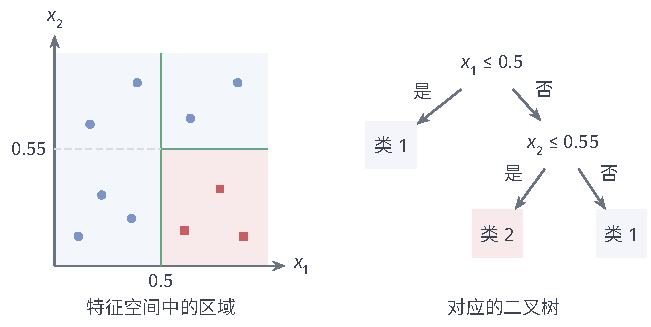
\includegraphics[width=\linewidth]{figures/03-models/01-classic-models/tikz/classification-tree-partition/figure.pdf}
  \caption{二维分类的教学构造。左图为归一化特征空间$[0,1]^2$中的区域划分，圆点表示类1，方点表示类2；右图为产生同一划分的条件树。根节点检查$x_1\leq0.5$，仅在其“否”分支上继续检查$x_2\leq0.55$。点的位置与分裂阈值均为人为设定，不代表真实数据实验。}
  \label{fig:classification-tree-partition}
\end{figure}

不同树算法的主要差异落在三个问题上：怎样评价一次分裂，允许什么样的分支结构，怎样控制树的大小。ID3提供了信息增益驱动的基本构造，C4.5扩展其评分和数据处理方式；CART则采用统一的二叉划分与子树选择框架，形成了另一条决策树研究路线。

\subsection{ID3}
\label{sec:classification-id3}

要决定先检查哪个特征，需要比较“检查前还分不清多少类别”和“检查后还分不清多少类别”。ID3（Iterative Dichotomiser 3）据此选择特征，再在各分支上重复同一过程。Quinlan在1986年的论文中将ID3追溯到Hunt等人的概念学习系统（Concept Learning System, CLS）：CLS向前考察若干层候选树，按测量与误分类代价选择测试；ID3则改用信息驱动的局部评价。这一变化把建树中的“先测什么”落实为当前节点上可计算的信息增益比较，并不保证整棵树最优。本节采用以离散特征、信息增益和不作后剪枝为设定的基本ID3\scite{quinlan1986trees}

\subsubsection{模型结构}
\label{sec:classification-id3-structure}

在节点样本集$D$上，记$p_c(D)$为类别$c$的样本比例。\term{熵}（entropy）用一个数概括类别分布的不确定性：节点只含一类时为零，各类越均匀，熵越大。采用以2为底的对数，
\begin{equation}
  H(D)=-\sum_{c=1}^{C}p_c(D)\log_2 p_c(D),
  \label{eq:classification-entropy}
\end{equation}
其中约定$0\log_2 0=0$。对第$j$个离散特征，令$V_j$为其可能取值集合，$D_{j,v}=\{(\bm{x}_i,y_i)\in D:x_{i,j}=v\}$。该特征的\term{信息增益}（information gain）是分裂前后熵的减少量：
\begin{equation}
  \operatorname{Gain}(D,j)
  =H(D)-\sum_{v\in V_j}\frac{|D_{j,v}|}{|D|}H(D_{j,v}).
  \label{eq:classification-information-gain}
\end{equation}
空子集对求和的贡献定义为零。这里必须按子集大小加权，否则只有一个样本的小分支会与包含大部分样本的分支同样重要。

ID3用选中的特征建立一个内部节点，每个取值对应一个分支。叶节点保存到达该处的类别计数，并通常输出多数类；类别计数相同时使用预先固定的平局规则。这样得到的是分段常值分类器：同一叶区域内的所有输入具有相同预测。叶节点也可报告类别频率，但少量样本上的频率不应被直接理解为可靠的概率估计。

\subsubsection{参数学习}
\label{sec:classification-id3-learning}

从根节点的$D_n$出发，算法计算所有可用特征的信息增益，选择最大者，再分别对其子集递归建树。离散特征已经按取值完全展开后，同一路径上不必再次使用它。若当前样本全部同类，就生成该类叶节点；若可用特征耗尽而标签仍不一致，就输出当前多数类。对训练时未出现的分支，可以保留以父节点多数类为输出的回退叶节点，使预测规则对新输入仍有定义。

每次选择只依据当前节点，因而这是\term{贪心搜索}（greedy search）：接受眼前收益最大的分裂，不回头枚举所有可能的整棵树。基本ID3不在建树后再作剪枝；限制最大深度、最小叶样本数或最小增益，属于另外加入的生长控制。尤其是“增益为零就停止”也会改变基本搜索行为：在异或关系中，单个特征的增益可能为零，而连续两次测试可以完全分开类别。停止规则既能减少无效分裂，也可能阻止发现特征交互。

\subsubsection{小结}
\label{sec:classification-id3-summary}

信息增益把分裂选择变成了可计算的局部比较，却有\term{多值偏差}（multivalued attribute bias）：取值很多的特征更容易把训练样本分成纯净的小组。若每条记录的编号都不同，用编号分裂会使所有子节点熵为零，增益达到$H(D)$，但对一个新编号几乎没有帮助。再加上基本ID3缺少后剪枝，训练集中的噪声也可能变成专门的叶节点。

ID3因此适合说明树怎样从样本中长出来，却不能仅凭训练误差小就获得泛化保证。接下来的C4.5分别处理评分偏差、输入类型和树的规模，保留的仍是这种递归划分思想。

\subsection{C4.5}
\label{sec:classification-c45}

让决策树用于含连续数值和缺失字段的数据，除了换一个分裂分数，还需要约定阈值怎样选择、未知值怎样传递、哪些枝条应当删除。Quinlan在1993年的专著中给出了C4.5的完整程序体系。它沿用ID3的递归构造，同时加入增益率、连续特征测试、缺失值处理、错误估计剪枝和规则提取\scite{quinlan1993c45}

\subsubsection{模型结构}
\label{sec:classification-c45-structure}

多值特征容易得到大增益，是因为它本身就把数据切得很细。C4.5用\term{信息增益率}（gain ratio）比较“类别信息的增加”与“产生这些分支所需的划分信息”。设测试$a$把$D$分成$D_1,\ldots,D_b$，令$q_v=|D_v|/|D|$，则
\begin{align}
  \operatorname{SplitInfo}(D,a)
  &=-\sum_{v=1}^{b}q_v\log_2 q_v,
  \label{eq:classification-split-information}\\
  \operatorname{GainRatio}(D,a)
  &=\frac{\operatorname{Gain}(D,a)}
  {\operatorname{SplitInfo}(D,a)}.
  \label{eq:classification-gain-ratio}
\end{align}
这里的信息增益仍按式\eqref{eq:classification-information-gain}计算，只把按特征取值划分替换为测试$a$的各个结果。分母为零意味着没有真正划分，不能参与比值比较。

归一化并未消除所有问题。若某个测试只分离出极少数样本，其划分信息也很小，微小的增益可能被除法放大。因此，C4.5不是在所有测试中直接取增益率最大者，而是先计算候选测试的平均信息增益，只在增益不低于该平均值的测试中比较增益率。这个筛选避免纯粹依靠小分母取胜；它是启发式约束，并不保证每次都选中最有泛化价值的特征。

\subsubsection{参数学习}
\label{sec:classification-c45-learning}

离散特征可以按取值作多路分裂；连续特征则使用$x_j\leq t$与$x_j>t$的二路测试。候选阈值来自排序后相邻不同取值之间，且分裂后必须满足最小子节点样本量等限制。连续特征在某次分裂后仍可在后代节点使用，因为同一数值轴上可能需要多个阈值。

C4.5各版本对阈值的评价略有区别。较早版本按增益率选择阈值；Quinlan在1996年的修订中先按信息增益选择连续特征的阈值，再扣除搜索阈值所需的描述长度代价，参与特征之间的增益筛选和增益率比较。若有$q$个候选切分位置，这项逐样本惩罚形如$\log_2 q/|D|$，用来抵消“可试阈值更多”带来的选择优势。算法~\ref{alg:classification-c45}突出这些版本共有的建树骨架，把阈值评价留在候选测试生成步骤中\scite{quinlan1996continuous}

\begin{algorithm}[C4.5的递归生长与后剪枝]
  \label{alg:classification-c45}
  \begin{algorithmic}[1]
    \Require 节点样本$D$，可用特征集合$F$，停止及剪枝设置
    \Ensure 剪枝后的分类树
    \Function{Grow}{$D,F$}
      \If{$D$全部同类，或样本量不足，或$F$为空}
        \State \Return 以$D$中多数类为输出的叶节点
      \EndIf
      \State 生成各特征的有效测试，连续特征同时选择阈值
      \State 计算各测试的增益；缺失值按正文约定处理
      \If{没有有效测试，或最大增益不为正}
        \State \Return 以$D$中多数类为输出的叶节点
      \EndIf
      \State 求候选测试的平均增益$\bar g$
      \State 保留增益不低于$\bar g$且划分信息为正的测试
      \State 选择其中增益率最大的测试$a$，建立节点$T$
      \For{测试$a$的每个结果$v$}
        \State 得到相应的子集$D_v$及子问题的特征集合$F_v$
        \If{$D_v$为空}
          \State 将$D$的多数类叶节点接到分支$v$
        \Else
          \State 将$\Call{Grow}{D_v,F_v}$接到分支$v$
        \EndIf
      \EndFor
      \State \Return $T$
    \EndFunction
    \State $T\gets\Call{Grow}{D,F}$
    \State 自底向上比较子树与简化方案的悲观错误估计
    \State \Return 剪枝后的$T$
  \end{algorithmic}
\end{algorithm}

缺失值不能简单地当作已知测试结果。设测试$a$的已知样本总权重占当前节点的比例为$q_{\mathrm{known}}$。C4.5在这些已知样本上估计类别熵的下降，再乘$q_{\mathrm{known}}$降低证据不足的测试所得收益；划分信息还计入未知部分的比例。选定测试后，把缺失该特征的样本按已知样本进入各分支的比例作分数权重分配。后续熵、类别计数和多数类都相应使用权重。预测时遇到缺失值，也按分支权重综合子树的类别预测，而不是随意选一条路径。

树生长完成后，C4.5采用\term{悲观错误剪枝}（pessimistic error pruning）：训练误差倾向于低估新样本错误，因而以二项错误计数的上置信估计作修正，比较保留子树与折叠成多数类叶节点的估计错误数。若简化方案不更差，就可以删除该子树；完整实现还可考察用某个子树提升替代当前分支。置信设置控制剪枝强度，但这种在自适应建树后使用的错误估计是模型选择启发式，不能直接当作整棵树泛化误差的严格置信保证。

树也可以转成规则：每条根到叶路径的测试构成规则前件，叶类别作为后件，再尝试删除不必要条件并筛选规则。未经简化的路径规则继承树的区域划分；条件删除以后可能产生重叠，因此规则系统还必须规定冲突处理和默认预测。这种转换并非只把树的文字抄成一份无序清单。

\subsubsection{小结}
\label{sec:classification-c45-summary}

C4.5对ID3的扩展相互配合：增益筛选和增益率调整局部测试的比较，阈值及缺失值机制扩大可处理的数据范围，后剪枝和规则简化控制最终结构的复杂度。它适合需要检查预测条件的任务，但实际可读性仍取决于树深、规则数和特征含义。单棵树与支持向量机或提升树谁更准确，需要在相同数据划分和调参预算下比较，不能仅由算法名称决定。

\subsection{CART}
\label{sec:classification-cart}

另一种组织树的方法是把每次测试都限定成二选一，再统一研究大树中应保留哪些子树。\term{分类与回归树}（classification and regression trees, CART）采用这一框架；Breiman、Friedman、Olshen与Stone在1984年的专著中将树的构造、最优剪枝与统计性质放在同一体系中讨论。其中，代价复杂度剪枝把“怎样长出一棵大树”与“最终保留多大的子树”分开：生长阶段比较局部分裂，剪枝阶段形成候选子树序列，再用验证选择规模。因此，CART与ID3的区别不只是换一个不纯度指标，还涉及分支结构与整树选择。这里关注分类树；第\ref{sec:regression-cart}节的回归CART复用递归二分与代价复杂度剪枝，但按响应损失选择分裂并在叶内输出数值，本节则按类别不纯度或误分类代价分裂并输出类别标签或类别比例\scite{breiman1984cart}

\subsubsection{模型结构}
\label{sec:classification-cart-structure}

CART分类树通常用\term{基尼不纯度}（Gini impurity）评价节点中类别的混杂程度：
\begin{equation}
  G(D)=1-\sum_{c=1}^{C}p_c(D)^2.
  \label{eq:classification-gini}
\end{equation}
它也等于从节点经验类别分布独立抽取两个标签时，两者不同的概率。对于产生左右子集$D_{\mathrm{L}}$和$D_{\mathrm{R}}$的测试$a$，比较
\begin{equation}
  \Delta G(D,a)=G(D)
  -\sum_{v\in\{\mathrm{L},\mathrm{R}\}}
  \frac{|D_v|}{|D|}G(D_v).
  \label{eq:classification-gini-decrease}
\end{equation}
基尼与熵都鼓励子节点变纯，但并不总给出相同的排序。基尼省去了对数运算，也不意味着整个训练必然更快，因为阈值搜索和数据访问可能占用更多时间。

对连续特征，二分测试仍是阈值比较；对类别特征，测试可写成$x_j\in S$与$x_j\notin S$，其中$S$是部分取值组成的集合。寻找这个集合本身也是搜索问题，取值很多时不能假定枚举所有分组都很便宜。统一的二叉结构便于遍历和剪枝，但可能用多层测试表达一棵多路树的一次分裂。

\subsubsection{参数学习}
\label{sec:classification-cart-learning}

生长阶段反复选择基尼下降最大的有效二分测试，直到满足生长限制，得到一棵较大的树$T_0$。随后进行\term{代价复杂度剪枝}（cost-complexity pruning）：不再逐个比较局部增益，而是在$T_0$的候选子树中平衡拟合误差和叶节点数。令$L(T)$为树$T$的叶节点集合，$\hat c_\ell$为叶$\ell$的预测类别，定义
\begin{align}
  \widehat R(T)
  &=\frac{1}{n}\sum_{\ell\in L(T)}
    \sum_{(\bm{x}_i,y_i)\in D_\ell}
    \mathbb{1}\{y_i\neq\hat c_\ell\},
  \label{eq:classification-cart-empirical-risk}\\
  J_\alpha(T)&=\widehat R(T)+\alpha|L(T)|,
  \qquad \alpha\geq0.
  \label{eq:classification-cart-cost-complexity}
\end{align}
这里$\widehat R(T)$采用全训练集上的误分类比例，使不同子树的误差具有共同尺度。有些软件把叶不纯度的加权和作为剪枝代价；使用其参数时需要核对具体定义，而不能混用不同尺度的$\alpha$。

剪枝路径可以由\term{最弱环节剪枝}（weakest-link pruning）生成。设内部节点$t$以下的子树为$T_t$，把它折叠成一个叶节点后，该区域对全训练集误差的贡献为$\widehat R(t)$；保留时贡献为$\widehat R(T_t)$。两种方案的代价相等时，
\begin{equation}
  \alpha_t=
  \frac{\widehat R(t)-\widehat R(T_t)}
       {|L(T_t)|-1}.
  \label{eq:classification-weakest-link}
\end{equation}
分子是折叠后增加的训练错误，分母是删去的叶数，因而$\alpha_t$衡量“每少保留一个叶节点要付出多少误差”。剪去最小$\alpha_t$对应的分支，再重新计算，就得到从大树到根叶节点的嵌套序列。若某些分支增加叶数却不降低误分类率，可先在$\alpha=0$时合并；临界值处可能有多个最优子树，按一致的最小子树约定处理平局。

对每个$\alpha$，上述序列包含相应的最优剪枝子树，但最优性仅限于给定$T_0$的子树，不是所有可能决策树。实际需要用验证集或交叉验证选择$\alpha$；交叉验证时，各训练折都应独立生长和剪枝，不能先用全体数据确定结构，再把同一结构放入各验证折评分。

\subsubsection{小结}
\label{sec:classification-cart-summary}

把叶节点多数类换成数值均值，把分类不纯度换成平方误差，就得到平方损失下的回归树构造；不需要另换一种树的表示。随机森林常采用这种二叉树，梯度提升方法也常用回归树拟合更新方向。不过，提升树的分裂目标可能来自所用损失的梯度与曲率，不能一概说成直接运行原始CART分类算法。

CART的经典框架还讨论了\term{替代分裂}（surrogate split），即主测试特征缺失时，寻找能够尽量复现主分裂结果的其他特征测试。类别权重和误分类代价也能改变生长与叶预测。具体软件未必实现全部机制；例如scikit-learn的决策树采用优化的CART框架，但类别特征编码和缺失值行为须以相应版本接口为准。二叉结构方便实现，不会自动消除噪声、类别不平衡或数据漂移带来的困难。

\subsection{规则分类与RIPPER}
\label{sec:classification-rules}
\label{sec:classification-ripper}

在分类任务中，规则的结论是类别标签。第\ref{sec:classic-overview-tree-rules}节已介绍规则与树的表示差别；这里采用有序规则，预测由首次命中的类别及默认类决定，训练则需要同时处理条件增长、剪枝与覆盖。

逐条学习规则时，一个直接困难是：为了覆盖少量例外，不断增加条件会产生庞大的规则集；过早删去条件，又可能丢失有用的局部结构。早期的AQ系列探索了从样本归纳条件规则的路线，后来的规则学习把覆盖策略与误差控制结合起来。Fürnkranz与Widmer在1994年提出\term{增量减错剪枝}（incremental reduced error pruning, IREP），将单条规则的增长和立即剪枝嵌入逐条学习过程，以避免先生成庞大规则集再统一简化的开销\scite{furnkranz1994irep}

Cohen在1995年改进IREP的剪枝评分和停止准则，并加入整组规则的反复优化，形成RIPPER（Repeated Incremental Pruning to Produce Error Reduction）。其核心不是保证找到全局最优规则，而是在规则长度、覆盖范围和错误之间进行可承受的启发式搜索。下面分别说明增长、剪枝、覆盖和优化在这一过程中承担什么作用\scite{cohen1995ripper}

\subsubsection{模型结构}
\label{sec:classification-ripper-structure}

RIPPER输出有序规则以及一个默认类别$c_0$。第$r$条规则的前件可写为
\begin{equation}
  a_r(\bm{x})=\bigwedge_{j=1}^{m_r}b_{r,j}(\bm{x}),
  \qquad a_r(\bm{x})\Longrightarrow y=c_r,
  \label{eq:classification-rule-form}
\end{equation}
其中$b_{r,j}$是一个返回真或假的测试，$m_r$为该规则的条件数。例如，$x_1>60$与$x_2=\text{是}$可以组成一个合取，但每个测试的业务含义必须由特征定义决定。规则\term{覆盖}（cover）样本，指样本满足其前件，与样本真实标签是否等于后件无关。

若规则数为$s$，预测时寻找最小的$r\in\{1,\ldots,s\}$使$a_r(\bm{x})$成立，输出$c_r$；不存在这样的$r$时输出$c_0$。二分类中，可以为目标类学习若干规则，把另一类作为默认类。多分类时，经典RIPPER通常按类别出现频率由低到高学习，逐次区分当前类与尚待区分的其他类，把最常见类放在默认位置。这种类别排序有助于为少数类显式生成规则，但不构成少数类召回率的保证。

\subsubsection{参数学习}
\label{sec:classification-ripper-learning}

RIPPER采用\term{顺序覆盖}（sequential covering）：在尚未被前面规则覆盖的工作集上学习一条规则，加入有序列表后，再处理没有命中的记录。设当前目标类别为$c_+$，属于该类的记录称为正例，其余为负例。保留原始二类训练集$D^{(0)}$用于整体评分，另用$U$表示不断缩小的覆盖工作集。区分这两个对象很重要：从$U$移除一条被错误覆盖的负例，并不是把这个错误从模型评价中抹去。

学习单条规则时，先分层随机划分增长集与剪枝集，经典设置约为$2:1$。增长从空前件开始，空前件覆盖所有样本；每次添加一个测试，使前件更严格、覆盖范围更小。测试可直接使用连续特征的阈值，无须一律在训练前离散化。Cohen的实现对缺失特征采用保守约定：涉及该特征的测试在缺失记录上不成立，因此规则需要其他已知字段来覆盖这些记录。

增长时使用源自FOIL（First Order Inductive Learner）的信息增益评分。设加入条件前覆盖$p_0$个正例、$q_0$个负例，加入后覆盖$p_1$个正例、$q_1$个负例，其中$q$不表示全章的样本量$n$。在命题规则设定下，评分为
\begin{equation}
  g=p_1\left(
  \log_2\frac{p_1}{p_1+q_1}
  -\log_2\frac{p_0}{p_0+q_0}
  \right).
  \label{eq:classification-foil-gain}
\end{equation}
括号比较加入条件前后的正例纯度，外面的$p_1$避免只看纯度而忽略保留下来的正例数。候选条件必须保留正例并满足覆盖量等实现约束；增长通常持续到不再覆盖增长集负例，或没有可接受的改进条件。不可分的噪声样本可能使前一种停止情形无法达到，算法不能为追求绝对纯净而无限增长。

剪枝则允许把规则末端的一串条件一起删掉，也就是比较增长过程中得到的各个前缀，而非只尝试删去一个条件。若某个前缀在剪枝集覆盖$p$个正例、$q$个负例，RIPPER的基本评分是
\begin{equation}
  v=\frac{p-q}{p+q},\qquad p+q>0.
  \label{eq:classification-ripper-pruning}
\end{equation}
在分母为正时，它与覆盖样本中的正确率$p/(p+q)$给出相同排序。剪枝选择评分最好的可接受前缀，平局可偏向较短者；覆盖不到剪枝样本时，分数没有定义，需要回退或拒绝，而不能擅自记成满分。这一评分改变了原IREP对规则的偏好，尤其避免单凭覆盖大量样本而认可纯度不足的条件。

单条规则看起来合理，也可能使整组规则过于复杂。\term{最小描述长度}（minimum description length, MDL）把这种取舍表达为：用多少比特写下规则，再用多少比特说明规则预测错了哪些训练标签。记有序规则集为$\mathcal{R}$，总描述长度可概括为
\begin{equation}
  L_{\mathrm{total}}(\mathcal{R};D^{(0)})
  =L_{\mathrm{rules}}(\mathcal{R})
   +L_{\mathrm{errors}}(D^{(0)}\mid\mathcal{R}).
  \label{eq:classification-rule-description-length}
\end{equation}
第二项按完整规则集及默认类计算，因而仍包含误覆盖记录。Cohen的实验允许总长度暂时超过此前的最小值，但超过64比特就停止增加规则，再从后向前删除会增加总长度的规则。64是实现中的停止设置，不是统计定理给出的常数，也不要求每次加规则都立即缩短总长度。

算法~\ref{alg:classification-ripper}给出二类子问题的主要流程。伪代码中的增长和剪枝采用前述评分，描述长度的编码细节由具体实现确定；多分类时在外层加入类别排序与默认类约定。

\begin{algorithm}[RIPPER的覆盖学习与规则优化]
  \label{alg:classification-ripper}
  \begin{algorithmic}[1]
    \Require 二类样本$D^{(0)}$，目标类$c_+$，优化轮数$b$
    \Ensure 有序规则集$\mathcal{R}$及默认负类
    \State $\mathcal{R}\gets()$
    \Function{Extend}{$\mathcal{R},D^{(0)}$}
      \State $U\gets D^{(0)}$中未被$\mathcal{R}$覆盖的样本
      \State $L_{\min}\gets L_{\mathrm{total}}(\mathcal{R};D^{(0)})$
      \While{$U$中仍有正例}
        \State 将$U$分层随机划为增长集$G$和剪枝集$P$
        \State 从空前件增长规则$a$，按式\eqref{eq:classification-foil-gain}添加条件
        \State 在$P$上按式\eqref{eq:classification-ripper-pruning}选择$a$的前缀
        \If{无可接受规则，或$a$不覆盖$U$中的任何正例}
          \State \textbf{停止本轮覆盖学习}
        \EndIf
        \State 把$a\Longrightarrow c_+$追加到$\mathcal{R}$
        \State $L\gets L_{\mathrm{total}}(\mathcal{R};D^{(0)})$
        \State $L_{\min}\gets\min(L_{\min},L)$
        \If{$L>L_{\min}+64$}
          \State \textbf{停止本轮覆盖学习}
        \EndIf
        \State 从$U$移除被$a$覆盖的全部样本，包括正例和负例
      \EndWhile
      \State 从后向前删除能使总描述长度降低的规则
      \State \Return $\mathcal{R}$
    \EndFunction
    \State $\mathcal{R}\gets\Call{Extend}{\mathcal{R},D^{(0)}}$
    \For{$t=1,\ldots,b$}
      \For{按顺序考察$\mathcal{R}$中的每条规则}
        \State 从空前件生成替代规则，从原前件生成修订规则
        \State 剪枝候选规则时，评价完整规则集在剪枝集上的错误
        \State 用总描述长度在原规则、替代规则、修订规则之间选择
      \EndFor
      \State $\mathcal{R}\gets\Call{Extend}{\mathcal{R},D^{(0)}}$
    \EndFor
    \State \Return $\mathcal{R}$，无规则匹配时预测负类
  \end{algorithmic}
\end{algorithm}

优化阶段是在整组规则的上下文中改写单条规则。替代规则从空前件重新增长，修订规则在原前件上继续添加条件；对候选规则的剪枝不只看它自身的纯度，还看替换后完整有序规则集的错误。随后用MDL选择保留原规则还是采用候选，必要时重新进行规则删除和剩余正例的覆盖学习。原论文把一次优化称为RIPPER，重复两次称为RIPPER2；优化次数是可配置的搜索预算，不能解释为已经完成全局最优化。

\subsubsection{小结}
\label{sec:classification-ripper-summary}

RIPPER适合需要按条件讨论预测的场景，例如审阅异常交易或核查业务规则。增长提供局部区分能力，留出剪枝降低对增长集偶然细节的依赖，覆盖避免重复处理已经命中的输入，MDL与规则优化限制整体复杂度。这些机制控制过拟合风险，但不保证在任意噪声和样本量下都得到短而准确的规则。

连续特征可由阈值直接处理；多分类和类别不平衡也不能简单归为“不支持”或“能力弱”。真正需要检查的是少数类能否在增长集与剪枝集中获得足够样本、类别排序是否合适，以及使用总体错误率会不会忽略重要的漏报。规则变多、条件变长和重叠变复杂时，预测与人工审阅的成本都会上升，不能仅凭规则形式就认为模型已经满足可审计要求。

\subsection{模型对比与总结}
\label{sec:classification-trees-comparison}
\label{sec:classification-rules-comparison}

本小节先比较ID3、C4.5与CART，再介绍改变分裂检验、工程实现或叶模型的代表性扩展。表~\ref{tab:classification-tree-comparison}按同一组问题比较三种基本方法。C4.5的主要变化是补充分裂评分、输入处理和错误估计，CART则把二叉结构与一条可验证选择的剪枝路径结合起来。两者都不能保证找到泛化误差最小的树，因而不能把一种剪枝准则描述成对另一种的无条件优越替代。

\begin{table}[htbp]
  \centering
  \small
  \begin{tabularx}{\linewidth}{@{}l*{3}{>{\RaggedRight\arraybackslash}X}@{}}
    \toprule
    方法 & 分裂评分 & 基本分支形式 & 规模控制 \\
    \midrule
    ID3 & 信息增益 & 离散取值多路分裂 & 基本版本无后剪枝 \\
    C4.5 & 增益筛选与增益率 & 离散多路、连续阈值二分 & 悲观错误估计剪枝 \\
    CART & 基尼不纯度下降 & 统一二叉分裂 & 代价复杂度路径及验证选择 \\
    \bottomrule
  \end{tabularx}
  \caption{三种决策树在基本分类设定下的比较。输入支持和停止细节随实现版本变化。}
  \label{tab:classification-tree-comparison}
\end{table}

沿着C4.5的程序体系，C5.0进一步改进树与规则生成的实现，并加入提升集成、样本权重、误分类代价和特征筛选等功能\scite{rulequest2017c50}提升集成反复学习多个分类器，改变后续学习对样本的关注，再组合各分类器的输出；AdaBoost是这一序贯重加权路线的代表构造\scite{freund1997boosting}解释集成预测时，需要同时考察多个模型。样本权重表示不同训练记录的重要性，误分类代价则区分不同错误的损失，使训练目标能够反映实际决策中的代价差异。RuleQuest提供商业版本和GPL源码版本，其公开实验报告了特定数据与硬件条件下的速度及内存改进；实际收益随数据规模、输出树还是规则集等设置变化。

若关注的不只是类别变纯，还包括分裂是否有足够的统计证据，可以采用Kass于1980年提出的\term{卡方自动交互检测}（chi-square automatic interaction detection, CHAID）。它对类别特征的取值与标签建立列联表，先合并类别分布差异不显著的取值，再比较各特征与响应的关联，按经过多重比较调整的检验结果选择分裂；证据不足时停止。剩下的取值组形成多路分支，适合把分群结果读作交叉分类，但连续变量通常需要先分组，分组方式会影响结果。这里的显著性针对相应检验的关联假设，既不是因果证据，也不能直接作为全树不出错的保证\scite{kass1980chaid}

信息增益和基尼下降还面临另一种偏差：候选切分越多，越容易偶然找到一个高分切分。\term{条件推断树}（conditional inference tree, CTree）把“选哪个特征”与“在该特征上怎样切分”分开。Hothorn、Hornik与Zeileis在2006年的框架中用条件置换分布评价特征与响应的关联：先检验当前节点中所有特征均与响应无关联的全局原假设；不能拒绝时停止，否则选择检验证据最强的特征，再为它寻找二分位置。通过同一检验尺度和多重检验控制，可以缓解不同取值数目带来的选择偏差\scite{hothorn2006ctree}

CTree的统计解释有明确边界。置换检验依赖相应原假设下的可交换性，渐近近似的可靠程度又受样本量影响；若标签与单个特征都不相关、只通过交互发生联系，节点检验也可能停止。检验驱动的生长控制为是否继续分裂提供依据，但不等于对所有分布都严格控制泛化误差，或保证小样本任务一定优于经过验证的其他树。

也可以保留树的区域划分，却改变叶节点如何预测。\term{逻辑模型树}（logistic model tree, LMT）在每个叶区域内使用Logistic回归，即用特征的线性得分表示类别对数几率，再转成类别概率。这样，树负责不同区域之间的结构变化，叶模型负责区域内部随特征变化的概率。Landwehr、Hall与Frank的2005年期刊论文基于其2003年会议工作，通过LogitBoost逐步拟合逻辑模型，并在后代节点继续细化祖先模型，而不是把每个小叶中的模型都完全独立地从零估计\scite{landwehr2005lmt}

例如在二分类叶区域$\ell$内，LMT可输出
\begin{equation}
  \hat p_\ell(y=1\mid\bm{x})
  =\frac{1}{1+\exp[-(\bm{w}_\ell^\top\bm{x}+b_\ell)]},
  \label{eq:classification-lmt-leaf}
\end{equation}
其中$\bm{w}_\ell\in\mathbb{R}^d$和$b_\ell\in\mathbb{R}$是叶模型的系数。概率在单个叶区域内部平滑变化，但跨越不同叶的边界时仍可能跳变，也不自动具有良好的校准性质。模型拟合、迭代次数选择和树剪枝共同增加训练成本，解释时也要同时阅读路径条件与叶模型系数。

这些变种分别改变分裂证据、实现或叶模型。对树结构波动的进一步处理放在第\ref{sec:classification-ensemble}节；此处的比较仍针对单棵分类树。

本小节先比较树与RIPPER的条件组织方式，再介绍单特征规则、束搜索和决策表等代表性扩展。树与规则的差别主要是条件如何共享，以及训练时怎样寻找这些条件。树在一个节点上的分裂同时决定多个分支，适合复用共同的前置判断；直接规则学习一次寻找一个局部区域，不要求不同区域具有相同的判断顺序。两者都要反复搜索，树并不是“一次训练就完成”而规则才需要迭代。若若干类别区域共享长前缀，树可能更紧凑；若局部条件各不相同，扁平规则可以避免为维持树结构而复制分支。

复杂规则学习是否真的必要，可以用只看一个特征的方法作比较。\term{单特征规则}（one rule, OneR）对每个候选特征建立“取值到多数类”的映射，再选择训练错误最少的特征。这里的“one”指一个特征：具有多个取值的特征通常对应多条if--then规则。连续特征需要形成带有最小样本量约束的区间，防止每个数值都单独成组。Holte在1993年的研究发现，在所考察的常用基准数据上，单特征规则与更复杂学习器的预测表现并不总有很大差距。这为使用简单基线检验任务难度提供了实证依据，但具体结论仍受所选数据集限制\scite{holte1993oner}

\begin{example}[一个特征可以产生多条规则]
  \label{ex:classification-oner}
  构造一个含10个样本的二分类训练集。特征$A$有$a,b,c$三个取值，对应的“类1、类2”计数分别为$(3,1)$、$(1,2)$和$(0,3)$。按每组多数类预测，得到三条规则：$A=a$时判为类1，$A=b$或$A=c$时分别判为类2，训练错误数为$1+1+0=2$。另一个二值特征$B$的两组计数均为$(2,3)$，其单特征映射的错误数为$2+2=4$。OneR在这两个候选中选择$A$，得到的是一个特征上的三条取值规则。新记录出现未见取值时，仍需要预先约定多数类回退等处理方式。
\end{example}

若一个特征不够，又希望在条件搜索中保留多种可能，可以采用Clark与Niblett于1989年提出的CN2。它结合AQ的规则覆盖思想与类似ID3的纯度评价，用\term{束搜索}（beam search）寻找条件合取：每轮扩展已有候选，只保留评分最好的$b$个候选继续搜索，其中$b$为束宽。相较于只保留一个候选，束搜索能探索更多路径，但被舍弃的条件仍可能属于最优规则，因此并不保证避开局部最优。CN2还用显著性筛选限制偶然形成的纯净小区域\scite{clark1989cn2}

原始CN2学习有序规则，Clark与Boswell在1991年的改进中进一步研究了无序规则：针对类别分别生成条件，允许多个规则共同参与预测。有序规则以首次命中解决冲突；无序规则则需要组合匹配规则的类别分布或投票权重。无序表示减少了对单一顺序的依赖，却把解释负担转移到重叠和冲突处理上，因此规则学习和预测时的聚合约定需要配套选择\scite{clark1991cn2}

规则还可以组织成查找表。\term{决策表}（decision table）选择一个特征子集$S\subseteq\{1,\ldots,d\}$，把训练样本在这些特征上的取值组合作为键，保存同键样本的多数类。训练的难点主要转向选择$S$：特征太少会把不同类别混在一起，特征太多又使组合稀疏、难以匹配新样本。Kohavi在1995年研究了通过特征子集搜索学习决策表的方法，使用验证误差评价候选组合；最佳优先搜索不断扩展当前较好的候选子集，并在若干次扩展没有改善时停止，而不是保证遍历全部子集\scite{kohavi1995decisiontable}

决策表通常只保存训练中实际出现的组合，不必枚举所有理论上可能的取值。连续值需要离散化或另外约定匹配方法，未出现的组合可回退到训练多数类。在哈希索引下，查表本身可以很快，但还要读取并构造包含$|S|$个特征的键，特征搜索的训练代价也不能忽略。它适合可用少量离散字段表达的决策；若类别由复杂交互决定，表会变大，且相近却不完全相同的输入不能自动共享统计证据。

OneR限制使用的特征数，CN2扩大条件搜索范围，RIPPER交替覆盖、剪枝和优化，决策表则共享一组索引特征。这些方法是在不同位置限制模型复杂度，不是一条规则越来越细就必然越来越准确的路线。选择时应同时检查独立验证误差、规则规模、未匹配输入和冲突处理；只有这些行为都明确，规则形式才真正有助于使用和审阅。

\section{基于概率的分类}
\label{sec:classification-probability}

第\ref{sec:classic-overview-probabilistic}节已区分直接建立条件类别概率与先描述类条件输入分布的两条路线。本节分别用Logistic回归、朴素贝叶斯和GDA说明参数估计、类别决策与概率检验。沿用训练集$D_n$，类别数为$C$、类别索引为$c$；$p$按观测类型表示概率质量函数或概率密度。LDA的共享协方差推导见第\ref{sec:classification-lda}节，这里直接在一般高斯模型族中使用该结果。

\subsection{Logistic 回归}
\label{sec:classification-logistic}

若直接用实值线性函数拟合$0/1$标签，输出可能小于零或大于一，不能直接解释为概率。\term{Logistic回归}（logistic regression）保留线性得分，却通过一个有界变换把它映射为正类概率。这里将二分类标签约定为$\{0,1\}$；名称中的“回归”描述对概率与特征关系的建模，任务仍是分类。

第\ref{sec:regression-glm}节把伯努利分布、logit链接与其他响应模型统一在广义线性模型中；本节复用这套条件概率结构，但进一步规定类别决策阈值与误判代价，并单独检查概率校准。

Logistic曲线的历史早于统计分类。Verhulst在1838年用它描述受增长上限约束的人口变化，后来这一曲线进入生物测定和二值响应分析。从增长曲线到统计回归，函数保留了相同形式，变量与参数的解释却发生了变化；Cramer对这一发展过程作了专门考证\scite{cramer2002origins}

\subsubsection{模型结构}
\label{sec:classification-logistic-structure}

记$p(\bm{x})=\mathbb{P}(y=1\mid\bm{x})$。比值$p(\bm{x})/[1-p(\bm{x})]$称为\term{几率}（odds），衡量正类相对于负类的可能性。对它取对数得到\term{对数几率}（log-odds，也称logit），其取值可以覆盖整个实数轴，因而适合与线性得分连接：
\begin{equation}
  \label{eq:classification-logistic-logodds}
  \log\frac{p(\bm{x})}{1-p(\bm{x})}
  =\bm{w}^{\top}\bm{x}+b.
\end{equation}
其中$\bm{w}\in\mathbb{R}^{d}$是权重，$b\in\mathbb{R}$是偏置。令右侧为$z$，由$p/(1-p)=e^z$整理出$p=e^z/(1+e^z)$，便得到
\begin{equation}
  \label{eq:classification-logistic-sigmoid}
  p(\bm{x})=\sigma(\bm{w}^{\top}\bm{x}+b),
  \qquad
  \sigma(z)=\frac{1}{1+e^{-z}}.
\end{equation}
这个S形函数称为\term{Sigmoid函数}（sigmoid function），此处特指Logistic形式。它把任意有限得分转成严格介于零和一之间的数。Cox在1958年的二值序列回归研究是这一统计建模路线的经典文献\scite{cox1958binary}

参数的解释落在对数几率尺度上：保持其他特征不变，$x_j$增加一个单位，正类几率乘以$e^{w_j}$。概率本身的变化还取决于原来的概率，因为
\[
  \frac{\partial p(\bm{x})}{\partial x_j}
  =w_jp(\bm{x})[1-p(\bm{x})].
\]
因此，$w_j$的正负说明模型中的影响方向，大小却不能脱离特征单位直接比较，也不自动具有因果含义。例如，假设某特征的$w_j=\log 2$，原来正类概率为$1/2$，该特征增加一单位后概率变为$2/3$，而不是增加固定的$\log 2$。

在两类误判代价相同时，以$p(\bm{x})\geq1/2$预测正类，边界就是$\bm{w}^{\top}\bm{x}+b=0$。若误报的代价为$a>0$、漏报为$r>0$，正确分类代价为零，则预测正类的条件是$a[1-p(\bm{x})]\leq rp(\bm{x})$，即阈值改为$a/(a+r)$。这一决策解释要求输入概率足够可靠；合法的数值范围本身还不能保证这一点。

图\ref{fig:classification-logistic-probability}把概率阈值与得分阈值放在同一条曲线上比较。一般地，概率阈值$\tau\in(0,1)$对应得分阈值$\log[\tau/(1-\tau)]$。在图中的教学设定下，误报与漏报代价相等时取$\tau=0.5$；若改成$a=4$、$r=1$，则$\tau=0.8$，得分至少达到$\log4\approx1.386$才预测正类。曲线本身没有改变，改变的是把概率转成类别的规则。
\begin{figure}[htbp]
  \centering
  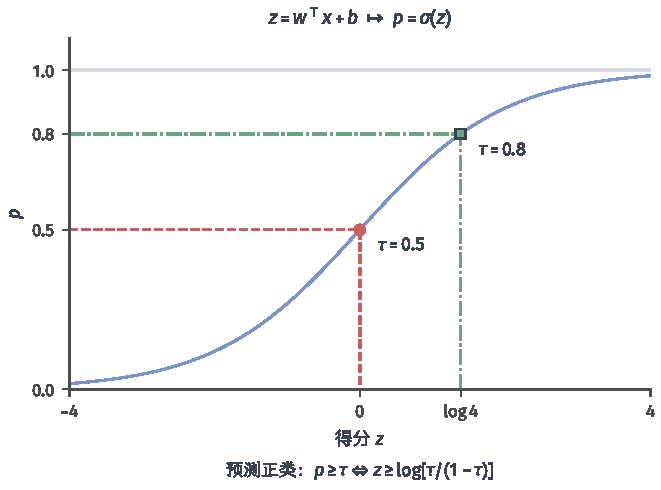
\includegraphics[width=\linewidth]{figures/03-models/01-classic-models/matplotlib/classification-logistic-probability/figure.pdf}
  \caption{线性得分$z=\bm{w}^{\top}\bm{x}+b$经Logistic函数转为正类概率$p$。蓝色实线为$p=\sigma(z)$；红色虚线与圆点标出$(0,0.5)$，绿色点划线与方点标出$(\log4,0.8)$。两组辅助线分别连接概率阈值与对应的得分阈值，数值是教学构造，不表示训练或校准结果。}
  \label{fig:classification-logistic-probability}
\end{figure}

\subsubsection{参数学习}
\label{sec:classification-logistic-learning}

对独立样本，模型给出的标签概率为$p_i^{y_i}(1-p_i)^{1-y_i}$，其中$p_i=\sigma(\bm{w}^{\top}\bm{x}_i+b)$。\term{最大似然估计}（maximum likelihood estimation, MLE）选择使已观察标签最可能出现的参数。其条件对数似然为
\begin{equation}
  \label{eq:classification-logistic-likelihood}
  \ell(\bm{w},b)
  =\sum_{i=1}^{n}
  \bigl[y_i\log p_i+(1-y_i)\log(1-p_i)\bigr].
\end{equation}
最大化$\ell$等价于最小化负对数似然$L=-\ell$，也就是二分类\term{交叉熵损失}（cross-entropy loss）：给真实标签分配的概率越低，惩罚越大。令增广输入$\tilde{\bm{x}}_i=(\bm{x}_i^{\top},1)^{\top}$、参数$\bm{\beta}=(\bm{w}^{\top},b)^{\top}\in\mathbb{R}^{d+1}$，并记$z_i=\tilde{\bm{x}}_i^{\top}\bm{\beta}$，可写成
\begin{equation}
  \label{eq:classification-logistic-loss}
  L(\bm{\beta})
  =\sum_{i=1}^{n}\bigl[\log(1+e^{z_i})-y_i z_i\bigr].
\end{equation}
数值计算不宜先求极端概率再取对数，可用$\log(1+e^z)=\max\{0,z\}+\log(1+e^{-|z|})$避免指数溢出。

为确定更新方向，利用$\sigma'(z)=\sigma(z)[1-\sigma(z)]$求导。令$\tilde{\bm{X}}\in\mathbb{R}^{n\times(d+1)}$的第$i$行为$\tilde{\bm{x}}_i^{\top}$，$\bm{p}=(p_1,\ldots,p_n)^{\top}$、$\bm{y}=(y_1,\ldots,y_n)^{\top}$，则
\begin{equation}
  \label{eq:classification-logistic-derivatives}
  \begin{aligned}
    \nabla L(\bm{\beta})
      &=\tilde{\bm{X}}^{\top}(\bm{p}-\bm{y}),\\
    \nabla^2 L(\bm{\beta})
      &=\tilde{\bm{X}}^{\top}\bm{R}\tilde{\bm{X}},\\
    \bm{R}
      &=\operatorname{diag}\bigl(p_i(1-p_i)\bigr)_{i=1}^{n}.
  \end{aligned}
\end{equation}
梯度中的$p_i-y_i$是预测概率与观察标签的差。对任意$\bm{v}\in\mathbb{R}^{d+1}$，Hessian的二次型为
\[
  \bm{v}^{\top}\nabla^2L\,\bm{v}
  =\sum_{i=1}^{n}p_i(1-p_i)
    (\tilde{\bm{x}}_i^{\top}\bm{v})^2\geq0.
\]
所以负对数似然$L$是凸函数，而被最大化的$\ell$是凹函数。有限参数处的$p_i(1-p_i)>0$；若$\tilde{\bm{X}}$列满秩，$L$严格凸，否则可能存在不改变训练得分的平坦方向。这涉及\term{可识别性}（identifiability）：数据能否区分不同参数。即使严格凸，也只能保证有限极小点若存在便唯一，不能保证它一定存在。

例如，若存在$\bm{\beta}_0$使$(2y_i-1)\tilde{\bm{x}}_i^{\top}\bm{\beta}_0>0$对所有样本成立，沿$t\bm{\beta}_0$令$t\to\infty$，每项损失均趋于零，但任意有限$t$的损失仍大于零。完全分离的数据因此没有有限MLE；准完全分离也可能使部分参数发散。完整的存在性分析区分分离、准分离和重叠情形，不能仅凭凸性断言“唯一全局最优解”\scite{albert1984existence}

实际训练常加入$\lambda\lVert\bm{w}\rVert_2^2/2$，其中$\lambda>0$。这个$L_2$惩罚抑制权重无限增大，也改善病态方向的数值条件。若两类均有样本，所有权重都受惩罚而偏置不受惩罚，所得二分类目标仍有唯一有限极小点；但若训练集只有一类，偏置仍可独自趋于无穷。若连偏置也作正的二次惩罚，则整个增广参数方向都受约束。使用$\lambda\lVert\bm{w}\rVert_1$可得到稀疏权重，但目标不再处处可微，不能直接套用下面的光滑牛顿更新。

求解器的选择取决于数据规模和存储成本。稠密数据的一轮完整梯度计算为$O(nd)$，构造Hessian约为$O(nd^2)$，直接分解又需要$O(d^3)$。若存储$d\times d$量级的Hessian过于昂贵，\term{有限内存拟牛顿法}（limited-memory BFGS, L-BFGS）只保留少量历史更新来近似二阶信息。大规模稀疏数据则可采用\term{随机梯度下降}（stochastic gradient descent, SGD），每次用一个样本或小批量近似完整梯度。选择时还应考虑稀疏程度和精度要求，而不是固定的样本数门槛。

数据持续到达时，也可以增量更新模型。McMahan等人的点击率系统使用稀疏正则与在线优化，展示了Logistic回归在大规模预测中的工程用途\scite{mcmahan2013}增量训练省去了每次从头拟合的成本，但持续更新能否改善未来预测，仍取决于更新规则和数据变化。

对于中小规模问题，\term{迭代重加权最小二乘}（iteratively reweighted least squares, IRLS）把牛顿步改写为一个权重随当前预测变化的最小二乘问题。令$\bm{J}=\operatorname{diag}(1,\ldots,1,0)$，使偏置不受惩罚。在第$t$步计算
\begin{equation}
  \label{eq:classification-logistic-irls}
  \begin{aligned}
    u_i^{(t)}
      &=z_i^{(t)}
        +\frac{y_i-p_i^{(t)}}{p_i^{(t)}(1-p_i^{(t)})},\\
    \bm{\beta}^{(t+1)}
      &\in\argmin_{\bm{\beta}}\left\{
        \begin{aligned}
          &\frac12\sum_{i=1}^{n}\bm{R}_{i,i}^{(t)}
            (u_i^{(t)}-\tilde{\bm{x}}_i^{\top}\bm{\beta})^2\\
          &\quad{}+\frac{\lambda}{2}
            \bm{\beta}^{\top}\bm{J}\bm{\beta}
        \end{aligned}
      \right\}.
  \end{aligned}
\end{equation}
这里的$u_i^{(t)}$是供当前二次近似使用的工作响应，不是新标签。对应正规方程为
\[
  \bigl(\tilde{\bm{X}}^{\top}\bm{R}^{(t)}\tilde{\bm{X}}
       +\lambda\bm{J}\bigr)\bm{\beta}^{(t+1)}
  =\tilde{\bm{X}}^{\top}\bm{R}^{(t)}\bm{u}^{(t)}.
\]
将$\bm{u}^{(t)}$代入即可还原“当前参数减去Hessian逆作用于梯度”的牛顿步。实现时应解线性方程而不显式求逆，并用阻尼或线搜索控制更新；当$p_i$接近零或一时，直接计算工作响应可能不稳定，可改用梯度与Hessian求牛顿方向。停止条件可综合梯度范数、目标变化与最大迭代次数，牛顿法的局部快速收敛不意味着从任意初始化都可无阻尼运行\scite{hastie2009}

\subsubsection{支持多分类（Softmax）}
\label{sec:classification-logistic-softmax}

新闻主题等任务要求在$C$个互斥类别中选择一个，不能把每一类都当成互不相关的二分类输出。\term{Softmax回归}（softmax regression，也称multinomial logistic regression）同时建立各类得分，并将它们转成总和为一的概率；它保留的是“任意两类的对数概率比为线性函数”这一结构。

\textbf{模型结构。}为每类引入$\bm{w}_c\in\mathbb{R}^{d}$和$b_c\in\mathbb{R}$，令$z_c(\bm{x})=\bm{w}_c^{\top}\bm{x}+b_c$。其后验模型为
\begin{equation}
  \label{eq:classification-softmax-model}
  p_c(\bm{x})
  =\mathbb{P}(y=c\mid\bm{x})
  =\frac{\exp z_c(\bm{x})}
         {\sum_{r=1}^{C}\exp z_r(\bm{x})}.
\end{equation}
指数保证概率为正，分母保证归一化；两类之间的分母相消，得到
\[
  \log\frac{p_c(\bm{x})}{p_r(\bm{x})}
  =(\bm{w}_c-\bm{w}_r)^{\top}\bm{x}+b_c-b_r.
\]
当$C=2$时，$p_1(\bm{x})=\sigma((\bm{w}_1-\bm{w}_2)^{\top}\bm{x}+b_1-b_2)$。把第1类视为正类、第2类视为负类，就回到二分类Logistic回归。

共同增加得分不会改变概率。更具体地，对任意$\bm{a}\in\mathbb{R}^{d}$和$t\in\mathbb{R}$，变换$\bm{w}_c\mapsto\bm{w}_c+\bm{a}$、$b_c\mapsto b_c+t$使每个指数项同乘$\exp(\bm{a}^{\top}\bm{x}+t)$，因而全部约掉。这是$d+1$维的参数冗余。选择第$C$类为\term{参考类}（reference class），就是把该类完整的增广参数固定为零：
\begin{equation}
  \label{eq:classification-softmax-reference}
  \begin{gathered}
    \bm{w}_C=\bm{0},\qquad b_C=0,\\
    \log\frac{p_c(\bm{x})}{p_C(\bm{x})}
    =\bm{w}_c^{\top}\bm{x}+b_c
    \quad(c<C).
  \end{gathered}
\end{equation}
仅固定$\bm{w}_C$而不固定$b_C$不够。类似地，$\lambda\sum_c\lVert\bm{w}_c\rVert_2^2/2$能够消除共同权重平移的自由，却不能锁定共同偏置平移；仍须约束偏置，例如令$\sum_c b_c=0$，或惩罚全部偏置。消除这种固有冗余后，还应检查训练设计矩阵的秩与数据分离，不能把这些不同问题混为一谈。

\textbf{参数学习。}现在$y_i\in\{1,\ldots,C\}$，记$p_{i,c}=p_c(\bm{x}_i)$，$\bm{\Theta}\in\mathbb{R}^{(d+1)\times C}$的第$c$列为$\bm{\beta}_c=(\bm{w}_c^{\top},b_c)^{\top}$。多类负对数似然是
\begin{equation}
  \label{eq:classification-softmax-loss}
  \begin{aligned}
    L(\bm{\Theta})
      &=-\sum_{i=1}^{n}\log p_{i,y_i}\\
      &=\sum_{i=1}^{n}\left[
        \log\sum_{c=1}^{C}e^{z_c(\bm{x}_i)}
        -z_{y_i}(\bm{x}_i)\right].
  \end{aligned}
\end{equation}
以$\mathbb{1}\{\cdot\}$表示条件成立时为一、否则为零的指示函数，梯度为
\begin{equation}
  \label{eq:classification-softmax-gradient}
  \begin{aligned}
    \nabla_{\bm{w}_c}L
      &=\sum_{i=1}^{n}
        [p_{i,c}-\mathbb{1}\{y_i=c\}]\bm{x}_i,\\
    \frac{\partial L}{\partial b_c}
      &=\sum_{i=1}^{n}
        [p_{i,c}-\mathbb{1}\{y_i=c\}].
  \end{aligned}
\end{equation}
它仍由“预测减观察”的残差驱动。Hessian的$(c,r)$参数块为
\[
  \nabla^2_{\bm{\beta}_c,\bm{\beta}_r}L
  =\sum_{i=1}^{n}p_{i,c}
    [\mathbb{1}\{c=r\}-p_{i,r}]
    \tilde{\bm{x}}_i\tilde{\bm{x}}_i^{\top}.
\]
对任意增广参数扰动$\bm{v}_c$，令$a_{i,c}=\tilde{\bm{x}}_i^{\top}\bm{v}_c$，相应二次型为
\[
  \sum_{i=1}^{n}\left[
    \sum_{c=1}^{C}p_{i,c}a_{i,c}^2
    -\left(\sum_{c=1}^{C}p_{i,c}a_{i,c}\right)^2
  \right]\geq0.
\]
方括号正是以$\bm{p}_i$为权重的方差，故$L$凸。共同平移使方差为零，秩亏还会引入其他平坦方向；分离数据上同样可能不存在有限MLE。参考类约束解决表示冗余，适当正则化控制参数大小，两者的作用不同。

Softmax可用分块牛顿法、L-BFGS或小批量SGD优化，多类Hessian还包含类别间的耦合，不能简单把$C$个独立的二分类IRLS问题拼起来。求概率时应先减去$m(\bm{x})=\max_c z_c(\bm{x})$，用$e^{z_c-m}/\sum_r e^{z_r-m}$得到完全相同且更稳定的结果。普通稠密实现的一轮梯度计算约为$O(ndC)$。

类别特别多时，分母求和也会成为瓶颈。\term{层次Softmax}（hierarchical softmax）以树上路径概率的乘积替代平坦分类参数化；\term{噪声对比估计}（noise-contrastive estimation, NCE）通过区分数据与人为噪声来估计模型；\term{负采样}（negative sampling）只对抽取的负例建立局部区分目标。三者都可减少某些计算，但不能统称为原Softmax似然的等价计算，尤其负采样通常改变了训练目标\scite{goodfellow2016}

\textbf{决策与概率语义。}预测可取$\hat y(\bm{x})=\argmax_c p_c(\bm{x})=\argmax_c z_c(\bm{x})$，并按固定类别次序处理平局。Softmax输出已经满足概率公理，却不自动满足\term{概率校准}（probability calibration）：在被预测为某类概率约为$0.8$的样本中，该类的实际比例也应接近$0.8$。有限样本、模型失配、正则化和分布变化都可能破坏这种对应。

Softmax常用作神经网络的分类输出层，但其归一化也不能保证整个网络校准。Guo等对现代网络的实验表明，分类准确与置信度可靠可以明显分离；独立验证数据上的温度缩放等方法能改善一些设置下的校准，却仍不是任意新分布下的保证\scite{guo2017calibration}

\subsubsection{小结}
\label{sec:classification-logistic-summary}

Logistic回归把线性得分、条件概率与代价敏感阈值连接起来，多类版本则用Softmax联合比较各类。固定特征表示下的训练目标凸，便于优化与复核；权重也可在对数几率尺度上解释。但可识别性、有限解的存在性和概率校准分别需要检查，不能从“凸目标”或“概率输出”一并推出。

它的表示限制来自线性对数几率：若需要非线性交互，应显式加入交叉项或其他特征变换。训练可通过随机优化增量进行，预测则只需保存参数并计算得分。信用评分、医学风险预测和点击率预估都可以采用这种基线，但具体特征与验证方式需要对应到各自任务。

\subsection{朴素贝叶斯}
\label{sec:classification-naive-bayes}

若希望通过“哪一类更可能产生当前输入”来分类，就需要估计类条件分布。困难在于，$d$个二值特征已有$2^d$种组合，逐一统计需要大量样本。\term{朴素贝叶斯}（naive Bayes, NB）把复杂的联合分布拆成较小的分布，用简化假设换取少量统计量和直接的参数估计。这样的约束可能降低有限样本下的估计波动，也可能引入持续的模型偏差，并不无条件提高精度。

Maron在1961年关于自动索引的研究，是概率方法用于文档归类的早期工作之一。文档分类需要从大量词项中提取可累积的类别证据，这也成为朴素贝叶斯的一项典型用途\scite{maron1961indexing}

\subsubsection{模型结构}
\label{sec:classification-naive-bayes-structure}

对一般特征向量，NB采用给定类别后的\term{条件独立}（conditional independence）假设：已知$y=c$后，一个特征的取值不再改变其他特征的分布。令$\pi_c=\mathbb{P}(y=c)$、$p_{j,c}(x_j)=p(x_j\mid y=c)$，模型写成
\begin{equation}
  \label{eq:classification-naive-bayes-model}
  \begin{aligned}
    q_c(\bm{x})&=\prod_{j=1}^{d}p_{j,c}(x_j),\\
    \mathbb{P}_{\mathrm{NB}}(y=c\mid\bm{x})
      &=\frac{\pi_c q_c(\bm{x})}
      {\sum_{r=1}^{C}\pi_r q_r(\bm{x})}.
  \end{aligned}
\end{equation}
记号$q_c$强调这是模型使用的乘积分布，未必等于真实类条件分布。条件独立不要求全部训练样本混在一起时特征仍独立，例如词项之间的总体相关性可能部分来自主题差异。

只需要分类时，各类共同的分母可以省略。为避免许多小概率连乘下溢，通常比较对数得分
\begin{equation}
  \label{eq:classification-naive-bayes-score}
  s_c(\bm{x})
  =\log\pi_c+\sum_{j=1}^{d}\log p_{j,c}(x_j),
  \qquad
  \hat y(\bm{x})=\argmax_c s_c(\bm{x}).
\end{equation}
这里$s_c$不是归一化的对数后验；需要概率时还须减去$\log\sum_r e^{s_r}$。零概率可使得分为负无穷，后面的平滑正是为未见事件保留概率质量。文档的多项式版本沿用相似得分，但它的独立性对象是词元位置，而非总长度固定后的各维计数，必须另外说明。

\subsubsection{参数学习}
\label{sec:classification-naive-bayes-learning}

令$n_c=\sum_i\mathbb{1}\{y_i=c\}$，类先验的MLE为$\hat\pi_c=n_c/n$。这是以训练样本的类别比例估计目标总体的比例，依赖抽样具有代表性；若训练集人为重采样，不能未经修正就把重采样后的比例当成部署先验。也可以使用有依据的外部类别比例；若希望保留对该比例的不确定性，并为训练中未见的类别保留概率质量，则可对类概率向量$\bm{\pi}=(\pi_1,\ldots,\pi_C)^{\top}$设置参数先验。以下对类别概率与各组类条件参数设置相互独立的先验，以便分别更新。

使用\BookSectionRef{sec:probability-common-distributions}{第一卷“数学准备”的常见分布模型小节}
中的\term{Dirichlet分布}，给类概率向量设置正参数$\gamma_c$的先验。
独立类别记录的计数进入各坐标的幂次，因而
\[
  \begin{aligned}
    p(\bm{\pi})
      &\propto\prod_{c=1}^{C}\pi_c^{\gamma_c-1},\\
    p(y_1,\ldots,y_n\mid\bm{\pi})
      &\propto\prod_{c=1}^{C}\pi_c^{n_c},\\
    p(\bm{\pi}\mid y_1,\ldots,y_n)
      &\propto\prod_{c=1}^{C}\pi_c^{\gamma_c+n_c-1}.
  \end{aligned}
\]
后验仍是Dirichlet分布，只需把参数从$\gamma_c$更新为$\gamma_c+n_c$。
这种先验与后验属于同一分布族的关系称为\term{共轭}（conjugacy）。
使用卷一的均值公式，后验均值为
\[
  \tilde\pi_c=\frac{n_c+\gamma_c}
  {n+\sum_{r=1}^{C}\gamma_r}.
\]
先验均值为$\gamma_c/\sum_r\gamma_r$，参数总和决定这些伪计数相对于观测计数的权重。这里“类别先验$\pi_c$”是样本生成模型的一部分，“参数先验”则表达估计$\bm{\pi}$前的不确定性，两者不是同一个概率。

连续特征可采用\term{高斯朴素贝叶斯}（Gaussian naive Bayes），即$x_j\mid y=c\sim\mathcal{N}(\mu_{j,c},\sigma_{j,c}^{2})$，其中$\sigma_{j,c}^{2}>0$。当$n_c>0$且该特征的类内平方偏差和为正时，均值和方差的MLE为
\begin{equation}
  \label{eq:classification-naive-bayes-gaussian}
  \begin{aligned}
    \hat\mu_{j,c}
      &=\frac{1}{n_c}\sum_{i:y_i=c}x_{i,j},\\
    \hat\sigma_{j,c}^{2}
      &=\frac{1}{n_c}\sum_{i:y_i=c}
        (x_{i,j}-\hat\mu_{j,c})^2.
  \end{aligned}
\end{equation}
方差分母为$n_c$，不是无偏样本方差所用的$n_c-1$。在上述条件下，预测时将这些量代入一维高斯密度后相乘。若某类某特征恒定为$a$，固定$\mu_{j,c}=a$后，对数似然为$-n_c\log(2\pi\sigma_{j,c}^{2})/2$，随正方差趋于零而无界增大。因此，此时正方差参数域内没有有限MLE；式\eqref{eq:classification-naive-bayes-gaussian}给出的零值只是样本散度，不能代入普通高斯密度。设定有明确尺度的方差下限或加入先验后，得到的是相应的受约束或正则化估计；给密度任意“加一”不是离散概率的平滑对应物。

只关心某个词是否出现时，可用\term{伯努利朴素贝叶斯}（Bernoulli naive Bayes）。输入$x_{i,j}\in\{0,1\}$，令$n_{j,c}=\sum_{i:y_i=c}x_{i,j}$，则
\begin{equation}
  \label{eq:classification-naive-bayes-bernoulli}
  \begin{aligned}
    q_c(\bm{x})
      &=\prod_{j=1}^{d}
        \theta_{j,c}^{x_j}(1-\theta_{j,c})^{1-x_j},\\
    \hat\theta_{j,c}&=\frac{n_{j,c}}{n_c}.
  \end{aligned}
\end{equation}
未出现的词同样提供证据，不能只保留$x_j=1$的项；这里的MLE要求$n_c>0$。
为平滑这个二值事件，使用卷一的Beta分布作为$\theta_{j,c}$的先验，
两个正参数$\alpha_1,\alpha_0$分别对应出现与未出现。乘以似然后，
两项指数分别增加$n_{j,c}$和$n_c-n_{j,c}$，所以
\[
  \theta_{j,c}\mid D_n
  \sim\operatorname{Beta}
    (\alpha_1+n_{j,c},\,\alpha_0+n_c-n_{j,c}).
\]
其后验均值为$(n_{j,c}+\alpha_1)/(n_c+\alpha_1+\alpha_0)$；对称情形$\alpha_1=\alpha_0=\alpha$的分母是$n_c+2\alpha$。这同时平滑了出现和未出现两种事件。

若重复出现的次数也有意义，应使用\term{多项式朴素贝叶斯}（multinomial naive Bayes）。设固定词表有$d$个词项，$\bm{x}_i\in\mathbb{N}_0^d$记录一篇文档的词项计数，$m_i=\sum_jx_{i,j}$是该文档的总词元数。给定类别和$m_i$，假设每个词元位置独立地按$\bm{\theta}_c=(\theta_{1,c},\ldots,\theta_{d,c})^{\top}$抽取词项，其中$\sum_j\theta_{j,c}=1$。忽略顺序后，计数向量服从
\begin{equation}
  \label{eq:classification-naive-bayes-multinomial}
  \mathbb{P}(\bm{x}_i\mid y_i=c,m_i)
  =\frac{m_i!}{\prod_{j=1}^{d}x_{i,j}!}
    \prod_{j=1}^{d}\theta_{j,c}^{x_{i,j}}.
\end{equation}
因为计数总和已固定，各维计数并不独立。将它写成每维整数取值的独立类别分布，会改变模型和分母。McCallum与Nigam专门比较了伯努利和多项式这两种文档事件模型，明确区分“词是否出现”与“词出现多少次”\scite{mccallum1998event}

标准文档分类通常进一步假设长度分布与类别无关，因而$\mathbb{P}(m_i\mid y_i=c)$在类别比较中约掉，此时给定长度后的类先验仍为$\pi_c$。若长度本身携带类别信息，则应保留并估计该项，使长度也参与后验计算。

令$t_{j,c}=\sum_{i:y_i=c}x_{i,j}$为第$c$类中词项$j$的总出现次数，$t_c=\sum_jt_{j,c}$为该类的总词元数。去掉与参数无关的组合系数后，类内对数似然为$\sum_jt_{j,c}\log\theta_{j,c}$。当$t_c>0$时，在$\sum_j\theta_{j,c}=1$约束下求极值，正计数坐标上的拉格朗日方程给出$t_{j,c}/\theta_{j,c}$为同一常数，零计数坐标取零；求和确定常数为$t_c$，从而得到频率MLE。

若对$\bm{\theta}_c$使用$\operatorname{Dirichlet}(\alpha_1,\ldots,\alpha_d)$先验，其中$\alpha_j>0$，同样的共轭更新把各坐标的幂次从$\alpha_j-1$变为$\alpha_j+t_{j,c}-1$，得到
\[
  \bm{\theta}_c\mid D_n
  \sim\operatorname{Dirichlet}
    (\alpha_1+t_{1,c},\ldots,\alpha_d+t_{d,c}).
\]
把更新后的参数归一化即可得到后验均值。两种估计分别为
\begin{equation}
  \label{eq:classification-naive-bayes-smoothing}
  \hat\theta_{j,c}=\frac{t_{j,c}}{t_c},
  \qquad
  \tilde\theta_{j,c}
  =\frac{t_{j,c}+\alpha_j}
         {t_c+\sum_{r=1}^{d}\alpha_r}.
\end{equation}
前式要求$t_c>0$；后式也给出下一词元的后验预测概率，因为给定参数时该概率为$\theta_{j,c}$，对参数后验积分便得到其后验均值。这种均值估计通常既不同于MLE，也不同于式\eqref{eq:regression-map}定义的MAP。对称$\alpha_j=1$给出\term{拉普拉斯平滑}（Laplace smoothing），相当于每个词项加入一个伪计数；$\alpha_j=1/2$对应多项式参数的Jeffreys先验。对伯努利参数，其对应物是$\operatorname{Beta}(1/2,1/2)$，不应把这些常数不加区分地推广到高斯方差。以平滑估计代入式\eqref{eq:classification-naive-bayes-multinomial}得到的是常用的点估计分类器，不等于积分消去参数后的整篇文档预测分布。

在长度与类别无关的约定下，文档预测只需计算$\log\tilde\pi_c+\sum_jx_j\log\tilde\theta_{j,c}$。算法\ref{alg:classification-multinomial-nb}给出完整的统计与预测流程，训练和预测使用相同的词表，并明确处理平滑与得分平局。
\begin{algorithm}[带平滑的多项式朴素贝叶斯]
  \label{alg:classification-multinomial-nb}
  \begin{algorithmic}[1]
    \Require 非空训练集$D_n$，固定词表大小$d$与类别数$C$；
    \Statex \hspace{\algorithmicindent} 词项伪计数$\alpha>0$，类别伪计数$\gamma>0$
    \Ensure 类先验$\tilde{\bm{\pi}}$、词项概率$\tilde{\bm{\Theta}}$及预测规则
    \State 检查所有输入为有限非负整数计数，标签属于$\{1,\ldots,C\}$
    \State 将$n_c$、$t_c$与$t_{j,c}$全部初始化为零
    \For{$i=1,\ldots,n$}
      \State 令$c=y_i$，并更新$n_c\gets n_c+1$
      \For{满足$x_{i,j}>0$的词项$j$}
        \State $t_{j,c}\gets t_{j,c}+x_{i,j}$
        \State $t_c\gets t_c+x_{i,j}$
      \EndFor
    \EndFor
    \For{$c=1,\ldots,C$}
      \State $\tilde\pi_c\gets(n_c+\gamma)/(n+C\gamma)$
      \State 对所有$j$，令$\tilde\theta_{j,c}\gets(t_{j,c}+\alpha)/(t_c+d\alpha)$
    \EndFor
    \State 对新计数向量$\bm{x}$，按相同词表与输入检查计算
    \Statex \hspace{\algorithmicindent}
      $s_c=\log\tilde\pi_c+\sum_{j:x_j>0}x_j\log\tilde\theta_{j,c}$
    \State 返回$s_c$最大的类别；平局时返回索引最小的类别
  \end{algorithmic}
\end{algorithm}

假设词表只有三个词项，两类累计计数分别为$(3,1,0)$和$(0,1,3)$，类先验均为$1/2$。取$\alpha=1$，平滑后的词项概率分别为$(4,2,1)/7$和$(1,2,4)/7$。对新文档$\bm{x}=(1,0,1)^{\top}$，两类乘积相同，判决平局；对$\bm{x}=(2,0,1)^{\top}$，两类得分之差为$\log4$，于是选择第1类。这个教学例子显示了重复计数怎样改变证据，而零计数词项经平滑后不会把整类概率直接清零。

\subsubsection{理论分析}
\label{sec:classification-naive-bayes-theory}

\paragraph{收敛性分析}
NB的计数估计有闭式表达式，这里的收敛问题不是迭代优化何时停止，而是样本增加后估计量趋向什么。固定特征维数、类别数和有限取值集合，在独立同分布抽样且各类先验为正时，强大数定律保证经验类频率和类内相对频率几乎必然收敛到对应的真实概率。固定伪计数相对于不断增长的类内样本数趋于零，因此不改变这一极限。

单维条件概率估计一致，并不要求同一样本的各维特征条件独立；但把这些概率相乘后能否还原真实联合分布，需要额外的模型假设。高斯NB若要一致地估计类条件密度，还要求高斯族正确、方差非退化并使用一致估计。多项式NB则要求词元生成与长度处理假设正确，训练文档的抽样及总计数满足相应大数定律。有限离散情形的频率收敛证明包含在下面的风险一致性证明中。

\paragraph{泛化分析}
估计量收敛后，还需回答由这些估计构造的分类器能否接近贝叶斯风险。下面先在模型正确的有限离散情形下给出完整证明，再考察条件独立不成立时，哪些依赖会改变决策。这个结论描述样本数趋于无穷时的风险，不是有限样本的误差上界，也无需排除后验平局。
\begin{theorem}[有限离散特征下NB的风险一致性]
  \label{thm:classification-naive-bayes-consistency}
  设$d$、$C$固定，每维特征的取值集合有限，训练样本独立同分布，且每类先验$\pi_c>0$。若真实分布满足给定类别后的特征条件独立，使用经验类频率与类内相对频率估计概率，或加入固定的正伪计数，则所得NB分类器$\hat h_n$满足
  \[
    R(\hat h_n)\longrightarrow R^\ast
    \quad\text{几乎必然}.
  \]
  这里$R(h)=\mathbb{P}(h(\bm{X})\neq Y)$针对独立的新样本计算，$R^\ast$为贝叶斯风险；几乎必然收敛针对无限训练样本序列。早期若$n_c=0$，可任意指定该类的条件分布；若某输入的全部类别得分为零，也可任意指定该处的预测。
\end{theorem}
\begin{proof}
  对取值$v$及$n_c>0$的类别，类内估计为
  \[
    \hat p_{j,c}(v)
    =\frac{\sum_{i=1}^{n}\mathbb{1}\{x_{i,j}=v,y_i=c\}}
           {n_c}.
  \]
  由强大数定律，$n_c/n\to\pi_c>0$，故空类别事件几乎必然最终不再出现。分子除以$n$收敛到$\mathbb{P}(X_j=v,Y=c)$，因此$\hat p_{j,c}(v)\to p_{j,c}(v)$几乎必然。固定伪计数相对于$n_c$趋于零，不改变极限。有限多个估计可同时收敛；对每个$\mathbb{P}(\bm{X}=\bm{x})>0$的输入，归一化分母最终为正，早期任意约定不影响极限。乘积与归一化于是给出
  \[
    \hat\eta_{n,c}(\bm{x})
    \longrightarrow
    \eta_c(\bm{x})=\mathbb{P}(Y=c\mid\bm{X}=\bm{x}).
  \]
  令$c^\ast$最大化真实后验，$\hat c$最大化估计后验。因为$\hat\eta_{n,\hat c}\geq\hat\eta_{n,c^\ast}$，插入这两个估计值得到
  \[
    0\leq\eta_{c^\ast}(\bm{x})-\eta_{\hat c}(\bm{x})
    \leq2\max_c|\hat\eta_{n,c}(\bm{x})-\eta_c(\bm{x})|.
  \]
  左侧就是该输入处的超额分类风险。对有限个输入按真实概率加权求和，右侧趋于零，故整体风险趋于$R^\ast$。
\end{proof}

后验平局时，最大化类别可能随$n$变化，但选择不同的最优类别并不增加风险。因此，风险一致性不等于决策最终处处固定，更不能由“依概率收敛”直接推出无条件的决策几乎必然一致。若模型失配，估计可能稳定地收敛到不同于真实联合分布的乘积分布；增加样本能减小估计误差，却不会自动消除这种模型偏差。

真实数据中的词语、测量量和相邻像素常有依赖，但违反独立性并不直接决定分类误差。Domingos与Pazzani在1997年的研究区分了概率估计误差与零一分类损失，报告了含依赖数据上的经验结果，并在特定条件下分析了合取、析取概念等情形的最优性。分类只要求最高得分类别正确，因此概率估计失真与分类仍然准确可以同时发生\scite{domingos1997optimality}

为拆开这些层次，暂取二分类$c\in\{0,1\}$，并使用真实类先验与真实单维条件分布构造总体NB，不含有限样本估计误差。在下列分母均为正的输入处，定义
\begin{equation}
  \label{eq:classification-naive-bayes-ratios}
  \begin{aligned}
    r(\bm{x})
      &=\frac{\pi_1p(\bm{x}\mid y=1)}
              {\pi_0p(\bm{x}\mid y=0)},\\
    r_{\mathrm{NB}}(\bm{x})
      &=\frac{\pi_1\prod_jp(x_j\mid y=1)}
              {\pi_0\prod_jp(x_j\mid y=0)}.
  \end{aligned}
\end{equation}
若平局都归第1类，则两个分类器在该输入上的决策相同，当且仅当$r\geq1$与$r_{\mathrm{NB}}\geq1$同真同假。理由只是：用正的第0类联合得分除两边，不改变类别得分的大小关系。这是从判决规则直接得到的等价关系，不是对NB有效范围的独立保证；其中$r$还是未知真分布的量。

要解释依赖何时不会改变比值，可以进一步定义
\begin{equation}
  \label{eq:classification-naive-bayes-dependence}
  \begin{aligned}
    a_c(\bm{x})
      &=\frac{p(\bm{x}\mid y=c)}
              {\prod_{j=1}^{d}p(x_j\mid y=c)},\\
    r(\bm{x})
      &=r_{\mathrm{NB}}(\bm{x})
        \frac{a_1(\bm{x})}{a_0(\bm{x})}.
  \end{aligned}
\end{equation}
$a_c$衡量真实联合分布相对于乘积分布的修正。条件独立使$a_c=1$；更弱的充分条件是$a_1=a_0>0$，此时即使两类内部都有依赖，其修正在类别比值中也完全相消。由概率链式法则还可写成
\[
  a_c(\bm{x})
  =\prod_{j=1}^{d}
    \frac{p(x_j\mid x_1,\ldots,x_{j-1},y=c)}
         {p(x_j\mid y=c)}.
\]
各因子不必分别为一，不同位置的修正也可在整体乘积中抵消。所需比较的是两类中这些概率修正的比值，而不只是通常的相关系数。Zhang在2004年以局部依赖比和全局依赖分布因子展开了这一思路\scite{zhang2004optimality}

完全相消仍只是充分条件。若$r_{\mathrm{NB}}\neq1$，且
\[
  \left|\log a_1(\bm{x})-\log a_0(\bm{x})\right|
  <\left|\log r_{\mathrm{NB}}(\bm{x})\right|,
\]
则修正不足以改变对数比的正负，决策仍然相同。反之，依赖影响在两类中不均衡时就可能越过边界。例如把一个有信息的二值特征原样复制一次，在等类先验下，NB把原似然比平方：原比值为4时，真实后验为$4/5$，NB却报$16/17$，分类未变而置信度偏高。非等先验下，特征证据被重复计算还可能改变类别，这说明同一个依赖错误对概率与决策的影响可以不同。

\subsubsection{小结}
\label{sec:classification-naive-bayes-summary}

NB的计算优势来自统计量可累积：稠密输入的训练统计约为$O(nd)$，存储为$O(Cd)$，单样本预测为$O(Cd)$，这些量级以每维分布的参数个数有界为前提。以$\bm{X}\in\mathbb{R}^{n\times d}$记训练输入矩阵，多项式模型可按非零计数累积，训练约为$O(n+\operatorname{nnz}(\bm{X})+Cd)$，预测约为$O(C(1+\operatorname{nnz}(\bm{x})))$。这里$\operatorname{nnz}$表示非零元素数；“扫描一次”不意味着与样本数、特征数和类别数都无关。

它适合建立文档、垃圾邮件和情感分类的低成本基线，也容易增量更新。Graham在2002年8月的《A Plan for Spam》中介绍了基于词项统计的邮件过滤实践；该方法还加入词项筛选与经验修正，与本节的标准多项式模型有所不同\scite{graham2002spam}

使用NB时要分别检查输入的事件模型、特征依赖和概率校准。相关性可能造成证据重复计算，却不必然破坏分类；连续特征还可能因所选单维分布失配而出错。若业务需要可靠概率，应另用留出数据评估和校准，而不只报告准确率。

\subsection{高斯判别分析（GDA）}
\label{sec:classification-gda}

高斯NB只保存每维的均值与方差，相当于把类内协方差矩阵的非对角元素设为零。若分类信息恰好体现在多个连续特征的共同变化中，就需要估计这些关系。\term{高斯判别分析}（Gaussian discriminant analysis, GDA）用每类的多元高斯分布描述输入，允许保留类内协方差；增加的表达能力也意味着需要估计更多参数。

第\ref{sec:clustering-gmm}节的高斯混合模型同样估计高斯成分及其权重，但成分归属是潜变量，通常用\term{期望最大化}（expectation-maximization, EM）交替计算成分归属的后验概率并更新分布参数；两步计算的分类实例见第\ref{sec:classification-semisupervised-comparison}节。GDA中的类别标签已经观测，可以直接按类分组估计。两者共享高斯密度结构，却分别服务于预设类别预测和无标签分组。

从类间分离程度转向概率决策，关注的问题也从“怎样区分类别”扩展为“怎样权衡误判”。Anderson在1951年的多元分类研究中，以误分类代价为依据讨论分类规则，并在正态总体下给出判别函数。这为理解GDA提供了一条历史线索：分布模型负责描述输入来自各类的可能性，决策规则再据此比较误判代价，而不只是寻找一个投影方向\scite{anderson1951classification}

\subsubsection{模型结构}
\label{sec:classification-gda-structure}

本节用GDA统称各类具有高斯条件分布的判别模型，并分别讨论共享协方差与类特有协方差。对第$c$类，参数是$\pi_c$、$\bm{\mu}_c\in\mathbb{R}^{d}$及对称正定的$\bm{\Sigma}_c\in\mathbb{R}^{d\times d}$：
\begin{equation}
  \label{eq:classification-gda-density}
  \begin{aligned}
    p(\bm{x}\mid y=c)
      &=\frac{\exp[-\Delta_c(\bm{x})/2]}
        {(2\pi)^{d/2}|\bm{\Sigma}_c|^{1/2}},\\
    \Delta_c(\bm{x})
      &=(\bm{x}-\bm{\mu}_c)^{\top}
        \bm{\Sigma}_c^{-1}(\bm{x}-\bm{\mu}_c).
  \end{aligned}
\end{equation}
这里的二次型$\Delta_c$按类内变化尺度衡量输入偏离均值的程度；行列式项则补偿分布体积，不能在不同协方差的类别比较中丢掉。贝叶斯后验仍为$\pi_cp(\bm{x}\mid y=c)/\sum_r\pi_rp(\bm{x}\mid y=r)$。

取对数并删除所有类别共有的$-d\log(2\pi)/2$，得到判别得分
\begin{equation}
  \label{eq:classification-gda-score}
  g_c(\bm{x})
  =\log\pi_c-\frac12\log|\bm{\Sigma}_c|
   -\frac12\Delta_c(\bm{x}).
\end{equation}
预测选择最大$g_c$。这一模型不要求各特征独立，但要求整类分布可由单个多元高斯刻画；“保留完整协方差”只是保留全部二阶关系，不是能表达任意非线性依赖或多峰结构。

\subsubsection{参数学习}
\label{sec:classification-gda-learning}

有标签时，各类样本的归属已知，联合对数似然可按类别分开优化。当每类都有样本且类内散度矩阵正定时，MLE为
\begin{equation}
  \label{eq:classification-gda-estimates}
  \begin{aligned}
    \hat\pi_c&=\frac{n_c}{n},\\
    \hat{\bm{\mu}}_c
      &=\frac{1}{n_c}\sum_{i:y_i=c}\bm{x}_i,\\
    \hat{\bm{\Sigma}}_c
      &=\frac{1}{n_c}\sum_{i:y_i=c}
        (\bm{x}_i-\hat{\bm{\mu}}_c)
        (\bm{x}_i-\hat{\bm{\mu}}_c)^{\top}.
  \end{aligned}
\end{equation}
均值来自使类内平方偏差最小的驻点，协方差来自似然中的对数行列式与二次型之间的平衡。和高斯NB一样，这里使用MLE分母$n_c$；若改用$n_c-1$，得到的是无偏协方差估计。若类内散度奇异，沿未被样本覆盖的方向收缩方差可使似然不断增大，在协方差正定的参数域内没有有限MLE；此时上式的奇异矩阵只能作为样本散度统计，不能当成合法的普通高斯协方差。

共享协方差特例的完整推导已经放在第\ref{sec:classification-lda}节。简要地说，约束$\bm{\Sigma}_c=\bm{\Sigma}$后，合并类内散度给出式~\eqref{eq:classification-lda-covariance}~的MLE；展开高斯得分时，各类共有的$\bm{x}^{\top}\bm{\Sigma}^{-1}\bm{x}$相消，得到式~\eqref{eq:classification-lda-score}~的线性得分。两类得分相等因而给出超平面。若协方差随类变化，二次项一般不能约掉，得到QDA及通常为二次曲面的两类边界。共享与否改变的不是贝叶斯规则，而是允许的分布族及由此得到的得分形式\scite{bishop2006}

图\ref{fig:classification-gaussian-boundaries}在同一个二维教学例子中比较两种协方差设定。两图都取$\pi_1=\pi_2=1/2$、$\bm{\mu}_1=(-1,0)^{\top}$、$\bm{\mu}_2=(1,0)^{\top}$，坐标为无量纲特征。左图共享$\bm{\Sigma}_1=\bm{\Sigma}_2=\bm{I}_2$；右图只将第2类改为$\bm{\Sigma}_2=\operatorname{diag}(1,4)$。代入式\eqref{eq:classification-gda-score}，得分差分别为
\begin{equation}
  \label{eq:classification-gda-boundary-example}
  \begin{aligned}
    g_2-g_1&=2x_1
      &&\text{（共享协方差）},\\
    g_2-g_1&=2x_1+\frac38x_2^2-\log2
      &&\text{（类特有协方差）}.
  \end{aligned}
\end{equation}
令得分差为零，得到直线$x_1=0$和抛物线$x_1=\frac12\log2-\frac{3}{16}x_2^2$。在两种设定中，边界右侧的$g_2$都更大，预测第2类。右图中，第2类沿$x_2$方向更分散：在$x_2=0$附近，行列式项降低了它的密度峰值，边界向右移到$x_1\approx0.347$；随着$|x_2|$增大，第2类较慢衰减的密度又使其预测区域向左延伸。只看均值之间的距离，会漏掉方差尺度和密度归一化对判决的共同影响。
\begin{figure*}[htbp]
  \centering
  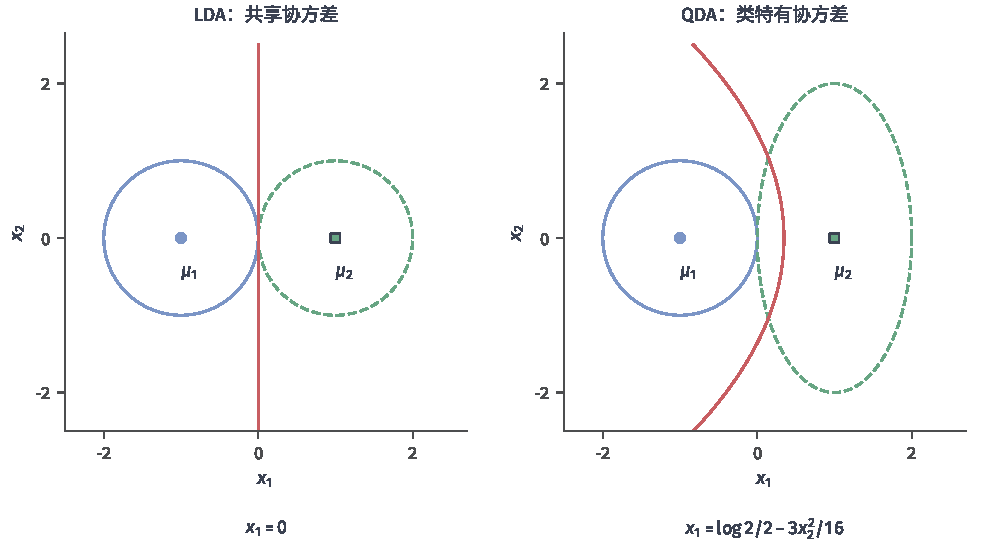
\includegraphics[width=\linewidth]{figures/03-models/01-classic-models/matplotlib/classification-gaussian-boundaries/figure.pdf}
  \caption{两图均取$\pi_1=\pi_2=1/2$、$\bm{\mu}_1=(-1,0)^{\top}$、$\bm{\mu}_2=(1,0)^{\top}$和$\bm{\Sigma}_1=\bm{I}_2$，仅第2类协方差变化。蓝色圆点和绿色方点为均值，蓝色实线与绿色虚线分别为$\Delta_1=1$和$\Delta_2=1$的等密度轮廓；不同类的这些轮廓不保证密度值相同。红色粗线按$g_1=g_2$的解析式绘制，底部公式分别给出LDA的线性边界与QDA的二次边界。参数均为教学构造，不是采样或拟合结果。}
  \label{fig:classification-gaussian-boundaries}
\end{figure*}

对二分类，把式~\eqref{eq:classification-lda-score}~中的两类得分相减并归一化，就得到Logistic形式的后验。因此，共享高斯假设蕴含线性对数几率，反过来却不成立；许多非高斯输入分布也能有Logistic形式的条件概率。即便两条路线的后验形式相同，用联合似然估计均值和协方差，与直接最大化条件似然，也通常得到不同的有限样本参数。

完整协方差每类需要$d(d+1)/2$个自由参数。类内散布矩阵的秩至多为$n_c-1$，因而$n_c\leq d$时必然奇异，不能直接代入普通高斯密度；$n_c>d$也不保证估计准确或条件良好。共享估计的秩至多为$n-C$。在维数较大或类别样本少时，可以共享、取对角，或采用
\[
  \tilde{\bm{\Sigma}}_c
  =(1-\rho)\hat{\bm{\Sigma}}_c+\rho\tau\bm{I}_d,
  \qquad 0<\rho\leq1,\quad\tau>0
\]
这样的收缩估计。$\tau$提供方差尺度，$\rho$控制偏离样本协方差的程度；这是改变估计准则，不再是未经约束的MLE。

稠密完整协方差的统计成本约为$O(nd^2)$，各类矩阵分解约为$O(Cd^3)$，存储为$O(Cd^2)$，QDA单样本得分约为$O(Cd^2)$。LDA只需分解一份协方差，并可预先算出线性权重，使单样本预测降到$O(Cd)$。实现时可用Cholesky分解求解二次型与对数行列式，无须显式构造逆矩阵。

\subsubsection{小结}
\label{sec:classification-gda-summary}

GDA用同一套生成式模型连接高斯NB、LDA与QDA：对角协方差忽略类内相关，共享协方差降低估计负担，类特有完整协方差则允许更灵活的边界。三者的选择要结合每类样本量、维数和类内结构，而不是只看总样本数。

偏离高斯假设会使密度模型失配，但不意味着分类性能必然崩塌；只要相关区域的类别得分排序仍然合理，分类仍可能有效。多峰结构、异常值和病态协方差则是需要特别检查的情形。低维连续数据可把共享或正则化GDA作为基线，同时与判别式模型比较错误率和概率质量，不能仅凭正态性检验决定胜负。

\subsection{模型对比与总结}
\label{sec:classification-probability-comparison}

本小节先比较Logistic回归、朴素贝叶斯与GDA，再介绍补集统计和放宽条件独立性的代表性扩展。这几种模型并不能沿“假设越来越强”排成一条直线。Logistic回归限制后验的对数几率形式，却不限制输入边缘分布；NB限制给定类别后的依赖结构，还要选择单维或词元的事件模型；GDA限制整体分布为高斯，但可保留NB忽略的协方差。只有指定具体模型族，例如共享协方差GDA与线性Logistic回归，才能准确讨论假设的包含关系。

表\ref{tab:classification-probability-comparison}汇总相同监督分类任务下的主要取舍。参数量按每维分布参数有界计算，GDA的共享与类特有协方差分别列明，避免把两者的代价混在一起。
\begin{table}[htbp]
  \centering
  \small
  \begin{tabularx}{\linewidth}{@{}
    >{\RaggedRight\arraybackslash}p{0.19\linewidth}
    >{\RaggedRight\arraybackslash}X
    >{\RaggedRight\arraybackslash}X@{}}
    \toprule
    模型 & 建模与估计 & 主要取舍 \\
    \midrule
    Logistic回归／Softmax回归 &
    直接拟合条件概率；$O(Cd)$个参数，迭代优化 &
    不拟合输入分布；需检查特征表示、分离与正则化 \\
    NB &
    由先验和简化类条件模型形成后验；通常$O(Cd)$个参数 &
    计数或矩估计易累积；依赖和事件模型失配会引入偏差 \\
    共享GDA（LDA） &
    高斯类条件分布，共享协方差；$O(d^2+Cd)$个参数 &
    用共同协方差降低估计波动；只得到线性边界 \\
    类特有GDA（QDA） &
    各类独立估计协方差；$O(Cd^2)$个参数 &
    边界更灵活；对每类样本量和协方差条件更敏感 \\
    \bottomrule
  \end{tabularx}
  \caption{概率分类模型的建模对象与估计代价。所有概率输出都需单独检查校准，参数量不直接等于达到指定精度所需的样本量。}
  \label{tab:classification-probability-comparison}
\end{table}

生成式与判别式方法的样本效率比较，还必须分清“较快接近自己的极限误差”与“达到同一个目标误差”。Ng和Jordan在NIPS 2001会议、2002年出版的论文中，重点比较离散NB以及共享对角方差的连续NB，与相应的Logistic回归／线性分类方法。他们分析并观察到两种可能的学习阶段：NB较快接近自身的极限误差，而判别式方法在数据更多时可能达到更低的误差。结论取决于所比较的模型与分布条件，一般完整协方差GDA不在这一结论的直接适用范围内\scite{ng2001}

其分析中，一定概率或方差下界保证参数估计受控，还需要关于决策边界附近概率质量的条件，才能把参数误差转成分类风险误差。文中的一些形式化判别结论针对在线性分类器中最小化零一风险，而不能未经额外论证就替换为交叉熵极小化。由此得到的模型选择原则是：比较学习曲线、极限偏差和实际目标损失，而不是从“生成式”三个字推出统一的速度优势。

对文本数据，除了增加训练样本，还可以调整参数的统计来源。\term{补集朴素贝叶斯}（complement naive Bayes, CNB）用不属于第$c$类的文档构造补集分布，再寻找与该补集不匹配的输入。Rennie等在2003年提出这一方法，针对类别不平衡时的权重估计偏差，并结合其他修正研究文本分类效果\scite{rennie2003complement}

沿用多项式计数，令$t_{j,\bar c}=\sum_{i:y_i\neq c}x_{i,j}$、$t_{\bar c}=\sum_jt_{j,\bar c}$。先定义补集词项参数及其对数权重：
\begin{equation}
  \label{eq:classification-complement-nb}
  \begin{aligned}
    \tilde\theta_{j,\bar c}
      &=\frac{t_{j,\bar c}+\alpha_j}
              {t_{\bar c}+\sum_{r=1}^{d}\alpha_r},\\
    w_{j,c}&=\log\tilde\theta_{j,\bar c},\\
    s_c^{\mathrm{CNB}}(\bm{x})
      &=\log\pi_c-\sum_{j=1}^{d}x_jw_{j,c}.
  \end{aligned}
\end{equation}
Rennie等给出的CNB规则选择最大$s_c^{\mathrm{CNB}}$；他们同时说明实验中为简化采用均匀类别先验，此时等价于选择补集对数得分$\sum_jx_jw_{j,c}$最小的类别。负号使“不像补集”转化为支持第$c$类的证据：$\tilde\theta_{j,\bar c}$表示补集的词项参数，与正类$\mathbb{P}(\bm{x}\mid y=c)$中的参数是不同对象。补集可能混合多个类别，本身也未必是单一多项式分布，因此CNB更适合解释为基于补集统计构造的分类得分，而不是原NB正类后验的替代估计。

同一论文还把权重归一化作为另一项修正，得到WCNB：
\[
  \bar w_{j,c}
  =\frac{w_{j,c}}{\sum_{r=1}^{d}|w_{r,c}|},
  \qquad
  \hat y(\bm{x})
  =\argmin_c\sum_{j=1}^{d}x_j\bar w_{j,c}.
\]
论文完整算法还组合了词频、逆文档频率和文档长度变换，不能把式~\eqref{eq:classification-complement-nb}、WCNB或包含全部变换的版本写成唯一的CNB形式。

常用库实现也有明确取舍。scikit-learn的\code{ComplementNB}在多类情形不使用类别先验，当前默认\code{norm=False}，即预测时比较未作第二次归一化的$-\sum_jx_j\log\tilde\theta_{j,\bar c}$；设置\code{norm=True}才启用上述权重归一化\scite{sklearnComplementNB}因此，默认实现既不同于带非均匀$\pi_c$的式~\eqref{eq:classification-complement-nb}，也不同于原论文包含权重归一化的完整算法。补集计数可用全局计数减去类内计数获得，不必逐类重扫全部数据。CNB在某些不平衡文本任务中是有价值的候选，但优势取决于类别组成、特征变换、平滑及评价指标；相对于多项式NB的收益和输出概率的校准程度都需要单独验证。

另一种改进直接放宽依赖结构。\term{平均单依赖估计器}（averaged one-dependence estimators, AODE）不是选定唯一父特征，而是对多个以不同特征为共同父节点的模型作平均。Webb、Boughton与Wang在2005年的论文中系统研究了这种方法，目的是在保留可累积统计量的同时，利用NB未表示的部分特征依赖\scite{webb2005aode}

对离散特征，设$S(\bm{x})$包含那些在训练集中取值$x_s$出现次数达到阈值$m_0$的候选父特征索引。对每个$s\in S(\bm{x})$，假设其余特征在同时给定类别$Y=c$和父特征$X_s=x_s$后条件独立。平均的联合得分为
\begin{equation}
  \label{eq:classification-aode}
  \begin{aligned}
    A_c(\bm{x})
      &=\frac{1}{|S(\bm{x})|}
        \sum_{s\in S(\bm{x})}
        \widehat{\mathbb{P}}(Y=c,X_s=x_s)\\
      &\qquad{}\times
        \prod_{j\neq s}
        \widehat{\mathbb{P}}(X_j=x_j\mid Y=c,X_s=x_s).
  \end{aligned}
\end{equation}
分类比较$A_c$，需要后验估计时再对$c$归一化。这里平均的是各父特征模型的联合得分，不是分别归一化后的后验，也不是忽略类别后只条件于$x_s$的乘积。概率表可由类、父特征与子特征的联合计数加平滑得到；若$S(\bm{x})$为空，则回退到NB。筛选父特征取值的频数阈值用于避免条件样本过少，不代表依赖一定已被准确估计。

若每维最多有$v$个离散取值，稠密计数表的存储约为$O(Cd^2v^2)$。逐样本累积特征对的训练扫描为$O(nd^2)$，另有计数表初始化与处理成本；单样本预测最坏为$O(Cd^2)$。因此AODE可以一次扫描并增量学习，但不能据此称它的特征复杂度为线性。对词表极大的稀疏文本，这些成对统计也可能成为主要负担。

回到本节开头的问题，概率建模提供了把特征证据、类别决策和误判代价联系起来的语言，但概率的可解释形式不等于数值已经可靠。实际选择应同时考察输入表示、每类样本量、依赖结构、训练与预测成本，以及目标更重视错误率还是概率质量。Logistic、NB、GDA与这些变种提供了不同的约束与估计方法，而不是对所有概率分类器的穷尽分类；最终仍应在与部署分布相符的留出数据上比较它们。

\section{基于集成的分类}
\label{sec:classification-ensemble}

第\ref{sec:classic-overview-ensemble}节给出成员组合的基本动机，第\ref{chap:ensemble-learning}章系统讨论Bagging、Boosting、Stacking及成员简化。本节只比较组合后交付什么分类信息，以及分类损失、阈值和概率校准怎样影响使用。回归树也可以作为分类集成的成员：GBDT用树拟合类别得分的修正，整体模型再给出类别决策；成员本身的输出类型不决定整体任务。

\begin{table*}[htbp]
  \centering
  \small
  \begin{tabularx}{\linewidth}{@{}>{\RaggedRight\arraybackslash}p{22mm}>{\RaggedRight\arraybackslash}X>{\RaggedRight\arraybackslash}X@{}}
    \toprule
    方法 & 分类输出 & 任务中的条件与代价 \\
    \midrule
    Bagging & 硬标签投票，或平均成员得分／概率后决策 & 概率平均不自动校准；预测成本随所用成员增加 \\
    随机森林 & 树投票或叶类别比例平均 & 树深、特征抽样与树数需选择；袋外诊断不替代测试 \\
    AdaBoost & 对弱分类器加权投票或输出累计得分 & 加权分类问题上的成员表现与噪声影响轮次选择 \\
    GBDT & 累加类别得分，再按阈值或Softmax决策 & 分类损失决定修正；树深、学习率与早停共同影响结果 \\
    Stacking & 元学习器组合标签、得分或概率 & 组合层用留出或折外基预测训练；校准仍需独立检验 \\
    \bottomrule
  \end{tabularx}
  \caption{集成方法的分类输出与使用条件。共同训练机制已在简介中说明；此处按相同分类目标比较，不把成员数量视为性能保证。}
  \label{tab:classification-ensemble-map}
\end{table*}

\BookSectionRef{sec:boosting}{第二卷“基础、理论和可信性”的“二分类学习的可学习性”章“集成学习”节}
的投票、弱学习与提升风险解释组合可能带来什么收益。实际评价仍须按表\ref{tab:classification-evaluation-protocol}区分标签错误、排序、概率质量与误判代价，并计入训练和预测所需的全部成员；单个成员的概率或解释性质不能直接当作整体性质。

\section{半监督分类}
\label{sec:classification-semisupervised}

前面介绍的分类器依靠带标签的样本选择决策边界，但能够收集到的输入往往多于能够完成标注的样本。例如，积累一批待分类文档相对容易，逐篇判断主题却需要人工阅读。如果只使用已经标注的少量文档，其余文档所反映的词语共现和主题聚集结构就没有参与学习。\term{半监督分类}（semi-supervised classification）试图利用这部分信息：由真实标签确定类别含义，再借助未标注输入约束预测规则。

本节把全部$n$个样本的索引分成不相交的有标签集合$L$与无标签集合$U$，满足$L\cup U=\{1,\dots,n\}$。每个输入为$\bm{x}_i\in\mathbb{R}^{d}$，只有$i\in L$时可以在训练中使用真实标签$y_i$；除二分类的专门约定外，类别取值为$\{1,\dots,C\}$。这里的“无标签”描述算法可用的信息，不表示样本在真实任务中没有类别。标签稀缺是学习条件，树、概率模型和间隔模型则描述怎样表示或学习分类规则，因而半监督方法可以与前面几节的模型组合使用。

仅仅知道输入分布，还不能唯一确定标签如何分配。同样的两团文档，既可能对应两个主题，也可能只是写作风格不同而主题相同。因此，未标注数据能否帮助分类，取决于输入结构与类别之间是否存在可利用的联系；即使两类样本来自同一输入分布，也不能据此保证半监督训练有益。分布不匹配、标签采样偏差以及未知类别混入，还会进一步削弱这种联系。Cozman与Cohen对生成式分类器的分析给出了直接的负面结果：当建模假设与真实生成分布不一致时，加入未标注数据可能增大渐近偏差和分类错误\scite{cozman2002unlabeled}这一结论针对其分析的生成式模型，并不表示任意半监督方法都会因未标注数据而退化。

三种代表方法从不同信息入手回答这一问题。Self-Training相信经过筛选的模型预测可以补充监督；Label Propagation要求图上相邻样本的标签倾向于相似；TSVM则借助未标注样本寻找穿过低密度区域的分界面。这些条件并不互斥，也不是由弱到强的严格等级。接下来分别考察它们怎样使用无标签输入、怎样求解，以及求解成功为什么仍不等于分类一定改善。

\subsection{Self-Training}
\label{sec:classification-self-training}

已经有一个可用分类器时，最直接的办法是让它从未标注样本中挑选自己较有把握的预测，作为下一轮训练的补充。\term{自训练}（self-training）就是这样一种外层策略：基分类器负责预测，外层循环负责筛选预测并扩充训练集。用机器自身的输出代替部分教师信号的思想，在Scudder于1965年研究的自适应模式识别方法中已经出现；现代自训练的筛选、加权和重训方式则可以有许多不同实现\scite{scudder1965selftraining}

\subsubsection{模型结构}
\label{sec:classification-self-training-structure}

自训练不要求一种新的决策边界形式。基分类器仍可采用Logistic回归、SVM、决策树或随机森林；新增的部分是怎样管理暂时没有真实标签的样本。为了不混淆真实监督与模型生成的监督，保持原始$L$和$U$不变，用$A^{(t)}\subseteq U$记录第$t$轮已经采纳伪标签的样本索引，用$R^{(t)}=U\setminus A^{(t)}$记录剩余候选池。初始时$A^{(0)}=\varnothing$，模型只在$L$上训练。

假设基分类器以参数$\bm{\theta}$给出类别概率估计$p_{\bm{\theta}}(c\mid\bm{x})$。本节讨论一种阈值筛选方式，把最大类别概率作为\term{置信度}（confidence），即模型对自己当前分类结果的确定程度。对$j\in R^{(t)}$，计算
\begin{equation}
  \label{eq:classification-self-training-selection}
  \begin{aligned}
    \widehat y_j^{(t)}
      &=\argmax_{1\leq c\leq C}
        p_{\bm{\theta}^{(t)}}(c\mid\bm{x}_j),\\
    q_j^{(t)}
      &=\max_{1\leq c\leq C}
        p_{\bm{\theta}^{(t)}}(c\mid\bm{x}_j),\\
    B^{(t)}
      &=\{j\in R^{(t)}:q_j^{(t)}\geq\tau\}.
  \end{aligned}
\end{equation}
其中$\tau$是预先选择的阈值，通常取$1/C<\tau<1$；遇到并列最大值时，本节统一取编号最小的类别。被采纳的预测$\widetilde y_j=\widehat y_j^{(t)}$称为\term{伪标签}（pseudo-label）：它是模型提出的临时训练目标，并没有经过真实标注确认。本节的基本版本在采纳后固定该标签；允许重估或撤销伪标签的版本需要另外规定更新规则。

这里的概率输出是筛选接口，不是所有分类器天然具有的能力。SVM的决策分数表示带符号的间隔，不能直接当成概率与$\tau$比较；若要采用概率阈值，应使用独立标注数据拟合并检验相应的概率映射。即便分类器直接输出概率，也需要检查高置信度样本实际有多可靠。在一个教学例子中，二分类预测$(0.96,0.04)$会通过$\tau=0.9$的筛选，而$(0.55,0.45)$不会；这一筛选只说明前者符合模型的接受条件，并没有证明前者的真实类别就是1。

\subsubsection{参数学习}
\label{sec:classification-self-training-learning}

每轮采纳伪标签后，基分类器需要重新拟合。以可加权的损失$\ell$为例，当前训练目标可以写成
\begin{equation}
  \label{eq:classification-self-training-objective}
  \begin{aligned}
    \mathcal{J}_t(\bm{\theta})
      ={}&\frac{1}{|L|}\sum_{i\in L}
        \ell\bigl(f_{\bm{\theta}}(\bm{x}_i),y_i\bigr)\\
      &+\frac{\eta}{\max\{1,|A^{(t)}|\}}
        \sum_{j\in A^{(t)}}
        \ell\bigl(f_{\bm{\theta}}(\bm{x}_j),\widetilde y_j\bigr)\\
      &+\beta\Omega(\bm{\theta}).
  \end{aligned}
\end{equation}
这里$L$非空，$\eta\geq0$控制伪标签项的相对权重，$\beta\Omega$沿用基分类器的正则化方式。空伪标签集的求和取零。分别归一化两类样本，是为了避免仅因伪标签数量增加就让它们压过真实标签；若采用统一样本权重，其相对影响会随集合大小改变。对于树等不直接求解这个目标的分类器，可以使用对应的带权拟合接口，自训练的集合更新逻辑不变。

算法\ref{alg:classification-self-training}给出固定阈值、固定已采纳伪标签的版本。$\operatorname{Fit}(A)$表示用真实标签集与索引为$A$的伪标签集完成一次基分类器训练，并返回参数；式~\eqref{eq:classification-self-training-objective}~是这种训练的一种具体实现。算法中省略集合的迭代上标，始终让当前参数对应当前已采纳的训练集。

\begin{algorithm}[带最终重训的自训练]
  \label{alg:classification-self-training}
  \begin{algorithmic}[1]
    \Require 有标签索引$L$、无标签索引$U$及其输入
    \Require 阈值$\tau$、最大扩充轮数$T\geq0$
    \Ensure 分类器$f_{\bm{\theta}}$、已采纳索引$A$和剩余索引$R$
    \State $A\gets\varnothing$，$R\gets U$
    \State $\bm{\theta}\gets\operatorname{Fit}(A)$
    \For{$t=1,\dots,T$}
      \If{$R=\varnothing$}
        \State \textbf{break}
      \EndIf
      \State 用当前模型计算$R$中的$\widehat y_j$与$q_j$
      \State $B\gets\{j\in R:q_j\geq\tau\}$
      \If{$B=\varnothing$}
        \State \textbf{break}
      \EndIf
      \State 保存$\widetilde y_j\gets\widehat y_j$，$j\in B$
      \State $A\gets A\cup B$，$R\gets R\setminus B$
      \State $\bm{\theta}\gets\operatorname{Fit}(A)$
    \EndFor
    \State \Return $f_{\bm{\theta}},A,R$
  \end{algorithmic}
\end{algorithm}

把重训放在集合扩充之后有一个直接作用：无论这一轮恰好用完最大轮数，还是把剩余池清空，返回的模型都已经使用了本轮加入的伪标签。若把训练放在循环开头、随后只添加样本就退出，最后一批伪标签实际上不会影响返回模型。预测前检查空池也很必要，空输入未必被基分类器的批量预测接口接受。当$U$为空或$T=0$时，算法自然返回纯监督模型。

图\ref{fig:classification-self-training}把算法中的集合变化与模型反馈放在同一条流程中。应注意返回预测步骤的箭头：它传回的是用新增伪标签重训后的模型，而不是一批经过人工确认的标签。真实标签始终固定在$L$中；未通过筛选的样本仍留在$R$，已采纳的样本进入$A$，也不会因此成为真实标注样本。

\begin{figure*}[htbp]
  \centering
  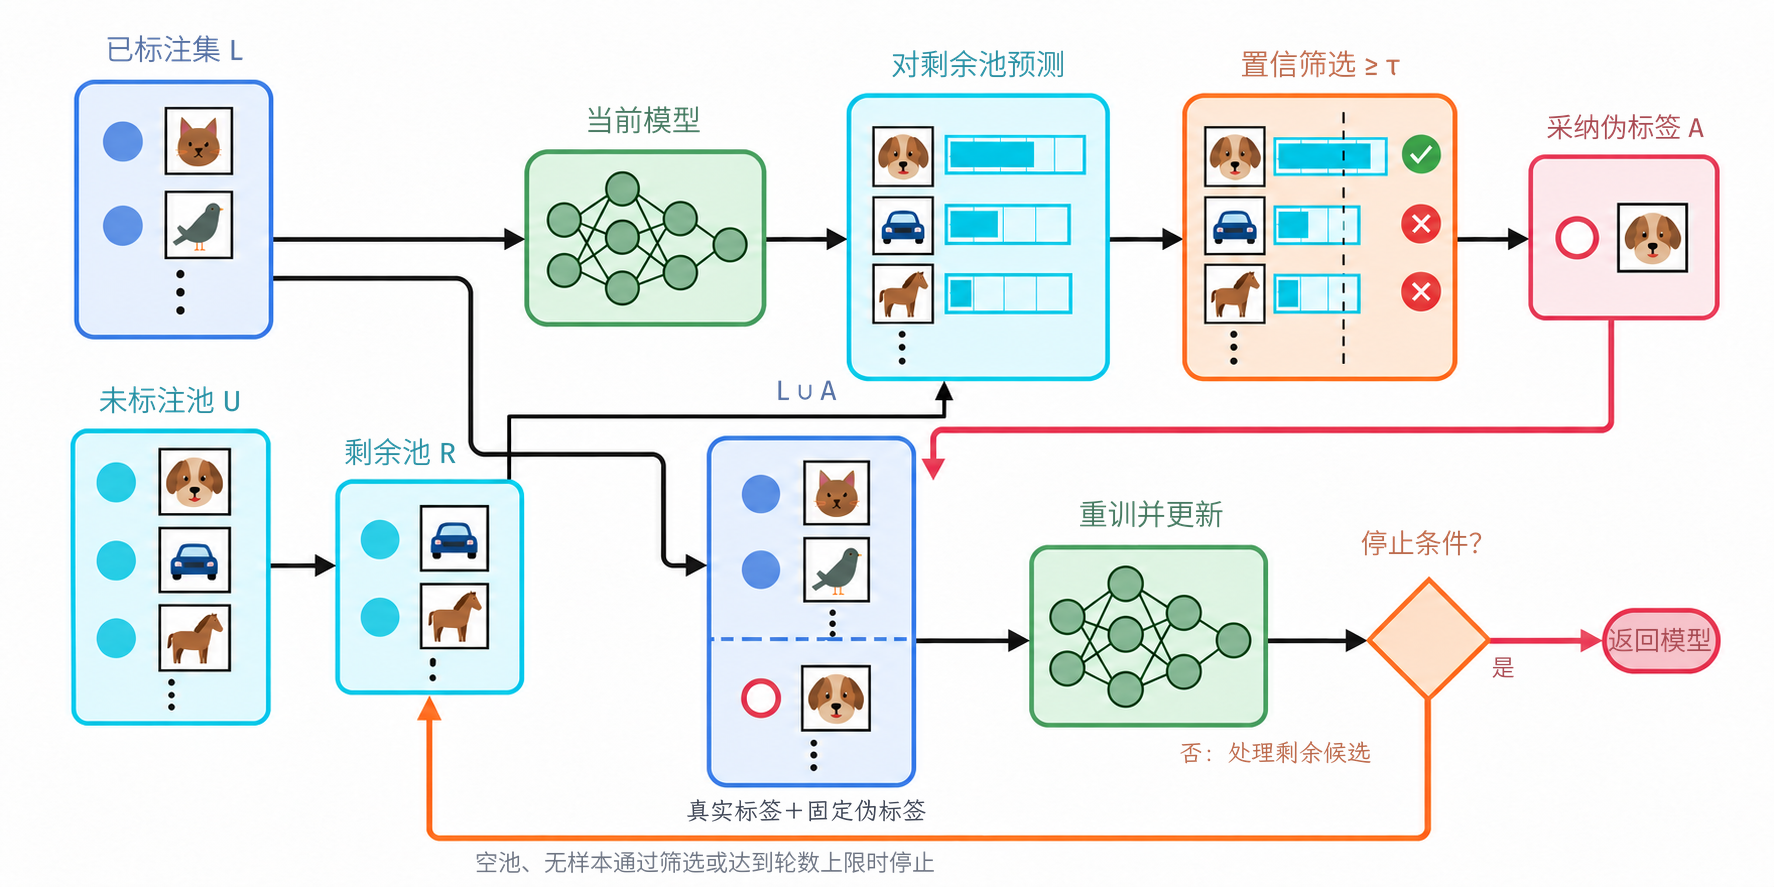
\includegraphics[width=\linewidth]{figures/03-models/01-classic-models/generated/classification-self-training/figure.png}
  \caption{固定阈值、固定已采纳伪标签的自训练流程，对应算法~\ref{alg:classification-self-training}。真实标签保持不变，已采纳的伪标签始终是模型预测。每次采纳后先重训，再用更新后的模型处理剩余候选；空池、无样本通过筛选或达到轮数上限时停止。这个模型反馈回路也可能产生确认偏差：错误预测被当作后续监督，使模型进一步强化原有误判。}
  \label{fig:classification-self-training}
\end{figure*}

阈值并非唯一的筛选手段。每轮可以只采纳通过阈值的前若干个样本，以控制一次错误扩充的影响；也可以按类别限制数量，避免某个易预测类别占据全部新增监督。这些策略改变的是$B^{(t)}$的构造，不改变先保存标签、再扩充集合、随后重训的顺序。类别配额应参考真实任务中的类别比例，不能为了数量整齐就把不平衡任务强行改成均衡任务。

\subsubsection{理论分析}
\label{sec:classification-self-training-analysis}

\paragraph{收敛性分析}
这个基本版本何时停止，可以直接从集合变化判断。每次成功扩充至少从$R$移走一个样本，且样本不会移回，因此成功扩充最多发生$\min\{T,|U|\}$次；若没有样本通过筛选，循环会更早结束。只要每次基分类器训练能够返回，外层循环就会有限终止。这不是对统计最优性的证明，也不代表一列参数收敛到某个固定目标的全局极小值，因为训练集及其监督信号一直在变化。

自训练与\term{熵最小化}（entropy minimization）有共同的倾向：都可能让未标注样本上的预测变得更确定。熵最小化直接惩罚模型预测分布的条件熵，推动概率集中到少数类别。Grandvalet与Bengio讨论了这一准则及其与自训练的联系，但这种联系依赖具体的概率模型和优化设定，不能把所有硬伪标签流程都视为同一个优化问题\scite{grandvalet2004entropy}

对一个未标注输入$\bm{x}$，Shannon熵与硬伪标签交叉熵分别涉及
\begin{equation}
  \label{eq:classification-pseudolabel-entropy}
  \begin{aligned}
    H_{\bm{\theta}}(\bm{x})
      &=-\sum_{c=1}^{C}p_{\bm{\theta}}(c\mid\bm{x})
        \log p_{\bm{\theta}}(c\mid\bm{x}),\\
    \min_{\widetilde y\in\{1,\dots,C\}}
      \{-\log p_{\bm{\theta}}(\widetilde y\mid\bm{x})\}
      &=-\log\max_c p_{\bm{\theta}}(c\mid\bm{x}).
  \end{aligned}
\end{equation}
前者对所有类别求加权和，后者只取概率最大的一个类别，两者数值和梯度一般不同。例如，预测为$(0.8,0.2)$时，以自然对数计算的熵约为$0.500$，最小硬标签交叉熵约为$0.223$。实际自训练还会筛选样本并冻结历史伪标签，因此下一轮甚至不一定仍以当前最大概率类别为目标。

\paragraph{泛化分析}
在平滑性与模型容量约束合适时，提升同一聚集区域内的预测确定性，可能促使决策边界远离该区域；但仅在单个输入上降低熵，并不自动约束附近输入的分类。更关键的是，熵只衡量确定程度，不衡量答案是否正确。若初始分类器错误地把一批同主题文档判成另一类，采纳这些预测后再训练，模型可能对原错误更加确信。这种把自身误判重新当作证据的现象称为\term{确认偏差}（confirmation bias）。Arazo等在深度图像分类实验中观察到，朴素伪标签训练会拟合错误伪标签，并比较了缓解这一现象的正则化方法\scite{arazo2020confirmation}这项证据支持错误可能被反馈回路强化，不构成所有自训练流程必然恶化的普遍定理。

伪标签错误怎样影响真实风险，可以在固定一轮模型后直接推导。令$h$为这一轮产生伪标签的分类器，$\bm{X}_\tau\subseteq\mathbb{R}^{d}$为通过其置信度阈值的输入区域。对目标分布$\mathcal{P}$，用$R_{\mathcal{P}}(f)=\mathbb{P}_{\mathcal{P}}(f(\bm{x})\ne y)$表示任意候选分类器$f$的新样本风险。设$\pi=\mathbb{P}_{\mathcal{P}}(\bm{x}\in\bm{X}_\tau)>0$，在筛选区域内分别考察伪标签自身的错误率，以及$f$与伪标签不一致的概率：
\begin{equation}
  \label{eq:classification-self-training-conditional-risks}
  \begin{aligned}
    e_\tau
      &=\mathbb{P}_{\mathcal{P}}
        \bigl(h(\bm{x})\ne y\mid\bm{x}\in\bm{X}_\tau\bigr),\\
    \widetilde R_\tau(f)
      &=\mathbb{P}_{\mathcal{P}}
        \bigl(f(\bm{x})\ne h(\bm{x})\mid\bm{x}\in\bm{X}_\tau\bigr).
  \end{aligned}
\end{equation}
若$f$预测错误，它要么与$h$不一致，要么沿用了$h$的错误，因此
\begin{equation}
  \label{eq:classification-self-training-error-events}
  \{f(\bm{x})\ne y\}
    \subseteq
    \{f(\bm{x})\ne h(\bm{x})\}
    \cup\{h(\bm{x})\ne y\},
\end{equation}
在$\bm{X}_\tau$内应用并集界，再把区域内外的风险相加，得到
\begin{equation}
  \label{eq:classification-self-training-risk}
  \begin{aligned}
    R_{\mathcal{P}}(f)
      \leq{}&\pi\bigl(\widetilde R_\tau(f)+e_\tau\bigr)\\
      &+\mathbb{P}_{\mathcal{P}}
        \bigl(f(\bm{x})\ne y,\ \bm{x}\notin\bm{X}_\tau\bigr).
  \end{aligned}
\end{equation}
因此，即使$f$完全拟合了该区域的伪标签，也不能据此消除$e_\tau$，更没有控制区域外的错误。这个界描述固定一轮模型及其筛选区域的总体风险关系，不是多轮自训练的风险递减定理；$\widetilde R_\tau(f)$也不是有限伪标签集上的训练误差。采纳事件依赖模型，历史伪标签又由不同轮次产生，不能把$|L|+|A|$直接当成独立真实标签的样本数来套用监督泛化界。

较高阈值能够减少采纳数量，却不能消除系统性高置信度错误。控制伪标签权重与单轮规模、检验不同类别的接受率，以及用保留的真实标签验证集比较扩充前后的性能，分别约束影响强度、类别偏置与实际效果。验证样本不能同时作为被模型反复吸收的伪标签训练样本，否则对自训练收益的估计会失去独立性。若未标注池混入未知类别，或标注数据只覆盖少数容易区域，还需要检查这些不匹配，而不能只调低阈值以追求更多伪标签。

\subsubsection{小结}
\label{sec:classification-self-training-summary}

自训练把已有分类器的部分预测转化为新增监督，适合在保留原有训练和预测接口的情况下探索无标签数据的价值。它的额外成本包括对剩余池反复预测，以及在不断扩大的训练集上重新拟合；基分类器训练昂贵时，这些成本并不小。最终模型仍按原分类器的方式预测新样本，无须保留一个独立的传播图。

是否采用自训练，主要取决于初始预测能否筛出足够可靠且有代表性的样本。标签极少时，恰恰可能无法满足这一条件，所以它不是所有冷启动任务的默认答案；反过来，具备持续验证和错误处理机制时，也没有理由把它限定为只能短期使用。人工复核可以改善部分伪标签的质量，但是否需要、复核哪些样本，应由误判代价与可用预算决定，不能把这一环节当作普遍充分的安全保证。

\subsection{Label Propagation}
\label{sec:classification-label-propagation}

自训练通过基分类器决定哪些预测值得采纳；如果可信的信息主要来自样本之间的邻近关系，也可以直接在这些关系上传递标签。\term{标签传播}（label propagation）把样本表示为图的节点，让已有标签沿相似边影响尚无标签的节点。Zhu与Ghahramani在2002年的技术报告中给出了保持已知标签不变的传播方法\scite{zhu2002labelpropagation}与只在已标注样本中寻找近邻相比，未标注点也参与形成传播路径，使标签能够沿弯曲的高密度区域传递；每轮恢复已知标签，则让它们持续提供监督，不会因反复平均而失去原有的类别信息。

本节采用与调和函数解释一致的随机游走记号，明确区分这种硬边界传播与后面介绍的软约束版本。

\subsubsection{模型结构}
\label{sec:classification-label-propagation-structure}

图模型把“哪些输入相似”转化成可计算的边权。令$\mathcal{G}=(V,E,\bm{W})$，其中$V=L\cup U$，$\bm{W}\in\mathbb{R}^{n\times n}$为非负对称权重矩阵，$\bm{W}_{i,j}=\bm{W}_{j,i}\geq0$，且取$\bm{W}_{i,i}=0$。例如，可以先选出近邻边，再在相连节点上使用RBF相似度
\begin{equation}
  \label{eq:classification-label-propagation-weights}
  \bm{W}_{i,j}=
  \begin{cases}
    \exp\bigl(-\gamma\lVert\bm{x}_i-\bm{x}_j\rVert_2^2\bigr),
      & \{i,j\}\in E,\\
    0, & \text{其他情形},
  \end{cases}
\end{equation}
其中$\gamma>0$控制相似度衰减。用$k$近邻关系构图时，单向近邻关系需要经过并集或互近邻等明确规则转成无向边，才能满足对称性。完全图保留所有样本对，稀疏图只保留选中的关系；两者不仅存储成本不同，也可能给出不同的分类结果。

每个节点的加权度记为$\delta_i=\sum_j\bm{W}_{i,j}$，度矩阵满足$\bm{D}_{i,i}=\delta_i$。在所有参与传播的节点度数为正时，定义
\begin{equation}
  \label{eq:classification-label-propagation-transition}
  \bm{P}=\bm{D}^{-1}\bm{W},
  \qquad
  \bm{P}_{i,j}=\frac{\bm{W}_{i,j}}{\delta_i}.
\end{equation}
矩阵$\bm{P}$每行的和为1，表示从一个节点沿边随机走向邻居的转移概率。传播时用这一行权重对邻居的标签信息求平均；权重大，邻居的影响也大。

为了同时处理$C$个类别，令$\bm{F}\in\mathbb{R}^{n\times C}$保存节点得分，$\bm{f}_i=(\bm{F}_{i,1},\dots,\bm{F}_{i,C})^\top$为节点$i$的得分向量。构造同形状的$\bm{Y}$：若$i\in L$，则$\bm{Y}_{i,c}=\mathbb{1}\{y_i=c\}$；若$i\in U$，则整行置零。有标签节点在每轮更新后都恢复到这份独热编码，这种固定边界的操作称为\term{硬钳制}（hard clamping），也就是不允许传播改变已经给定的标签。

构图时必须检查标签信息能否到达每个待预测节点。零度无标签节点没有邻居，无法定义式~\eqref{eq:classification-label-propagation-transition}~中的转移概率；一个连通分量若完全没有标签，即使每个节点度数都大于零，也无法确定任何类别。可以补充真实标签、依据可靠关系重新构图，或对这些节点明确拒绝预测。孤立的有标签节点保留原标签即可，不必参与传播。仅增加一个微小度数或自环，只解决部分数值形式问题，并没有给缺少监督的分量提供类别信息。

\subsubsection{参数学习}
\label{sec:classification-label-propagation-learning}

标签传播没有固定维数的分类器参数要拟合，但需要求出全部无标签节点的得分。下面假设零度节点已经处理，每个含无标签节点的连通分量至少含一个有标签节点。把$\bm{F}$按$L$与$U$分成行块$\bm{F}_L=\bm{F}_{L,:}$、$\bm{F}_U=\bm{F}_{U,:}$，并对$\bm{P}$作对应分块。硬钳制意味着$\bm{F}_L^{(t)}=\bm{Y}_L$始终不变，因而只需迭代
\begin{equation}
  \label{eq:classification-label-propagation-iteration}
  \bm{F}_U^{(t+1)}
    =\bm{P}_{U,U}\bm{F}_U^{(t)}
     +\bm{P}_{U,L}\bm{Y}_L.
\end{equation}
右侧第一项传递尚无标签节点之间的当前信息，第二项持续注入真实标签。通常取$\bm{F}_U^{(0)}=\bm{0}$。这个硬钳制方案不需要再引入传播系数$\alpha$，也不在有标签节点上附加一个有限权重的软拟合项。

若迭代达到固定点，移项便得到线性系统与形式上的闭式解
\begin{equation}
  \label{eq:classification-label-propagation-solution}
  \begin{aligned}
    (\bm{I}-\bm{P}_{U,U})\bm{F}_U^\ast
      &=\bm{P}_{U,L}\bm{Y}_L,\\
    \bm{F}_U^\ast
      &=(\bm{I}-\bm{P}_{U,U})^{-1}
        \bm{P}_{U,L}\bm{Y}_L.
  \end{aligned}
\end{equation}
这里$\bm{I}$为$|U|\times|U|$单位矩阵。下一小节将证明，在上述图条件下逆矩阵存在，且任意初始化的迭代都收敛到同一个解。计算时通常直接求解线性系统，避免显式构造逆矩阵。Zhu、Ghahramani与Lafferty给出了这一解的调和函数、图能量和随机游走解释\scite{zhu2003}

图\ref{fig:classification-label-propagation}给出一个可逐项核算的教学构造，并非实测数据。五个节点依次相连，每条无向边的权重为1；端点1固定属于类1，端点5固定属于类2，节点2、3、4没有标签。令$p_i=\bm{F}_{i,1}^\ast$，由于每个内点恰有两个等权邻居，式~\eqref{eq:classification-label-propagation-iteration}~在固定点处变为
\begin{equation}
  \label{eq:classification-label-propagation-path}
  \begin{aligned}
    p_i&=\frac{p_{i-1}+p_{i+1}}{2},
      &&i=2,3,4,\\
    p_1&=1,\qquad p_5=0.
  \end{aligned}
\end{equation}
内点方程等价于$p_{i+1}-p_i=p_i-p_{i-1}$，所以相邻节点的得分差必须相等。两端总共下降1，分到四条边上，每步下降$1/4$，得到
\[
  (p_1,p_2,p_3,p_4,p_5)
    =(1,0.75,0.5,0.25,0).
\]
类2的得分满足相反的端点条件，故$\bm{f}_i^\ast=(p_i,1-p_i)^\top$。节点2偏向类1，节点4偏向类2；节点3的两类得分相同，按本节“并列时取最小类别编号”的约定判为类1。这个离散判定只是处理并列的规则，不能被解释为节点3存在支持类1的额外证据。

\begin{figure}[htbp]
  \centering
  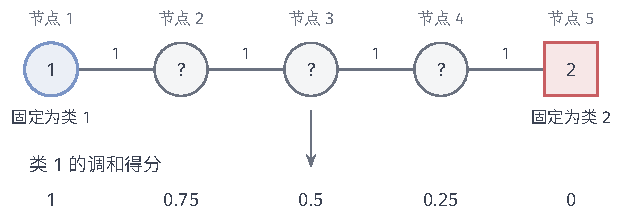
\includegraphics[width=\linewidth]{figures/03-models/01-classic-models/tikz/classification-label-propagation/figure.pdf}
  \caption{五节点等权无向路径上的硬钳制标签传播。每条边权为1，左端圆形节点固定为类1，右端方形节点固定为类2，问号表示未知标签。下方列出精确调和解的类1得分，类2得分为其补数；内点得分等于两侧邻居的平均。中间节点两类并列，按最小类别编号规则判为类1。这是教学构造，不是实测结果。}
  \label{fig:classification-label-propagation}
\end{figure}

迭代实现还需要把停止条件与返回值对应起来。算法\ref{alg:classification-label-propagation}使用相邻两轮之差作为数值停止判据，其中$\lVert\cdot\rVert_{\mathrm{F}}$为Frobenius范数，$\varepsilon>0$为容限，$T\geq1$为最大迭代次数。若达到上限时仍未满足容限，返回的状态必须保留这一信息，不能把“运行结束”报告为“已经收敛”。

\begin{algorithm}[硬钳制标签传播]
  \label{alg:classification-label-propagation}
  \begin{algorithmic}[1]
    \Require 权重$\bm{W}$、索引$L,U$、标签矩阵$\bm{Y}$
    \Require 容限$\varepsilon>0$、最大迭代次数$T\geq1$
    \Ensure 得分$\bm{F}$、预测$\widehat{\bm{y}}_U$及停止状态
    \If{$U=\varnothing$}
      \State \Return $\bm{Y}$、空预测、已完成
    \EndIf
    \State 检查$\bm{W}$非负、对称，参与传播的节点度数为正
    \State 检查每个含$U$节点的连通分量至少有一个$L$节点
    \If{任何检查失败}
      \State \Return 拒绝结果，要求补标签或修正传播图
    \EndIf
    \State 构造$\bm{P}=\bm{D}^{-1}\bm{W}$
    \State $\bm{F}_L\gets\bm{Y}_L$，$\bm{F}_U\gets\bm{0}$
    \State $\mathrm{converged}\gets\mathrm{false}$
    \For{$t=1,\dots,T$}
      \State $\bm{G}\gets\bm{P}_{U,U}\bm{F}_U+\bm{P}_{U,L}\bm{Y}_L$
      \State $\Delta\gets\lVert\bm{G}-\bm{F}_U\rVert_{\mathrm{F}}$
      \State $\bm{F}_U\gets\bm{G}$
      \If{$\Delta\leq\varepsilon(1+\lVert\bm{F}_U\rVert_{\mathrm{F}})$}
        \State $\mathrm{converged}\gets\mathrm{true}$
        \State \textbf{break}
      \EndIf
    \EndFor
    \State $\widehat y_j\gets\argmax_c\bm{F}_{j,c}$，$j\in U$；并列取最小$c$
    \State \Return $\bm{F},\widehat{\bm{y}}_U,\mathrm{converged}$
  \end{algorithmic}
\end{algorithm}

算法先把$\bm{G}$保存成最新的$\bm{F}_U$，再判断是否退出，因此即使本轮达到容限，也会返回新得分而不是上一轮的值。相邻迭代差小是一种可操作的停止指标，不直接给出距离精确解的统一误差界；当传播很慢时，还需结合线性系统残差与条件数判断数值精度。最终类别由得分比较决定，接近平局的节点尤其需要保留得分与未收敛状态。

\subsubsection{理论分析}
\label{sec:classification-label-propagation-analysis}

\paragraph{收敛性分析}
硬钳制传播能够收敛，关键不是“每个节点都直接连着标签”，而是未标注节点经过若干步能够到达有标签节点。$\bm{P}_{U,U}$每一行的和至多为1，其中某些行可以恰好等于1，因为对应节点暂时只有无标签邻居。要证明收缩，需要考察多步传播后仍然留在$U$中的总权重。

\begin{theorem}[硬钳制传播的唯一解]
  \label{thm:classification-label-propagation-convergence}
  设图有限、边权非负且对称，所有参与传播的节点度数为正，$U$非空，且每个含无标签节点的连通分量至少含一个有标签节点。则$\rho(\bm{P}_{U,U})<1$，其中$\rho$表示谱半径。式~\eqref{eq:classification-label-propagation-iteration}~从任意初始得分出发，都收敛到式~\eqref{eq:classification-label-propagation-solution}~中的唯一固定点。
\end{theorem}

\begin{proof}
  从每个$j\in U$出发，选择一条到达$L$的正权路径，并在首次到达$L$时停止。有限图中这些路径长度有一个共同上界$m$，沿各路径行走的概率均为正，其最小值记为$\epsilon>0$。于是，无论从哪个无标签节点出发，在$m$步以内命中$L$的概率都至少为$\epsilon$。这说明
  \[
    \lVert\bm{P}_{U,U}^{m}\rVert_\infty\leq1-\epsilon,
    \qquad
    \rho(\bm{P}_{U,U})^m\leq1-\epsilon<1.
  \]
  因而$\bm{P}_{U,U}^t$趋于零，Neumann级数收敛，且
  \[
    (\bm{I}-\bm{P}_{U,U})^{-1}
      =\sum_{t=0}^{\infty}\bm{P}_{U,U}^{t}.
  \]
  迭代展开为
  \[
    \bm{F}_U^{(t)}
      =\bm{P}_{U,U}^{t}\bm{F}_U^{(0)}
       +\sum_{s=0}^{t-1}
         \bm{P}_{U,U}^{s}\bm{P}_{U,L}\bm{Y}_L.
  \]
  第一项消失，第二项趋于所述固定点。逆矩阵存在，也排除了其他固定点。
\end{proof}

还可以从最优化的角度解释同一个解。相邻节点的得分差越大，图上的不平滑程度越高。令$\bm{L}_{\mathrm{g}}=\bm{D}-\bm{W}$为\term{图拉普拉斯矩阵}（graph Laplacian），它把这种局部差异汇总成二次型。固定真实标签边界后，求解的\term{狄利克雷能量}（Dirichlet energy）最小化问题为
\begin{equation}
  \label{eq:classification-label-propagation-energy}
  \begin{aligned}
    \min_{\bm{F}:\,\bm{F}_L=\bm{Y}_L}\quad
    \mathcal{E}(\bm{F})
      &=\frac12\sum_{i,j=1}^{n}
        \bm{W}_{i,j}\lVert\bm{f}_i-\bm{f}_j\rVert_2^2\\
      &=\operatorname{tr}
        (\bm{F}^{\top}\bm{L}_{\mathrm{g}}\bm{F}).
  \end{aligned}
\end{equation}
第\ref{sec:clustering-spectral}节的谱聚类与第\ref{sec:dim-le}节的拉普拉斯特征映射复用图拉普拉斯和谱工具，但输出分别是离散簇分配与连续低维坐标；这里的标签传播则在已知类别语义下求类别得分。共享图结构不意味着三个任务使用相同的输出约束。

有标签节点在这里是固定边界，不是可以通过支付有限罚项而改变的变量。对未知行块求导并令其为零，得到
\begin{equation}
  \label{eq:classification-label-propagation-dirichlet}
  \begin{aligned}
    (\bm{L}_{\mathrm{g}})_{U,U}\bm{F}_U
      &=-(\bm{L}_{\mathrm{g}})_{U,L}\bm{Y}_L\\
      &=\bm{W}_{U,L}\bm{Y}_L.
  \end{aligned}
\end{equation}
因为$(\bm{L}_{\mathrm{g}})_{U,U}=\bm{D}_{U,U}-\bm{W}_{U,U}$，左乘$\bm{D}_{U,U}^{-1}$就回到式~\eqref{eq:classification-label-propagation-solution}~的线性系统。

这个驻点也是唯一最小值，而不只是一个形式上的导数解。取任意无标签节点上的非零向量$\bm{z}$，把它扩展成在$L$上为零的全图向量$\widetilde{\bm{z}}$，则
\[
  \bm{z}^{\top}(\bm{L}_{\mathrm{g}})_{U,U}\bm{z}
    =\frac12\sum_{i,j}\bm{W}_{i,j}
      (\widetilde z_i-\widetilde z_j)^2.
\]
右侧若为零，向量在每个正权连通分量上就必须为常数。每个涉及$U$的分量又含一个值为零的标签边界，因此这些常数只能全部为零，与$\bm{z}\ne\bm{0}$矛盾。故未标记主子块正定，能量对$\bm{F}_U$严格凸。这同时解释了为什么完全无标签的分量会破坏唯一性：在这种分量上，任意常值向量都不增加图能量。

得分的概率含义也需要依赖这些条件。从一个无标签节点按$\bm{P}$行走，并在首次碰到有标签节点时停止，$\bm{F}_{j,c}^\ast$等于首次命中的标签属于类$c$的概率。由于最终命中$L$的概率为1，精确解各行非负且行和为1。若从零初始化，有限轮得分只累积了相应步数内的命中概率，行和可能还小于1；一般不能把尚未收敛的得分直接当成归一化概率。即便在极限处，这也是给定图上的命中概率，不自动等于真实任务中校准的类别后验。

\paragraph{泛化分析}
优化的唯一性没有检验图是否表达了正确的类别关系。\term{平滑假设}（smoothness assumption）在这里意味着强相似边连接的节点应具有相近标签得分；若文档按写作风格聚集却按主题分类，这个假设就可能失效。跨类强边会把错误信息传到邻域，错误的标签边界还会被硬钳制持续保留。高维距离失真时，特征标准化、降维或度量学习可以改善构图的候选表示，但这些处理同样需要验证，不能由线性系统收敛来证明其合理性。

这里还要区分两种评价对象。对非空$U$，在训练之外取得真实标签后，可以计算
\begin{equation}
  \label{eq:classification-label-propagation-pool-risk}
  \widehat R_U
    =\frac{1}{|U|}\sum_{j\in U}
      \mathbb{1}\{\argmax_c\bm{F}_{j,c}^\ast\ne y_j\}.
\end{equation}
其中并列得分仍按最小类别编号处理，$y_j$只用于评价。这个误差针对已经参与构图的输入，不是对未来独立样本风险的直接估计。要讨论新样本，还必须定义归纳扩展$h_{\mathcal{G}}(\bm{x})$，即规定新输入如何连接到图、怎样由图上得分产生预测，以及是否重新求解；这时才有相应的风险$R_{\mathcal{P}}(h_{\mathcal{G}})=\mathbb{P}_{\mathcal{P}}(h_{\mathcal{G}}(\bm{x})\ne y)$。

前述定理没有对$R_{\mathcal{P}}(h_{\mathcal{G}})$给出上界：它既未规定这种扩展，也未假设新样本与图上标签之间的统计关系。若要建立随样本数变化的风险保证，还需把构图规则、标签覆盖和类别平滑性等条件与目标分布联系起来。对一个给定图求出唯一解，只解决了得分怎样确定，不能替代这些条件。

\subsubsection{小结}
\label{sec:classification-label-propagation-summary}

标签传播适合相似关系本身可信的任务，例如有可靠连接语义的节点分类，或用局部外观关系传播图像块标签。其基本输出是当前图上各节点的得分，适合面向这批输入作出预测；若任务持续接收新输入，前述归纳扩展也应纳入模型设计和评价。

计算成本取决于图的稀疏性与求解精度，而不是一个固定的节点数分界。记$\operatorname{nnz}(\bm{W})$为非零权重数，稀疏图一次传播的主要乘法成本为$O(\operatorname{nnz}(\bm{W})C)$，存储主要为$O(\operatorname{nnz}(\bm{W})+nC)$；总时间还要乘以迭代次数，并另计构图成本。完全图的存储为$O(n^2)$，直接计算所有欧氏距离通常需$O(n^2d)$。即使图很稀疏，连接标签区域的边过弱，也会使$\rho(\bm{P}_{U,U})$接近1，导致传播缓慢。

可以利用稀疏线性求解器，或在合适的相似度矩阵上使用\term{Nyström近似}（Nyström approximation），即选取少量代表列来构造低秩近似，减少矩阵运算。但近似相似度不一定保留原图的非负边权、连通关系与硬边界解；采用近似后应重新检查这些条件和求解误差。图上的唯一解、数值上的近似精度以及分类准确率，是三个需要分别评价的问题。

\subsection{TSVM}
\label{sec:classification-tsvm}

图传播直接平滑节点得分；若希望保留SVM的分类函数，则可以让无标签样本参与选择大间隔边界。\term{直推支持向量机}（transductive support vector machine, TSVM）同时选择分类器与当前未标注样本的标签，使两类样本共同约束间隔。Joachims在1999年的文本分类研究中给出了有代表性的目标与实用求解算法。其相关性反馈任务说明了这一选择的背景：用户只标注少量检索结果是否相关，其余待分类文档却已经构成一个给定的文档库。于是，这些文档不必等到训练结束后才交给分类器，而可以在训练时通过自身的位置参与确定间隔边界\scite{joachims1999transductive}

这里的\term{直推学习}（transductive learning，也称转导学习）指利用当前已给定的待预测输入，直接推断这批输入的标签；它与面向未来新输入评价预测规则的归纳设定有所区别。TSVM仍会得到一个SVM分类函数，所以从计算上也能处理新样本。区别在于哪些输入参与了训练，以及理论或实验评价针对哪批预测，而不是算法是否能够写出一个函数。

\subsubsection{模型结构}
\label{sec:classification-tsvm-structure}

本小节使用二分类标签$\{-1,+1\}$。令$g(\bm{x})=\bm{w}^{\top}\phi(\bm{x})+b$为决策分数，$\phi$为选定的特征映射；线性SVM取$\phi(\bm{x})=\bm{x}$。标准软间隔SVM只要求已标注样本尽量满足$y_i g(\bm{x}_i)\geq1$。TSVM还为每个$j\in U$引入一个待选择的离散标签$y_j^{\mathrm{u}}$，并为相应间隔约束配置松弛变量$\xi_j^{\mathrm{u}}$。其目标可写为
\begin{equation}
  \label{eq:classification-tsvm-objective}
  \begin{aligned}
    \min_{\bm{w},b,\bm{y}^{\mathrm{u}},\bm{\xi}}\quad
    \mathcal{J}
      ={}&\frac12\lVert\bm{w}\rVert_2^2
         +\lambda_{\mathrm{s}}\sum_{i\in L}\xi_i\\
       &+\lambda_{\mathrm{u}}\sum_{j\in U}\xi_j^{\mathrm{u}},
  \end{aligned}
\end{equation}
其中$\bm{y}^{\mathrm{u}}$收集无标签节点的离散标签，$\bm{\xi}$收集两类松弛变量，$\lambda_{\mathrm{s}}>0$与$\lambda_{\mathrm{u}}\geq0$分别控制有标签项和无标签项的惩罚。约束为
\begin{equation}
  \label{eq:classification-tsvm-constraints}
  \begin{aligned}
    y_i g(\bm{x}_i)&\geq1-\xi_i,
      &\xi_i&\geq0,\quad i\in L,\\
    y_j^{\mathrm{u}}g(\bm{x}_j)&\geq1-\xi_j^{\mathrm{u}},
      &\xi_j^{\mathrm{u}}&\geq0,\quad j\in U,\\
    y_j^{\mathrm{u}}&\in\{-1,+1\},
      &&j\in U,\\
    \sum_{j\in U}\frac{1+y_j^{\mathrm{u}}}{2}&=r.
  \end{aligned}
\end{equation}
最后一行固定无标签样本中的正类标签数量$r$。本节讨论$|U|\geq2$且$1\leq r\leq|U|-1$的非退化情形；$\lambda_{\mathrm{u}}=0$或$U$为空时，分类器训练回到纯监督SVM。

类别数量约束来自一个实际困难：无标签样本本身不能说明哪一侧应有多少样本。若只要求间隔大，模型可能把几乎全部未标注样本放到同一类，从而得到不符合任务的划分。\term{类别平衡约束}（class-balance constraint）把对类别组成的外部知识加入优化，它不要求两类数量相等，而是固定或限制可接受的比例。可以根据可信先验选择$r$，也可以规定$r_{\min}\leq\sum_j(1+y_j^{\mathrm{u}})/2\leq r_{\max}$。由少量已标注样本估计比例时，需要考虑抽样偏差；错误的比例约束同样会损害结果。

约束的是待优化标签的数量，不是带松弛的分类器最终必须恰好预测$r$个正类。个别样本仍可能被分错或落在间隔内。明确这一区别，才能理解为什么固定比例的标签交换是可行操作，却不保证每次训练后的正预测比例完全不变。

无标签项怎样影响边界，可以暂时去掉数量约束来观察。对给定分数$s$，若允许独立选择二分类标签，最小的无标签合页损失为
\begin{equation}
  \label{eq:classification-tsvm-unlabeled-hinge}
  \min_{y\in\{-1,+1\}}[1-ys]_+=[1-|s|]_+,
\end{equation}
其中$[a]_+=\max\{a,0\}$。这项损失惩罚分数靠近零的无标签样本，却不预先规定它们应落在哪一侧。在合适的表示下，若大量输入集中在少数区域，让边界避开这些区域就能减少此项损失。这是\term{低密度分离假设}（low-density separation assumption）的作用：类别分界应经过输入较少的区域，而不是切开高密度的同类区域。恢复类别数量约束后，各个标签选择相互耦合，不能再逐样本独立最小化。

\subsubsection{参数学习}
\label{sec:classification-tsvm-learning}

固定$\bm{y}^{\mathrm{u}}$以后，式~\eqref{eq:classification-tsvm-objective}~就是具有不同样本惩罚的软间隔SVM，可以沿用相应凸优化求解器。困难在于标签本身还要选择：固定正类数$r$时有$\binom{|U|}{r}$种标签配置，通常无法逐一求解比较。实用算法从监督SVM出发，交替改善标签与分类器，并逐步提高$\lambda_{\mathrm{u}}$，使无标签数据的影响从弱变强。

初始化也要满足数量约束。先在$L$上训练监督SVM，按它对$U$的决策分数排序，把分数最高的$r$个样本暂定为正类，其余为负类；分数并列时按样本索引排序。直接使用监督分类器的正负预测，不一定能得到规定的正类数，因此不能替代这一步。

在固定$\lambda_{\mathrm{u}}>0$的一轮内，可以交换一个当前正类样本$a$与负类样本$b$的标签。这样正类总数不变，只需判断交换是否有利。记$\ell_{\mathrm{h}}(s)=[1-s]_+$，在当前分类器分数不变时，交换带来的无标签损失变化为
\begin{equation}
  \label{eq:classification-tsvm-swap}
  \begin{aligned}
    \Delta_{a,b}
      ={}&\ell_{\mathrm{h}}\bigl(-g(\bm{x}_a)\bigr)
          +\ell_{\mathrm{h}}\bigl(g(\bm{x}_b)\bigr)\\
       &-\ell_{\mathrm{h}}\bigl(g(\bm{x}_a)\bigr)
          -\ell_{\mathrm{h}}\bigl(-g(\bm{x}_b)\bigr).
  \end{aligned}
\end{equation}
若$\Delta_{a,b}<0$，仅交换标签并相应调整松弛变量，就已经降低了目标中的无标签项；随后重新求解固定标签的SVM，目标值只会进一步降低或保持不变。这个判据给出一类易于检查的下降交换，而不是穷尽所有可能使重训结果改善的标签变化。

算法\ref{alg:classification-tsvm}采用这一下降判据说明求解过程。$\operatorname{FitSVM}(\bm{y}^{\mathrm{u}},\lambda_{\mathrm{u}})$表示在当前固定标签下，用有标签惩罚$\lambda_{\mathrm{s}}$和无标签惩罚$\lambda_{\mathrm{u}}$完整求解SVM。原始实现还可以为未标注正负类使用不同惩罚；这里用统一的$\lambda_{\mathrm{u}}$突出类别平衡、交换与逐步加权的关系。

\begin{algorithm}[固定类别数量的TSVM逐步加权]
  \label{alg:classification-tsvm}
  \begin{algorithmic}[1]
    \Require 含两个类别的训练索引$L$，无标签索引$U$
    \Require $|U|\geq2$，正类数量$1\leq r\leq|U|-1$
    \Require $\lambda_{\mathrm{s}}>0$，目标$\lambda_{\mathrm{u}}^{\mathrm{final}}>0$
    \Require 初值$\lambda_{\mathrm{u}}^{(0)}>0$，倍率$q>1$，容限$\varepsilon\geq0$
    \Ensure 分类器$g$及离散标签$\bm{y}^{\mathrm{u}}$
    \State 在$L$上训练监督SVM，得到$g$
    \State 按$g$的分数将$U$中前$r$个样本标为正，其余标为负
    \State $\lambda_{\mathrm{u}}\gets
      \min\{\lambda_{\mathrm{u}}^{(0)},\lambda_{\mathrm{u}}^{\mathrm{final}}\}$
    \While{尚未在目标惩罚值下完成训练}
      \State $g\gets\operatorname{FitSVM}(\bm{y}^{\mathrm{u}},\lambda_{\mathrm{u}})$
      \While{存在正负标签对$(a,b)$使$\Delta_{a,b}<-\varepsilon$}
        \State 交换$y_a^{\mathrm{u}}$与$y_b^{\mathrm{u}}$
        \State $g\gets\operatorname{FitSVM}(\bm{y}^{\mathrm{u}},\lambda_{\mathrm{u}})$
      \EndWhile
      \If{$\lambda_{\mathrm{u}}=\lambda_{\mathrm{u}}^{\mathrm{final}}$}
        \State \textbf{break}
      \EndIf
      \State $\lambda_{\mathrm{u}}\gets
        \min\{q\lambda_{\mathrm{u}},\lambda_{\mathrm{u}}^{\mathrm{final}}\}$
    \EndWhile
    \State \Return $g,\bm{y}^{\mathrm{u}}$
  \end{algorithmic}
\end{algorithm}

逐步增加无标签惩罚常称为\term{退火}（annealing）：先在真实标签主导的目标上取得初始解，再逐渐增加无标签约束的影响。这里的每个阶段都先训练并完成交换搜索，再判断是否已经达到最终惩罚值。即使某次更新刚好把惩罚设为目标值，也仍需进入下一阶段训练，不能在更新数值后直接返回旧模型。若另设总时间或阶段数量上限，应把提前终止作为未完成目标惩罚训练的状态返回。

这一过程使用上一阶段的结果作初始化，可视为一种延续求解策略，但离散标签变化可能使解发生跳变，不保证存在一条光滑的解路径。退火倍率、初始标签和交换搜索方式会改变最终结果，适合通过多个合理初始化与独立验证比较，而不是把逐步加权当作全局最优算法。

\subsubsection{理论分析}
\label{sec:classification-tsvm-analysis}

\paragraph{收敛性分析}
固定标签子问题的凸性，不会使标签与参数联合优化也变凸。式~\eqref{eq:classification-tsvm-unlabeled-hinge}~已经显示出其中的非凸性：在$s=-1$和$s=1$处损失均为零，在中点$s=0$处却为1，不满足凸函数的中点不等式。实际问题又包含离散标签及其数量限制，因而是连续变量与离散变量耦合的非凸优化问题。求解一个固定标签的SVM与搜索标签配置，是两项不同的工作。

在固定惩罚值下，算法的有限终止可以有一个明确但有限的保证。假设每次固定标签的SVM都求到全局最小值，并且只接受式~\eqref{eq:classification-tsvm-swap}~所给出的严格下降交换。令$V(\bm{y}^{\mathrm{u}})$为当前标签配置对应的最优目标值，则一次接受交换后有
\[
  V(\bm{y}_{\mathrm{new}}^{\mathrm{u}})
    \leq V(\bm{y}_{\mathrm{old}}^{\mathrm{u}})
      +\lambda_{\mathrm{u}}\Delta_{a,b}
    <V(\bm{y}_{\mathrm{old}}^{\mathrm{u}}).
\]
可行标签配置有限，因此不能在严格下降过程中反复回到同一配置，内层搜索最终会停止。倍率$q>1$并在目标值处截断，也保证外层惩罚阶段有限。这一结论依赖精确子问题求解与严格下降；使用数值近似时，需要检查重训后的实际目标变化，不能只根据理想化推导接受任意交换。

停止只说明当前搜索规则没有找到可接受的改进。即使任何交换在固定$g$时都不下降，也仍可能存在交换后充分重训才改善的解，或者需要同时改变多个标签才能到达的更好配置。因此，这个停止条件既不保证全局最优，也不保证对所有单对交换重训都已最优。不同$\lambda_{\mathrm{u}}$阶段之间的目标函数也不同，跨阶段的目标值不构成同一目标下的下降序列。

\paragraph{泛化分析}
统计上的风险来自另一组条件。如果两个真实类别在同一高密度区域内严重重叠，正确的分类边界可能就需要穿过该区域。较大的$\lambda_{\mathrm{u}}$却会奖励避开它的边界，导致无标签数据拉低分类性能。错误的类别比例、未标注池中的未知类别，以及只对局部区域可靠的初始监督模型，也可能产生类似损害。优化更充分并不能修复失效的分布假设，有时反而会更彻底地实现一个不适合任务的目标。

因而，TSVM的效果应与同样特征、同样有标签训练集上的监督SVM比较，并用没有参与调参的真实标签评价。允许训练时看到当前待预测输入，是直推实验设定的一部分；它不能被报告成对完全未见输入的同等保证。若最终用途是归纳预测，还需要另外检查新样本上的表现。

一种不依赖TSVM优化过程的检查，是在训练与调参全部完成后，固定最终分类规则$f$，再用$m\geq1$个独立来自目标分布$\mathcal{P}$的真实标注测试样本评价。这些样本的输入也不参与训练、特征拟合或模型选择。记其零一测试误差为$\widehat R_{\mathrm{test}}(f)$；条件于训练所得的$f$，每个测试错误都是均值为$R_{\mathcal{P}}(f)$的独立Bernoulli变量。由
\BookEquationRef{eq:hoeffding-fixed-hypothesis}{第二卷“基础、理论和可信性”的“二分类学习的可学习性”章中的Hoeffding不等式}，
对$0<\delta<1$，至少以$1-\delta$的概率有
\begin{equation}
  \label{eq:classification-semisupervised-test-risk}
  R_{\mathcal{P}}(f)
    \leq\widehat R_{\mathrm{test}}(f)
       +\sqrt{\frac{\log(2/\delta)}{2m}}.
\end{equation}
这个界把独立测试误差联系到新样本风险，也适用于固定后的自训练分类器或已定义归纳扩展的图分类器。它不是半监督方法优于监督基线的保证；界中的$m$只计独立测试样本，不能换成训练时使用的无标签数量。反复查看这批测试结果后再选择模型，会破坏上述固定分类器的前提，需要另作模型选择校正或保留新的独立测试集。

\subsubsection{小结}
\label{sec:classification-tsvm-summary}

TSVM保留了SVM的决策函数，把变化集中在训练目标与离散标签搜索中。预测新输入时仍计算$g(\bm{x})$并取其符号；分数恰为零时，应使用预先约定的并列规则。它适用于大间隔与低密度分离有合理联系、类别组成可约束的任务，而不是只要无标签样本多就值得引入。

训练开销主要来自反复求解带权SVM与搜索标签交换，受到基求解器、核矩阵规模、惩罚阶段和搜索策略共同影响。类别数量约束避免部分退化解，逐步加权改善求解起点的利用方式，但都不能保证准确率超过监督基线。后面的安全半监督方法进一步研究怎样限制可能的损害，其保证仍有特定前提，不能作为TSVM在任意数据上有效的替代条件。

\subsection{模型对比与总结}
\label{sec:classification-semisupervised-comparison}

本小节先比较Self-Training、Label Propagation与TSVM，再补充生成式EM、多视图训练、软传播、流形正则化和安全选择等代表性扩展。三种基本方法使用的是同一类额外资源，即没有可用标签的输入，但它们从中提取的信息不同。自训练借助现有模型选择补充监督，标签传播把相似关系转成得分平滑约束，TSVM让输入分布参与间隔边界的选择。表\ref{tab:classification-semisupervised-comparison}还加入生成式EM入口；这些机制可以共享假设，也可以组合，不能视为彼此互不重叠的分类。

\begin{table}[htbp]
  \centering
  \small
  \begin{tabularx}{\linewidth}{@{}>{\RaggedRight\arraybackslash}p{25mm}>{\RaggedRight\arraybackslash}X>{\RaggedRight\arraybackslash}X@{}}
    \toprule
    方法 & 无标签数据怎样参与 & 关键条件与代价 \\
    \midrule
    Self-Training & 筛选预测作伪标签，反复训练原分类器 & 采纳的预测应可靠；需反复预测与重训，警惕确认偏差。 \\
    Label Propagation & 在固定标签边界下求图上调和得分 & 图应反映类别关系，且无标签分量能到达标签；成本依赖边数与求解精度。 \\
    TSVM & 联合选择离散标签与大间隔分类器 & 低密度分离及类别数量约束应合理；需要非凸标签搜索与多次SVM训练。 \\
    生成式EM & 把未知类别视为潜变量，按类别软后验累计期望统计量 & 联合模型应足够贴合输入与类别；EM只保证相应似然的局部改进。 \\
    \bottomrule
  \end{tabularx}
  \caption{四种半监督分类机制的比较。表中列的是使用信息的方式与主要限制，不构成准确率或计算复杂度从低到高的排序。前三行对应本节完整展开的模型，生成式EM行提供与概率分类模型相连的最小入口。}
  \label{tab:classification-semisupervised-comparison}
\end{table}

生成式半监督方法从另一条路线利用未标注输入。设联合模型为$p_{\bm{\theta}}(\bm{x},y)$，有标签样本直接贡献输入与类别的联合对数似然，未标注样本则只贡献输入的边缘对数似然：
\[
  \ell(\bm{\theta})
  =\sum_{i\in L}\log p_{\bm{\theta}}(\bm{x}_i,y_i)
   +\sum_{j\in U}\log\sum_{c=1}^{C}
      p_{\bm{\theta}}(\bm{x}_j,c).
\]
在这个模型中，全部输入与全部类别合称\term{完全数据}（complete data），其中包括实际未观测的类别；它不表示已有记录的字段都无缺失。EM在训练时把$U$中的未知类别作为潜变量处理。E步用当前参数计算软后验$q_j(c)=p_{\bm{\theta}^{(t)}}(y=c\mid\bm{x}_j)$；一般的M步并不等同于更新类别计数，而是最大化当前软后验下的期望完全数据对数似然。记
\[
  \begin{aligned}
    Q(\bm{\theta}\mid\bm{\theta}^{(t)})
    &=
    \sum_{i\in L}\log p_{\bm{\theta}}(\bm{x}_i,y_i) \\
    &\quad+
    \sum_{j\in U}\sum_{c=1}^{C}
      q_j(c)\log p_{\bm{\theta}}(\bm{x}_j,c), \\
    \bm{\theta}^{(t+1)}
    &\in\argmax_{\bm{\theta}}
      Q(\bm{\theta}\mid\bm{\theta}^{(t)}).
  \end{aligned}
\]
只有对多项式NB这类以类别与类别词频为充分统计量的模型，M步才可以解释为把$q_j(c)$作为分数类别计数，与真实标签统计量一起更新先验和类条件参数。此时，未标注文档的词频按$q_j(c)$分配给各类别，而不是先固定成一个不可更改的硬伪标签。Nigam等在文本分类中给出了这一路线的代表性实现\scite{nigam2000text}

\Needspace{14\baselineskip}
精确E步和充分求解的M步保证相应观测似然不下降\scite{clust-dempster1977}这一结论只针对选定生成模型和当前局部解，不能推出分类风险必然下降。模型失配时，大量未标注输入会加强对错误边缘结构的拟合，甚至使分类性能劣于只使用标签的基线；Cozman与Cohen给出了这一现象的直接分析与实验\scite{cozman2002unlabeled}当潜变量不止类别，或后验不能闭式计算时，还需要结合具体图结构选择精确或近似推断；第\ref{part:probabilistic-models}部分提供概率图模型的统一语境，本节不展开这些推断细节。

计算代价也没有固定的递增次序。多次重训昂贵的基分类器，可能比在稀疏图上传播更耗时；完全图的构建和存储，也可能超过线性SVM的多阶段训练；生成式EM则需反复计算未标注样本的后验并更新参数。选型需要同时考虑样本数、特征维数、类别数、边数、基求解器与迭代次数。已有稳定分类器时，自训练便于复用；关系图本身可信时，标签传播便于直接利用；需要保留间隔分类函数且分离假设合理时，TSVM提供另一种选择；联合模型可信且软类别统计量可计算时，生成式EM提供概率路线。是否值得使用，都要回到相同评价条件下与监督基线的比较。

自训练的一个薄弱处是同一个模型既提出标签，又把它们作为后续训练依据。如果输入天然具有两种互补描述，可以让不同视图的模型提供监督。\term{协同训练}（co-training）分别在两个视图上训练分类器，再让一个分类器选出的高置信度标签供另一个使用。Blum与Mitchell在1998年的研究中使用网页正文与指向该网页的链接文字作为两种描述；其理论设定包括每个视图都足以确定类别，以及给定类别后两视图条件独立\scite{blum1998cotraining}

这两个条件承担不同作用：视图充分性使每个模型有可能独立完成任务，条件独立性则限制两视图以相同方式出错的关系。互相提供伪标签并不等于彼此总能纠错；若两视图共享同一种偏差，错误仍可能相互强化。实际数据的视图可能相关，也可能没有自然的划分，此时仍可考察协同训练的效果，但不能直接套用强视图假设下的理论结论。

没有两种天然视图时，也可以通过重采样构造多个分类器。\term{三训练}（tri-training）使用三个模型，并让其中两个的一致预测为第三个提供候选伪标签。Zhou与Li在2005年提出的方法用bootstrap样本初始化模型，三个分类器可以使用相同特征和相同学习算法；最终预测通过三者投票得到\scite{zhou2005tritraining}

三训练中的一致意见只是候选生成条件。原算法还利用有标签数据估计两个“提供标签”的模型在一致样本上的错误情况，并结合候选数量控制新增监督的错误负担；必要时对候选集采样，满足更新条件后才重训接收标签的模型。每个模型使用自己的临时伪标签集，与原始有标签集结合训练，而不是把所有一致预测永久变成真实标签。重采样制造的差异能否带来有用互补，仍受样本覆盖与模型错误相关性影响。

图方法的另一项选择是是否始终保留原标签。硬钳制适合把标签视为可信边界，但标签本身有噪声时，可能希望邻域信息也能调整有标签节点。Zhou等人在2003年的局部与全局一致性方法中给出了软约束传播及其正则化解释\scite{zhou2003consistency}这类\term{标签扩散}（label spreading）方法使节点在邻域平滑与贴近初始标签之间折中。

在所有节点度数为正的非负对称图上，定义
\begin{equation}
  \label{eq:classification-label-spreading-matrices}
  \bm{S}=\bm{D}^{-1/2}\bm{W}\bm{D}^{-1/2},
  \qquad
  \bm{L}_{\mathrm{sym}}=\bm{I}-\bm{S}.
\end{equation}
$\bm{S}$是对称归一化邻接矩阵，$\bm{L}_{\mathrm{sym}}$才是对称归一化拉普拉斯矩阵。$\bm{S}$的特征值位于$[-1,1]$，但不一定非负：两个节点以一条边相连时，$\bm{S}$的特征值就是$1$和$-1$。因此，支撑正则化目标凸性的是$\bm{L}_{\mathrm{sym}}$的半正定性，而不是$\bm{S}$半正定。

沿用未标记行置零的初始矩阵$\bm{Y}$，软约束目标为
\begin{equation}
  \label{eq:classification-label-spreading-objective}
  \min_{\bm{F}}\quad
    \operatorname{tr}
      (\bm{F}^{\top}\bm{L}_{\mathrm{sym}}\bm{F})
    +\mu\lVert\bm{F}-\bm{Y}\rVert_{\mathrm{F}}^2,
  \qquad \mu>0.
\end{equation}
第一项约束按度数归一化后的得分在图上平滑，第二项覆盖全部节点，而不只覆盖$L$。在未标记节点上，$\bm{Y}$为零，所以这一项也在约束得分大小。对目标求导并令其为零，得到$[(1+\mu)\bm{I}-\bm{S}]\bm{F}=\mu\bm{Y}$。令$\alpha=1/(1+\mu)$，则
\begin{equation}
  \label{eq:classification-label-spreading-fixed-point}
  \begin{aligned}
    \bm{F}^{(t+1)}
      &=\alpha\bm{S}\bm{F}^{(t)}+(1-\alpha)\bm{Y},\\
    \bm{F}^\ast
      &=(1-\alpha)(\bm{I}-\alpha\bm{S})^{-1}\bm{Y}.
  \end{aligned}
\end{equation}
由于$0<\alpha<1$且$\rho(\bm{S})\leq1$，有$\rho(\alpha\bm{S})<1$，这一次收敛来自显式收缩系数。迭代中所有节点都按同一公式更新，有标签行也不再恢复成$\bm{Y}_L$。若重新施加硬钳制，就改变了优化问题及固定点，不能继续使用这里的全图解。

$\alpha$增大时，图平滑相对于标签拟合的作用增强，某些含噪标签可以被邻居信息修正，也可能把本来正确的少数类标签过度平滑。软得分的行和通常不等于1；按行归一化可以服务于展示或分类接口，但不会自动得到校准概率。完全没有标签的分量在这个软目标下会得到零解，数值上的唯一性仍未赋予它类别信息。因此，软约束的灵活性要与标签噪声和图质量一同评价。

如果希望同时使用图结构并直接预测新输入，可以把图能量施加在分类函数上。\term{拉普拉斯支持向量机}（Laplacian SVM）在监督合页损失之外加入图正则项，要求相似样本上的函数值接近。

以下讨论二分类，将有标签样本的类别编码为$y_i\in\{-1,+1\}$。设$g$属于核$K$的再生核Hilbert空间$\mathcal{H}_K$，$b$为偏置，$\bm{s}$收集全部样本的分数$s_i=g(\bm{x}_i)+b$。采用与本章SVM一致的惩罚记号，一种相应目标是
\begin{equation}
  \label{eq:classification-laplacian-svm}
  \begin{aligned}
    \min_{g\in\mathcal{H}_K,b}\quad
      &\frac12\lVert g\rVert_{\mathcal{H}_K}^2
       +\lambda_{\mathrm{s}}\sum_{i\in L}[1-y_i s_i]_+\\
      &+\frac{\lambda_{\mathrm{g}}}{n^2}
        \bm{s}^{\top}\bm{L}_{\mathrm{g}}\bm{s},
  \end{aligned}
\end{equation}
其中$\lambda_{\mathrm{g}}\geq0$控制图平滑。真实标签只出现在合页损失中，但图项同时使用$L$与$U$的输入关系；这里不为$U$引入需要离散搜索的标签变量。固定核、图及其超参数后，若核为正定核且图拉普拉斯矩阵半正定，这个目标就是凸的，其优化性质与TSVM的离散非凸搜索不同。

Belkin、Niyogi与Sindhwani在2006年的流形正则化框架中系统给出了这一构造\scite{belkin2006manifold}

相应解可表示为$g(\bm{x})=\sum_{i=1}^{n}a_iK(\bm{x}_i,\bm{x})$，展开中可以包含有标签和无标签样本。对新输入，按$\hat y(\bm{x})=\operatorname{sign}(g(\bm{x})+b)$判类；沿用第\ref{sec:classification-svm-model}节的约定，零得分预测为$+1$。这样无须先把新输入纳入原图求出一个新节点得分，但仍需承担核展开的存储和计算成本。这里的标量得分与合页损失只对应二分类，多分类须另行组织类别竞争；凸性也只保证对给定目标的求解性质，并不能证明图结构正确或分类必然优于监督SVM。

针对无标签数据可能损害监督基线的问题，\term{安全半监督支持向量机}（safe semi-supervised support vector machine, S4VM）把候选划分之间的不确定性纳入决策。Li与Zhou在2011年的方法中探索多组有代表性的大间隔划分，再按照相对于监督基线的最坏净收益选择预测。这种“安全”是对候选标签集合作出覆盖假设后的条件保证，而不是任意分布上的无条件保证\scite{li2011s4vm}

这个条件可以用有限样本上的比较明确说明。令$\bm{y}^{0}$为监督SVM对$U$的预测，$\bm{V}\subseteq\{-1,+1\}^{|U|}$为搜索得到的非空候选标签向量集合，$\widehat{\bm{y}}$为拟选择的输出。相对于某个候选真值$\bm{v}\in\bm{V}$，定义把基线错误改正的数量$G$和把基线正确预测改错的数量$B$：
\begin{equation}
  \label{eq:classification-s4vm-gain-loss}
  \begin{aligned}
    G(\widehat{\bm{y}},\bm{v})
      &=\sum_{j\in U}
        \mathbb{1}\{y_j^0\ne v_j,\ \widehat y_j=v_j\},\\
    B(\widehat{\bm{y}},\bm{v})
      &=\sum_{j\in U}
        \mathbb{1}\{y_j^0=v_j,\ \widehat y_j\ne v_j\}.
  \end{aligned}
\end{equation}
给损害项一个不小于1的权重$\kappa$，就可以寻找最坏净收益尽可能大的预测：
\begin{equation}
  \label{eq:classification-s4vm-maxmin}
  \max_{\widehat{\bm{y}}\in\{-1,+1\}^{|U|}}
  \ \min_{\bm{v}\in\bm{V}}
  \bigl\{G(\widehat{\bm{y}},\bm{v})
         -\kappa B(\widehat{\bm{y}},\bm{v})\bigr\}.
\end{equation}
监督基线$\widehat{\bm{y}}=\bm{y}^{0}$总能给出零净收益，所以这一离散问题的最优值至少为零。若真实标签向量$\bm{y}^{\ast}$确实属于$\bm{V}$，并且最终输出对所有候选的净收益都非负，那么
\[
  G(\widehat{\bm{y}},\bm{y}^{\ast})
    -B(\widehat{\bm{y}},\bm{y}^{\ast})
  \geq
  G(\widehat{\bm{y}},\bm{y}^{\ast})
    -\kappa B(\widehat{\bm{y}},\bm{y}^{\ast})
  \geq0.
\]
左侧正是相对于基线新增的正确预测数，因而在当前$U$上准确率不会降低。这一推理同时给出了保证的边界：真实标签不在候选集中时，最坏情形比较没有覆盖实际情形；即使覆盖成立，结论也针对这批输入，而不是未来样本上的任意分布风险。

S4VM通过不同的候选搜索策略近似探索这些划分，包括模拟退火或代表性采样。连续松弛和取整后的输出还需检查相对于候选集的净收益条件，不满足时可以回退到监督基线。候选覆盖无法仅凭无标签输入验证，扩大搜索也不自动证明已经覆盖真实划分。因此，S4VM提供的是一种明确管理半监督不确定性的思路，仍需要对候选构造、数值求解与应用分布分别负责。

回到本节开头的问题，未标注输入能够补充的是分布与结构信息，而不是额外的真实答案。置信度筛选、图上平滑、低密度分离和生成式EM分别把这些信息转成伪标签、平滑约束、间隔偏好或潜类别统计量；协同训练、软传播、流形正则化与安全选择又改变了监督来源、约束强度或损害控制方式。选择方法时，应检查这些联系在任务中是否可信，用保留的真实标签比较收益，并把预测质量与求解是否收敛分别报告。这样才能判断未标注数据究竟补上了什么信息，以及何时应当保留纯监督结果。


\section{模型选择与评价}
\label{sec:classification-evaluation}

\subsection{方法比较}

表\ref{tab:classification-navigation}比较分类器怎样形成类别判断、利用训练信息和解释输出。类别得分、硬标签与类别概率承担不同职责；一个分类器也可能同时使用线性关系、概率模型或集成。

\begin{table*}[htbp]
  \centering
  \small
  \begin{tabularx}{\linewidth}{@{}>{\RaggedRight\arraybackslash}p{22mm}*{5}{>{\RaggedRight\arraybackslash}X}@{}}
    \toprule
    代表方法 & 输出语义 & 决策依据 & 训练信息 & 概率或校准 & 标签条件 \\
    \midrule
    LDA、感知机、SVM & 类别得分与硬标签 & 投影、错误反馈或分类间隔 & 类统计量、错分样本或支持向量 & LDA可有生成式后验；其余得分需另行校准 & 完整监督 \\
    $k$-NN、LVQ、最近质心 & 硬标签；投票比例或距离得分 & 局部邻居或类别原型 & 保存带标签样本，或从标签学习原型 & 投票比例可作局部概率估计，准确性与校准仍需检验；距离得分须另建概率映射 & 完整监督 \\
    ID3、C4.5、CART、RIPPER & 硬标签；叶频率或规则得分可作辅助量 & 条件分支、规则覆盖与默认类 & 完整标签下搜索结构并控制复杂度 & 经验频率不自动校准 & 完整监督 \\
    Logistic回归、NB、GDA & 类别概率与硬标签 & 条件后验或类条件似然 & 带标签样本的条件似然或联合似然 & 原生概率仍须样本外检验校准 & 完整监督 \\
    Bagging、随机森林、AdaBoost、GBDT、Stacking & 聚合得分、投票或概率 & 并行平均、序贯修正或元学习组合 & 重采样、加权轮次、伪残差或折外预测 & 概率平均和元模型输出仍须校准 & 通常为完整监督 \\
    Self-Training、Label Propagation、TSVM、生成式EM & 硬标签、类别得分或后验 & 伪标签、图平滑、低密度分离或联合模型 & 少量标签与未标注输入共同参与 & 取决于基分类器或生成模型，均须检验 & 半监督 \\
    \bottomrule
  \end{tabularx}
  \caption{经典分类方法的属性导航。各行按本章顺序比较输出、决策、训练信息、概率语义与标签条件；具体变体可以改变其中的设定。}
  \label{tab:classification-navigation}
  \label{tab:classification-overview}
\end{table*}

\subsection{评价与选择}

模型比较还要先确定交付接口。硬标签、排序分数、概率、类别不平衡、误判代价和资源预算分别对应不同证据，不能都压缩成一个总体正确率。表\ref{tab:classification-evaluation-protocol}把训练证据、选择证据、需要时的校准证据和测试证据分开：训练目标说明算法在拟合什么，验证数据用于选择模型、超参数和阈值；只有后处理概率或相应程序明确需要时，才另用未参与拟合与选择的数据校准；最终测试则在这些决定冻结后评价部署所需结果。对于本章的有限多分类任务，精确率、召回率、ROC和PR都要先声明目标类别，并把该类与其余类别作一对其余比较；需要总体汇总时，再同时说明逐类结果以及宏观或微观口径。准确率或AUROC都不能替代全部目标：前者会掩盖类别条件错误与代价，后者评价跨阈值排序，不能给出部署阈值处的错误、概率质量或资源消耗。

\begin{table*}[htbp]
  \centering
  \small
  \begin{tabularx}{\linewidth}{@{}>{\RaggedRight\arraybackslash}p{22mm}*{4}{>{\RaggedRight\arraybackslash}X}@{}}
    \toprule
    评价接口 & 训练证据 & 选择证据 & 校准证据（需要时） & 测试证据 \\
    \midrule
    硬标签 & 零一损失的代理目标或代价敏感目标 & 验证混淆矩阵、逐类错误和任务损失 & 不适用；若改变阈值则转到得分接口 & 冻结规则后的准确率、逐类精确率/召回率/$F_1$及宏观、微观汇总 \\
    排序分数 & 间隔、成对排序或其他得分损失 & 对目标类别验证一对其余ROC/PR曲线与工作区，选定阈值 & 若要解释为概率，另拟合并验证单调映射 & 逐类及宏观/微观AUROC或AUPRC，加部署阈值处的混淆矩阵与代价 \\
    类别概率 & 条件似然、对数损失、Brier分数等适当目标 & 验证适当评分、区分能力和概率诊断 & 后处理校准器使用独立留出或折外预测 & 测试对数损失、Brier分数、可靠性图及决策损失 \\
    类别不平衡 & 训练折内使用重加权、重采样或类别敏感损失 & 按目标类别检查一对其余召回率、精确率、PR区域和阈值稳定性 & 概率使用时按重要类别或群体检查偏差 & 报告类别支持量、逐类错误及宏观、微观汇总，不能只报准确率 \\
    误判代价 & 用预先给定的代价矩阵定义训练或决策目标 & 在验证集上选择阈值和行动规则 & 概率决策依赖校准时单独检验 & 在固定代价和基线下报告总损失、主要代价项或关键错误对 \\
    资源预算 & 记录训练时间、峰值内存和搜索预算 & 在相同调参预算下筛除不可部署候选 & 计入额外校准数据与计算 & 报告延迟、吞吐、模型大小及完整训练成本 \\
    \bottomrule
  \end{tabularx}
  \caption{分类模型的统一评价协议。不同接口回答不同问题；选择和校准结束后才使用最终测试集，报告单一汇总指标不能替代类别、代价、概率和资源证据。}
  \label{tab:classification-evaluation-protocol}
\end{table*}

混淆矩阵、精确率、召回率和阈值选择的基础见
\BookSectionRef{sec:performance-measures}{第二卷“基础、理论和可信性”的“引言”章“性能度量”节}；
用于多分类时，应同时记录目标类别的一对其余定义与宏观、微观聚合方式。概率向量的可靠性图、Brier分数和适当评分见
\BookSectionRef{sec:reliability-output-evaluation}{第二卷“基础、理论和可信性”的“可靠性”章“概率与预测范围的检验”小节}。
章首邮件任务可据此固定训练、验证、必要的校准和测试数据：先在训练折内完成特征处理与拟合，再用验证结果选择模型及阈值；若需要把SVM等排序分数转换为概率，则只用留出数据或折外预测拟合校准器；最后在独立测试集上同时报告误拦、漏放、概率质量和延迟。看过测试结果后继续选模型或阈值，该批数据就不再是独立测试证据。

统一选型应先确定输出语义：只交付硬标签、需要可移动阈值的排序分数，还是需要支持代价决策的类别概率。随后根据类别不平衡与误判代价固定验证指标和阈值规则，再比较数据几何、样本量及可接受的模型假设；最后在相同训练、调参和资源预算下比较候选方法。对于文本或日志等高维稀疏输入，可以从Logistic回归、线性SVM与多项式朴素贝叶斯建立基线。需要审阅逐条判断时，小型决策树或规则列表更便于检查；需要连续的风险评分时，概率模型更容易接入阈值决策，但仍须用独立数据检验校准。中小规模数据中，核SVM与近邻方法提供不同的非线性建模途径；当低维连续特征的高斯近似合理时，GDA可以利用协方差信息。

标签稀缺时，自训练需要可靠伪标签，标签传播需要可信邻接关系，TSVM需要低密度区域与类别边界相符。未标注样本多并不能保证收益，应以保留的真实标签比较这些方法与纯监督基线。

\Needspace{18\baselineskip}
\section{本章小结}
\label{sec:classification-summary}

分类从已知类别学习决策。线性与核模型学习类别得分，邻域方法聚合局部标签，树与规则形成条件判断，概率方法估计后验，集成组合预测；半监督方法进一步利用未标注输入，但其收益依赖额外的结构假设。

类别得分、硬标签和概率承担不同职责。比较模型时，需要按交付目标固定错误指标、阈值与误判代价，再检查概率质量和资源成本。求解收敛、统计泛化与概率校准不能互相代替：训练目标达到要求，并不直接保证新样本风险或概率可信。

第\ref{chap:clustering}章撤去预设类别，讨论怎样从输入定义并验证群组。局部邻域、质心和概率分布仍会使用，但它们要服务于发现结构，而非复现给定标签。
